\documentclass[
12pt, % The default document font size, options: 10pt, 11pt, 12pt
b5paper,
%draft,
%oneside, % Two side (alternating margins) for binding by default, uncomment to switch to one side
english, % ngerman for German
%singlespacing, % Single line spacing, alternatives: onehalfspacing or doublespacing
%draft, % Uncomment to enable draft mode (no pictures, no links, overfull hboxes indicated)
%nolistspacing, % If the document is onehalfspacing or doublespacing, uncomment this to set spacing in lists to single
%liststotoc, % Uncomment to add the list of figures/tables/etc to the table of contents
%toctotoc, % Uncomment to add the main table of contents to the table of contents
%parskip, % Uncomment to add space between paragraphs
]{book}
%
\usepackage{fancyhdr}
\usepackage{float}
\usepackage{amsmath,amssymb}
\usepackage{amsthm}
\usepackage{thmtools}
\usepackage{mathtools}
\usepackage{mathpartir}
\usepackage[T1]{fontenc} 
\usepackage{textcomp}
\usepackage[table]{xcolor}
\usepackage{stmaryrd}
\usepackage{enumerate}
\usepackage[shortlabels]{enumitem}
\usepackage{amsthm}
\newtheorem{definition}{Definition}[section]
\usepackage{listings}
\usepackage{prooftree}
\usepackage{hyperref}
\hypersetup{
    colorlinks=true,       % false: boxed links; true: colored links
    linkcolor=blue,          % color of internal links
    citecolor=blue,        % color of links to bibliography
    filecolor=blue,      % color of file links
    urlcolor=blue 
}
\usepackage[nottoc,chapter]{tocbibind}
\usepackage{caption}
\usepackage{subcaption}
\usepackage{listings}
\lstset{
  numbers=left,
  stepnumber=1,    
  firstnumber=1,
  numberfirstline=true,
  %xleftmargin=0.5cm,
  basicstyle= \ttfamily
}
\usepackage{babel}
\usepackage{titlesec}
\setcounter{secnumdepth}{3}
\usepackage[final]{pdfpages}
\usepackage{acronym}
\usepackage{geometry}
\usepackage{dirtytalk}
\usepackage{listings}
\usepackage{float}
\usepackage[ruled,vlined,linesnumbered]{algorithm2e}
\usepackage{microtype}
\usepackage{multirow}

\RequirePackage{geometry}
\geometry{
	paper=b5paper, % Default paper size, change to "letterpaper" for US Letter (you'll need to adjust margins after)
	inner=1in, % The inner margin (beside binding)
	outer=1in, % The outer margin (opposite binding)
	top=1in, % Top margin
	bottom=1in, % bottom margin
	headsep=.5in, % Header separation
	footnotesep=.5in,
	includehead,
	includefoot
}

\raggedbottom

\setcounter{tocdepth}{3}
\setcounter{secnumdepth}{3}

%----------------------------------------------------------------------------------------
%	PENALTIES
%----------------------------------------------------------------------------------------

\doublehyphendemerits=10000 % No consecutive line hyphens
\brokenpenalty=10000 % No broken words across columns/pages
\widowpenalty=9999 % Almost no widows at bottom of page
\clubpenalty=9999 % Almost no orphans at top of page
\interfootnotelinepenalty=9999 % Almost never break footnotes
%
%
\makeatletter
\def\arcr{\@arraycr}
\makeatother
%
%
%%%ENV MACROS

%\newtheorem{theorem}{Theorem}[section]
%\newtheorem{lemma}{Lemma}[section]
%\newtheorem{example}{Example}[section]
%\newtheorem{definition}{Definition}[section]
\newtheorem{proposition}{\bf Proposition}[section]
%\newtheorem{corollary}{Corollary}[section] 
%\newenvironment{proof}{{\em Proof.}}{}



%%%% MACROS 
\newcommand{\dlsqb}{[\![}
\newcommand{\drsqb}{]\!]}

\renewcommand{\l}{l}
\newcommand{\T}{{\mathsf T}}
\newcommand{\R}{R}
\newcommand{\ST}{{\mathsf S}}
\newcommand{\I}{\bigwedge\!\!\!\!\bigwedge}

\newcommand{\rulename}[1]{\text{\small[\textsc{#1}]}}
\newcommand{\pinactive}{\nil}



%%%%%%%%%%%%%%%%%%%%%%%%%%
%%% TO ASSIST EDITING %%%
%%%%%%%%%%%%%%%%%%%%%%%%%%%%%

\newcommand{\new}[1]{{\color{blue} #1}}
\newcommand{\del}[1]{{\color{red} #1}}

\newcommand{\rep}[2]{\del{#1} \new{#2}}

\newcommand{\comment}[1]{{\color{magenta} \emph{[#1]}}}
%%%%%%%%%%%%%%%%%%%%%%%%%%%%%%%%%%%%%%%%%%%%%%%%%%



%%%%%%%%%%%%%%%%%%%%%%
%%%     NAMES      %%%
%%%%%%%%%%%%%%%%%%%%%%

\newcommand{\s}{s}
\newcommand{\pp}{{\sf p}}
\newcommand{\q}{\pq}
\newcommand{\pq}{{\sf q}}
\newcommand{\pr}{{\sf r}}
\newcommand{\pt}{{\sf t}}
\newcommand{\pid}{{\sf i}}
\newcommand{\pidplus}{{\sf i+1}}
\newcommand{\pidminus}{{\sf i-1}}
\newcommand{\pidn}{{\sf n}}
\newcommand{\pidnminus}{{\sf n-1}}
\newcommand{\pidzero}{{\sf 0}}
\newcommand{\e}{\kf{e}}
\newcommand{\x}{x}
\newcommand{\y}{y}
\newcommand{\h}{h}
\newcommand{\val}{\kf{v}}
\newcommand{\valn}{\kf{n}}
\newcommand{\valr}{\kf{i}}
\newcommand{\vali}{\valr}
\newcommand{\valb}{\kf{b}}
%\newcommand{\sep}{\ensuremath{~~\mathbf{|\!\!|}~~ }}
\newcommand{\kf}[1]{\ensuremath{\mathsf{#1}}}
\newcommand{\pc}{\ensuremath{~|~}}



%%%%%%%%%%%%%%%
%%%%%%%%%%%%%%%
\newcommand{\G}{\ensuremath{{\sf G}}}
%%%%%%%%%%%%%
%%%%%%%%%%



\newcommand{\Gvti}[5]{\ensuremath{#1\to#2:\{#3_i({#4}_i). #5_i \}_{i \in I}}}
\newcommand{\Gvtj}[5]{\ensuremath{#1\to#2:\{#3'_j({#4}'_j). #5 \}_{j \in J}}}
\newcommand{\Gvtk}[5]{\ensuremath{#1\to#2:\{#3_k({#4}_k). #5_k \}_{k \in K}}}
\newcommand{\Gvtij}[5]{\ensuremath{#1\to#2:\{#3_j({#4}_j). #5_j \}_{j \in J}}}
\newcommand{\ty}{\textbf{t}}

\newcommand{\Sy}{\ensuremath{\mathcal S}}
\newcommand{\N}{\ensuremath{\mathcal M}}
\newcommand{\M}{\ensuremath{\mathcal M}}

\newcommand{\pa}[2]{#1 \triangleleft  #2}
\newcommand{\set}[1]{\{#1\}}
\newcommand{\eval}[2]{#1 \downarrow #2}
\newcommand{\true}{\kf{true}}
\newcommand{\false}{\kf{false}}

%\newcommand{\myrule}[3]{\begin{prooftree} #1 \justifies   #2   \using{\rln{#3}} \end{prooftree}}
\newcommand{\myrule}[3]{\inferrule[\rln{#3}]{#1}{#2}}
\newcommand{\rln}[1]{\textsc{#1}}
\newcommand{\der}[3]{ #1 \vdash   #2  \rhd#3}
\newcommand{\sder}[4]{ #1 \vdash_{#2}   #3  \rhd#4}
\newcommand{\F}{\mathcal{F}}
\newcommand{\pro}[3]{ #1 \upharpoonright_#2 #3}
\newcommand{\CP}[1]{ {\mathcal P}(#1)}
\newcommand{\CPR}[2]{ {\mathcal P}(#2,#1)}
\newcommand{\CG}[2]{ {\mathcal G}(#1,#2)}
\newcommand{\CGZ}[3]{ {\mathcal G}_0(#1,#2,#3)}
\newcommand{\res}{\setminus}
\newcommand{\rem}{\bbslash}
\newcommand{\CC}[1]{ {\mathcal C}[#1]}

\newcommand{\inout}[1]{{\mathtt {actions}}(#1)}
%%%%%%%%%%%%%%%%%%%%%%
%%% FUNCTIONS      %%%
%%%%%%%%%%%%%%%%%%%%%%

\newcommand{\participant}[1]{\mathtt{pt}\{#1\}}
\newcommand{\pn}[1]{\mathtt{pn}(#1)}
\newcommand{\pnin}[1]{\mathtt{pn}_?(#1)}
\newcommand{\pnout}[1]{\mathtt{pn}_!(#1)}
\newcommand{\proj}[2]{ #1 \upharpoonright #2}
\newcommand{\sub}[2]{\set{#1/#2}}

%%%%%%%%%%%%%%%%%%%%%%
%%% PROCESSES      %%%
%%%%%%%%%%%%%%%%%%%%%%

\newcommand{\MP}{M}
%\newcommand{\new}[1]{(\nu#1)}
\newcommand{\procin}[4]{#1   [#2] ? #3.#4}
\newcommand{\procino}[2]{#1   [#2] ?}
\newcommand{\procouto}[2]{#1   [#2] !}
\newcommand{\procout}[5]{#1  [#2]! #3\langle#4\rangle.#5}
\newcommand{\procdag}[3]{#1 \dagger  #2 .#3}
\newcommand{\procddag}[3]{#1 \dagger #2. #3}
\newcommand{\error}{\kf{error}}
\newcommand{\PP}{\ensuremath{P}}
\newcommand{\Q}{\ensuremath{Q}}
\newcommand{\cond}[3]{\kf{if}~ #1 ~\kf{then} ~#2 ~\kf{else}~#3}
%\newcommand{\cond}[3]{#2\oplus #3}
\newcommand{\inact}{\ensuremath{\mathbf{0}}}
\newcommand{\internal}{\oplus}
\newcommand{\external}{+}
\newcommand{\co}[1]{\mathtt{coherent}\{#1\}}
\newcommand{\emptyqueue}{\epsilon}

%%%%%%%%%%%%%%%%%%%%%%%%%%%%%%%%
%%% ENDPOINT and other TYPES %%%
%%%%%%%%%%%%%%%%%%%%%%%%%%%%%%%%

\newcommand{\tend}{\mathtt{end}}
\newcommand{\tbool}{\mathtt{bool}}
\newcommand{\tstring}{\mathtt{string}}
\newcommand{\tnat}{\mathtt{nat}}
\newcommand{\treal}{\mathtt{real}}
\newcommand{\tint}{\mathtt{int}}
\newcommand{\tin}[3]{#1{\&}#2(#3)}
\newcommand{\tout}[3]{#1{\oplus}#2(#3)}
\newcommand{\tdag}[3]{#1\dagger #2(#3)}
\newcommand{\tddag}[3]{#1\ddagger #2 (#3)}
\newcommand{\tinternal}{\vee}
\newcommand{\texternal}{\bigoplus}

\newcommand{\lin}{part}
\newcommand{\lout}{lab}

\renewcommand{\S}{S}
\newcommand{\queue}{\mathtt{queue}}

%%%%%%%%%%%%%%%%%%%%%%
%%% CONTEXTS
%%%%%%%%%%%%%%%%%%%%%%

\newcommand{\hole}{[~]}
\newcommand{\context}{\mathcal{C}}
\newcommand{\Econtext}{\mathcal{E}}

%%%%%%%%%%%%%%%%%%%%%%
%%%    RELATIONS   %%%
%%%%%%%%%%%%%%%%%%%%%%

\newcommand{\subt}{\leqslant}
\newcommand{\subs}{\leq\vcentcolon}
\newcommand{\red}{\longrightarrow}
\newcommand{\nsubt}{\not\trianglelefteq}

%%%%%%%%%%%%%%%%%%%%%%
%%%%    FUNCTIONS    %
%%%%%%%%%%%%%%%%%%%%%%

\newcommand{\fsqrt}[1]{{\tt neg}(#1)}
\newcommand{\fneg}{\fsqrt}
\newcommand{\fsucc}[1]{{\tt succ}(#1)}
\newcommand{\sbj}[1]{{\tt subj}(#1)}
\newcommand{\fail}[1]{{\tt fail}(#1)}
\newcommand{\stuck}[1]{{\tt stuck}(#1)}
\newcommand{\dual}[1]{\overline #1}
\newcommand{\fpv}{\mathsf{fpv}}
\newcommand{\dpv}{\mathsf{dpv}}
\newcommand{\bv}{\mathsf{bv}}
\newcommand{\fn}{\mathsf{fn}}
\newcommand{\fc}{\mathsf{fc}}
\newcommand{\fin}{\mathsf{fc}_{?}}
\newcommand{\fv}{\mathsf{fv}}
%%%%%%%%%%%%%%%%%%%%%%

\newcommand{\cinferrule}[3][]{
	\mprset{fraction={===},
		fractionaboveskip=0.2ex,
		fractionbelowskip=0.4ex}
	\inferrule[#1]{#2}{#3}
}

\newcommand{\AContext}[1]{\mathcal{A}^{(#1)}}
\newcommand{\BContext}[1]{\mathcal{B}^{(#1)}}
\newcommand{\BC}{\mathcal{B}}
\newcommand{\supBC}[1]{{\tt supc}\left(#1\right)}
\newcommand{\subBC}[1]{{\tt subc}\left(#1\right)}
\newcommand{\AContextf}[1]{\AContext [ #1 ]}
\newcommand{\AContextfp}[1]{\AContext' [ #1 ]}
\newcommand{\AContextfi}[2]{\AContext_#1 [ #2 ]}
\newcommand{\AContextfip}[2]{\AContext'_#1 [ #2 ]}
\newcommand{\Dcomp}{\ensuremath{\ast}}
\newcommand{\Tcomp}{\ensuremath{.}}
\newcommand{\D}{\ensuremath{\Delta}}
\newcommand{\dom}[1]{\ensuremath{dom( #1)}}
%ASYNCHRONOUS
\newcommand{\cha}{{\sf c}}
\newcommand{\scha}[1]{{\sf s}[ #1 ]}
\newcommand{\schap}[1]{{\sf s}'[ #1 ]}
\newcommand{\schai}[1]{{\sf s}_i[ #1 ]}
\newcommand{\schaj}[1]{{\sf s}_j[ #1 ]}
\newcommand{\schak}[1]{{\sf s}_k[ #1 ]}
\newcommand{\schakk}[1]{{\sf s}_{k''}[ #1 ]}
\newcommand{\schako}[1]{{\sf s}_{k_0}[ #1 ]}
\newcommand{\schaio}[1]{{\sf s}_{i_0}[ #1 ]}
\newcommand{\schajo}[1]{{\sf s}_{j_0}[ #1 ]}
\newcommand{\schamo}[1]{{\sf s}_{m_0}[ #1 ]}
\newcommand{\schao}[1]{{\sf s}_0[ #1 ]}
\newcommand{\schaL}[1]{{\sf s}_l[ #1 ]}
\newcommand{\schal}[1]{{\sf s}_1[ #1 ]}
\newcommand{\schall}[1]{{\sf s}_2[ #1 ]}
\newcommand{\schalll}[1]{{\sf s}_l[ #1 ]}
\newcommand{\sbn}{\gamma}
\newcommand{\EmptyQueue}{\varnothing}
\newcommand{\Queue}{h}
\newcommand{\msg}[4]{\langle #1,#2,#3(#4)\rangle}
\newcommand{\qconc}{\cdot}
\newcommand{\sh}{{\sf s}}
\newcommand{\qu}[2]{#1\,\text{\small $\blacktriangleright$}\, #2}
\newcommand{\sba}{\delta}
\newcommand{\parop}{\mathbin{|}}
\newcommand{\Context}{C}

\newcommand{\QueueType}{\tau}
\newcommand{\MessageType}{\upsilon}
\newcommand{\EmptyQueueT}{\epsilon}
%\newcommand{\tmsg}[3]{\langle#1,#2(#3)\rangle}
\newcommand{\tmsg}[3]{\tout#1#2#3}
\newcommand{\remainder}[2]{#1 - #2}
\newcommand{\GT}{\mathcal T}

%%%%%%  COLORS       %
%%%%%%%%%%%%%%%%%%%%%%
\definecolor{ceca}{rgb}{1,0.5,0}
\newcommand{\sj}[1]{{\color{ceca}{#1}}}


%%%%%
%SPACES
%%%%%
\newcommand{\myformulaA}[1]{\centerline{$#1$}}
\newcommand{\myformula}[1]{\\[3pt]\centerline{$#1$}\\[3pt]}
\newenvironment{mytable}
{\begin{table}}{\vspace{-20pt}\end{table}}
\newenvironment{mytableA}
{\vspace{-7pt}\begin{table}}{\vspace{-7pt}\end{table}}
%  \newcommand{\myparagraph}[1]{\paragraph{#1}}
\newcommand{\myparagraph}[1]{\noindent{\bf #1.}}

\newenvironment{mydefinition}
{\begin{definition}\vspace{-4pt}}{\vspace{-2pt}\end{definition}}

\newenvironment{mytheorem}[1]
{\begin{theorem}{\bf{(#1)}}\vspace{-2pt}
	}{\vspace{-3pt}
\end{theorem}}

\newenvironment{mylemma}[1]
{\begin{lemma}{\bf{(#1)}}\vspace{-1pt}
	}{\vspace{-3pt}
\end{lemma}}

\newenvironment{myitemize}
{\begin{itemize}\vspace{-5pt}
		\topsep0pt\parskip0pt\partopsep0pt\itemsep0pt\leftmargin0pt\itemsep2pt\labelwidth0pt\labelsep3pt}
	{\vspace{-2pt}
\end{itemize}}

\newenvironment{mylemmaA}
{\begin{lemma}\vspace{-1pt}
	}{\vspace{-3pt}
\end{lemma}}
\newenvironment{myexample}
{\begin{example}\vspace{-4pt}}{\vspace{-2pt}\end{example}}

\newenvironment{myexampleA}
{\begin{example}\vspace{-4pt}}{\vspace{-20pt}\end{example}}

\newenvironment{myexampleB}
{\begin{example}\vspace{-4pt}}{\vspace{-15pt}\end{example}}

\newenvironment{myequation}
{\begin{equation}\vspace{-10pt}}{\vspace{-20pt}\end{equation}}

\usepackage{tocbibind}
\usepackage{tocloft}
\usepackage{xpatch}

\newcommand{\listequationsname}{List of Equations}
\newlistof{myequations}{equ}{\listequationsname}
\newcommand{\myequations}[1]{%
\addcontentsline{equ}{myequations}{\protect\numberline{\theequation}\quad#1}\par}
\xpretocmd{\listofmyequations}{\addcontentsline{toc}{chapter}{\listequationsname}}{}{}
\title{Dynamic formation of the distributed micro clouds}
\author{Milo\v s Simi\' c\\\\
Faculty of Technical Sciences\\
University of Novi Sad}
\date{\vfill Novi Sad}
%
%
\begin{document}
%
%
\pagestyle{empty}
%
%
\frontmatter
%
%
\includepdf[pages=-]{docs/naslovna.pdf}\cleardoublepage 
\includepdf[pages=-]{docs/kljucna.pdf}
\pagestyle{empty}
%!TEX root =  main.tex
\chapter*{Acknowledgements}
\pagenumbering{gobble}
%\pagestyle{empty}
First of all, I would like to express my sincere gratitude to my mentor Professor Goran Sladi\'c for his unselfish help during the process of writing this thesis and related papers.

My research would have been impossible without the aid and support of colleagues Ivan Proki\'c and Jovana Dedei\'c from Chair of Mathematics. Together we manage to finish our research and publish the paper. Before working with them, I had a different view of what research is, and now my view is changed for the better. I hope that we will continue to collaborate in the future, publishing more great papers, and working on interesting and challenging projects.

I am profoundly grateful to Dejan Miji\'c, who first introduced me to formal models and their importance in the area of the distributed systems. Before our talk, I had no idea how to actually test my work, and I would blindly try all scenarios that come to my mind.

I would like to thank my parents and my brother for their support. To all my friends and other people who showed me how to be a better person. To my university professors, teaching assistants and colleagues from Chair of Applied Computer Science, Chair of Informatics who pushed me to reach my full potential to evolve and ultimately finish my PhD. I would like to express my gratitude to Biljana Duda\v s for all the good deeds she has done over the years.

Special thanks for my MetaDoktor teammates Vladimir Ivanc\v evi\'c, Marko Knez\v evi\'c and Danica Mandi\'c, our collaboration sparked my interest for doing serious research. I have learned so much from you all.

In the end, I would like to dedicate this work to my grandparents --- I have finished school finally, \emph{"standing on the shoulders of giants"}.\cleardoublepage 
%
%
\pagestyle{plain}
\pagenumbering{roman} \setcounter{page}{1}
%
%
\phantomsection
\addcontentsline{toc}{chapter}{Abstract}
%!TEX root =  main.tex
\chapter*{Abstract}
%\pagestyle{empty}
Cloud computing is facing some serious latency issues due to huge volumes of data that need to be transferred from the place where data is generated to the cloud. For some types of applications, this is not acceptable. 

One of the possible solutions to this problem is the idea to bring cloud services closer to the edge of the network, where data originates. This idea is called edge computing, and it is advertised that it dramatically reduces the network latency as a bridge that links the users and the clouds, and as such, it makes the foundation for future interconnected applications.

Edge computing is a relatively new area of research
and still faces many challenges like geo-organization and a clear separation of concerns, but also remote configuration, well defined native applications model, and limited node capacity. Because of these issues, edge computing is hard to be offered as a service for future real-time user-centric applications. 

This thesis presents the dynamic organization of geo-distributed edge nodes into micro data-centers and forming micro-clouds to cover any arbitrary area and expand capacity, availability, and reliability. We use a cloud organization as an influence with adaptations for a different environment with a clear separation of concerns, and native applications model that can leverage the newly formed system.

We argue that the presented model can be integrated into existing solutions or used as a base for the development of future systems. Furthermore, we give a clear separation of concerns for the proposed model. With the separation of concerns setup, edge-native applications model, and a unified node organization, we are moving towards the idea of edge computing as a service, like any other utility in cloud computing. 

The first chapter of this thesis, gives motivation and problem are that this thesis is trying to resolve. It also presents research questions, hypotheses and goals based on these questions.

The second chapter gives an introduction to the area of distributed systems, narrowing it down only the parts that are important for further understanding of the other chapters and the rest of the thesis in general.

The third chapter shows related work from different areas that are connected or that influenced this thesis. This chapter also shows what the current state of the art in industry and academia is, and describes the position of this thesis compared to the related research as well.

The fourth chapter proposes a model that is influenced by cloud computing architectural organizations but adapted for a different environment. We present how we can separate the geographic area into micro data-centers that are zonally organized to serve the local population, and form them dynamically. This chapter also gives formal models for all protocols used for the creation of such a system with separation of concerns, applications models, and presents limitations of this thesis.

The fifth presents an implemented framework that is based on the model described in chapter three. We describe the architecture, and in detail every operation a framework can do, with all existing limitations.

The sixth and the last chapter concludes this thesis and presents future work that should be done.\\ 

\noindent
\textbf{Key words:} distributed systems, cloud computing, multi cloud, microservices, software as a service, edge computing, micro clouds, big data, infrastructure as a code.\cleardoublepage
%
%
\phantomsection
\addcontentsline{toc}{chapter}{Rezime}
%!TEX root =  main.tex
\chapter*{Rezime}
\pagestyle{plain}
%

Rasprostranjenost distribuiranih softverskih sistema razli\v citih namena promenila je na\v cin na koji ljudi komuniciraju, sti\v cu znanja i vode biznise: skoro svi aspekti ljudskog \v zivota postali su povezani sa internetom. Ovaj sistem me\dj usobno povezanih ra\v cunarskih instanci napravio je veliki pozitivan uticaj na svakodnevni \v zivot, od brze i jednostavne komunikacije putem dru\v stvenih mre\v za i ra\v cunarskih platformi dostupnih putem interneta, do distribuiranih sistema za pla\' canja i kriptovaluta zasnovanih na blockchain tehnologijama.  
Me\dj utim, deljenje informacija, prava pristupa bazama podataka i prava pristupa ra\v cunarskim platformama, kao i deljenje drugih resursa otvara i nove probleme, me\dj u kojima su pitanja bezbednosti, pristupa\v cnosti i dostupnosti. Postoji veliki broj primera u kojima su napada\v ci (krakeri) uspeli da zloupotrebe previde programera koji su razvijali sisteme. Jedan takav skoriji primer je i gre\v ska koja je omogu\' cila nepravilno generisanje tokena za pristup li\v cnim profilima na Facebook-u. Tu gre\v sku je za sada nepoznati napada\v c uspeo da iskoristi da bi do\v sao do li\v cnih podataka sa skoro 50 miliona naloga~\cite{fb_attack}.
Takvi primeri jasno ukazuju na probleme kontrole deljenja i kori\v s\' cenja resursa u distribuiranim softverskim sistemima, problemima kojima se ova teza bavi kori\v s\' cenjem formalnih metoda.

Pouzdanost distriburanih softverskih sistema mo\v ze zavisiti od velikog broja faktora i \v cesto nije lako \v cak ni definisati \v sta se pod pouzdano\v s\' cu odre\dj enog sistema podrazumeva. Jedan od mogu\' cih pristupa kod dizajna i verifikacije takvih sistema je kori\v s\' cenje formalnih, matemati\v cki zasnovanih metoda. Formalne metode predstavljaju tehnike i alate za specifikaciju i verifikaciju kompleksnih (softverskih i hardverskih) sistema zasnovane na matemati\v ckim i logi\v ckim principima. Formalni dizajn obuhvata dve faze: formalnu specifikaciju i verifikaciju. U fazi formalne specifikacije (modeliranja) defini\v se se sistem koriste\' ci jezik modeliranja, naj\v ce\v s\' ce koriste\' ci preciznu matemati\v cku sintaksu i semantiku. Razvijaju\' ci formalnu specifikaciju, uglavnom nastaje i skup teorema koje opisuju osobine tog sistema. U fazi verifikacije, ove teoreme se precizno matemati\v cki dokazuju. %U posednjoj fazi se pristupa implementaciji tako \v sto se formalni model prevodi u programski kod. 
U konkurentnom ra\v cunarstvu, neki od poznatih formalnih modela koji se koriste za specifikaciju i verifikaciju osobina sistema su Petrijeve mre\v ze~\cite{petri1962kommunikation, DBLP:books/daglib/0032298}, komuniciraju\' ci automati sa kona\v cnim brojem stanja~\cite{DBLP:journals/jacm/BrandZ83} i procesni ra\v cuni~\cite{ DBLP:books/ph/Hoare85, DBLP:books/sp/Milner80, DBLP:journals/iandc/MilnerPW92a, DBLP:journals/iandc/MilnerPW92b}.


Cilj ove teze je da predstavi dve specifikacije zasnovane na dva procesna ra\v cuna koje tretiraju neke aspekte bezbednosti i kontrole pristupa u distribuiranim sistemima. Kona\v cni cilj je stvoriti uslove za bolje razumevanje koncepata izu\v cavanih u ovom radu i omogu\' citi njihovu kasniju ispravnu implementaciju.

Komunikacija putem distribuiranih sistema, ponekad uklju\v cuju\' ci interakcije sa nepoznatim i nepouzdanim korisnicima, je postala svakodnevna, a u nekim slu\v cajevima \v cak i nezaobilazna rutina. U mnogim situacijama razmenjena informacija je privatna i zahteva pa\v zljivo rukovanje i kori\v s\' cenje. Na primer, osetljivi privatni podaci, kao \v sto su broj kreditne kartice ili adresa, moraju biti otkriveni tokom kupovine putem interneta, ali sa druge strane ove informacije ne bi smele biti dalje deljene od strane korisnika ili aplikacije koji prima informaciju. Ovakvi primeri ukazuju na probleme kontrole deljenja informacija u distribuiranim sistemima. Dakle, deljenje informacija sa tre\' cim licima mo\v ze dovesti do ne\v zeljene diseminacije. \v Cak i u slu\v cajevima kada se korisnicima generalno mo\v ze verovati postoji mogu\' cnost previda koji mogu dovesti do zloupotreba.
 
Problem privatnosti mo\v ze i mora biti sagledan sa strane tehnologije ali i prava. Jedan od pionira koji su prou\v cavali privatnost iz obe perspektive je pravnik Alan Westin. On je primetio ,,da \' ce integracija kontrola privatnosti u nove tehnologije zahtevati sna\v zan napor...''~\cite{westin2003social}.
Iako nove tehnologije donose nove pretnje za kontrolu privatnosti, one mogu doneti i nove na\v cine za za\v stitu privatnosti~\cite{DBLP:conf/fm/TschantzW09}. 
Solove~\cite{solove2005taxonomy} uvodi taksonomiju i navodi \v cetiri vrste naru\v savanja privatnosti: sakupljanje informacija, invazija, diseminacija i obra\dj ivanje informacija. Nedovoljna kontrola nad deljenjem informacija u distribuiranim sistemima mo\v ze biti direktno povezana sa diseminacijom.


Solove daje dalju taksonomiju naru\v savanja privatnosti putem diseminacije, ali sve ove podvrste uglavnom prepoznaju \v stetu koja mo\v ze nastati kod otkrivanja i deljenja osetljivih informacija. Komunikacija me\dj u u\v cesnicima je centralni aspekt distribuiranih sistema, a kontrola protoka informacija u takvim sistemima \v cesto ima svoje pote\v sko\' ce. Entiteti u takvim sistemima mogu imati razli\v cita prava za manipulaciju odre\dj enim informacijama. Na primer, %u odnosu na informacije vezane za jedan bankovni ra\v cun mo\v zemo razlikovati da 
korisnik bankovnog ra\v cuna ima ovla\v s\' cenja da koristi broj kartice za pla\' canja putem interneta, mo\v ze povla\v citi odre\dj ena sredstava sa bankovnog ra\v cuna, itd. Sa druge strane, kod isplate banka mo\v ze izvr\v siti uvid u stanje kako bi proverila da li postoji dovoljno sredstava na ra\v cunu. Ako se za trenutak fokusiramo na kontrolu protoka informacija, mo\v zemo uo\v citi da bi broj kreditne kartice trebalo da mo\v ze poslati samo korisnik te kartice, ali ne i banka koja prima tu informaciju. To jest, banka ne bi trebalo da ima prava da prosle\dj uje informaciju u ovom slu\v caju. Za naru\v savanje diseminacije informacija, prosle\dj ivanje mo\v ze biti prepoznato kao jedna od glavnih meta gde kontrola mora biti uspostavljena.



Ako razmatramo prava koja entitet mo\v ze imati u odnosu na komunikacioni kanal, mo\v zemo razlikovati prava na kori\v s\' cenje kanala za slanje i \v citanje, pravo da se kreira novi kanal i da se po\v salje jedan njegov kraj drugom korisniku, prava da se prosle\dj uju primljena imena kanala, itd. Davanje prava o prosle\dj ivanju imena kanala svim entitetima apriori mo\v ze kasnije prouzokovati pote\v sko\' ce oko kontrole diseminacije, jer u tom slu\v caju kontrola mora da bude sprovedena u celom sistemu.

Posmatrajmo sada jedan jednostavan primer u kom se poverljivo ime kanala $\mathit{session}$ \v salje od jednog do drugog korisnika, kao \v sto je onaj naveden u odeljku Introduction. U ovom primeru, korisnik  $\mathit{Alice}$ kreira novi kanal i \v salje jedan njegov kraj korisniku $\mathit{Bob}$. Nakon sinhronizazije u kojoj se razmeni ime kanala, ova dva korisnika mogu napraviti privatnu sesiju na kanalu $\mathit{session}$.  
Me\dj utim, u na\v sem primeru $\mathit{Bob}$ odlu\v cuje da prosledi ime kanala $\mathit{session}$ nekom tre\' cem korisniku.

U nekim slu\v cajevima mo\v ze biti \v cak i po\v zeljno dati prava prosle\dj ivanja imena kanala nekim korisnicima. Na primer, zadaci mogu biti prosle\dj ivani od nadre\dj enog (eng. master) procesa do pot\v cinjenog (eng. slave) procesa, i tada pot\v cinjeni proces mo\v ze neprimetno da bude uklju\v cen u sesiju. U na\v sem primeru, ova situacija mo\v ze biti posmatrana kao problemati\v cna sa ta\v cke gledi\v sta korisnika $\mathit{Alice}$, jer ona i dalje veruje da drugi kraj kanala, koji ona smatra poverljivim, dr\v zi  $\mathit{Bob}$. 
Ako je 
 $\mathit{session}$ kanal koji je $\mathit{Alice}$ kreirala, %possibly 
kojim se mo\v ze pristupiti nekim njenim poverljivim podacima, i koji je poslat isklju\v civo korisniku $\mathit{Bob}$, 
mo\v zemo re\' ci da $\mathit{Bob}$ ne bi trebalo da stekne mogu\' cnost da ga dalje prosle\dj uje samo zato \v sto je u nekom trenutku primio ime kanala $\mathit{session}$. U svakom slu\v caju, mo\v zemo napraviti razliku izme\dj u ova dva slanja, jer prvo slanje je izveo korisnik koji je kreirao kanal ($\mathit{Alice}$), a u drugom je kanal zapravo prosle\dj en od strane u\v cesnika koji je primio kanal ($\mathit{Bob}$).

Nekoliko formalnih modela je do sada predlo\v zeno u svrhu opisivanja restrikovanog deljenja imena, kako bi se postiglo da ime mo\v ze biti razmenjeno samo u okviru unapred definisanog dela sistema. Takav je i model koji uvodi pojam grupe za imena~\cite{cardelli05} i model koji uvodi pojam skrivanja imena~\cite{Giunti}. 
Me\dj utim, u praksi imamo i slu\v cajeve u kojima ne postoji unapred definisan deo sistema u kom poverljiva informacija mo\v ze biti razmenjena. Na primer, u prethodnom primeru mo\v zemo re\' ci da $\mathit{Alice}$ mo\v ze u nekom trenutku sama da odlu\v ci da po\v salje ime kanala $\mathit{session}$ drugim u\v cenicima. Generalno, privatne informacije nekada moraju biti deljene i u otvorenim sistemima.




Drugi domen koji ova teza obra\dj uje je izu\v cavanje kontrole prava pristupa u distribuiranim softverskim sistemima. Za po\v cetak, mo\v zemo primetiti da kontrola prava pristupa ra\v cunarskim resursima postaje sve va\v znija, uprkos sve ve\' coj raspolo\v zivosti takvih resursa. Potreba za kontrolom pristupa mo\v ze biti motivisana mnogim faktorima, kao \v sto su privatnost, bezbednost i ipak postojanje nekog ograni\v cenja kapaciteta.
Primeri ograni\v cenog kapaciteta mogu biti direktno povezani sa fizi\v ckim ure\dj ajima, kao \v sto su \v stampa\v ci, mobilni telefoni i procesori, jer svi imaju fizi\v cki ograni\v cene mogu\' cnosti. Iako neki virtualni ure\dj aji, kao \v sto su deljena memorijska \' celija i web servis, imaju neograni\v cen potencijal, njihova dostupnost je \v cesto ograni\v cena.
 
Privatnost i bezbednost su neki od centralnih problema koji se pojavljuju kod razvoja distribuiranih sistema. Jedan od razloga je taj \v sto distribuirani sistemi postaju sve vi\v se heterogeni i kompleksni, a kontrola prava pristupa u takvim sistemima mo\v ze biti veoma te\v ska. Opravdanje za ovakve tvrdnje mo\v zemo na\' ci skoro svakodnevno, ve\' c pomenuti primer gre\v ske na Facebook-u je samo jedan u nizu. Takvi primeri su prouzrokovali milionske gubitke kompanija, ali jo\v s va\v znije, sigurnost i privatnost korisnika je u takvim situacijama bila izlo\v zena opasnosti. Formalni modeli i verifikacije mogu biti korak bli\v ze ka pouzdanijim distribuiranim softverskim sistemima~\cite{DBLP:journals/jlp/BugliesiCF17}.

%
Razli\v cite metode za kontrolu prava pristupa u distribuiranim softverskim sistemima razvijane su tokom godina. Njihov razvoj pratio je stalne promene u strukturi i veli\v cini sistema.
Za male sisteme, i za sisteme sa unapred definisanim brojem u\v cesnika, kontrola prava pristupa resursima obi\v cno se posti\v ze kori\v s\' cenjem lista za kontrolu pristupa (eng. access control lists - ACL). 
ACL metoda koristi liste sa pravima koje su dodeljene resursima. Pravo pristupa resursu mo\v ze biti odobreno samo korisniku koji je naveden kao subjekat sa odgovaraju\' cim pravom pristupa na listi datog resursa.

Iako ACL metod daje prirodan na\v cin za kontrolu prava pristupa, u velikim sistemima koji su dinami\v cni po pitanju broja i sastava u\v cesnika ovaj metod postaje te\v zak za implementaciju. Razlog za to je \v sto u ACL metodi svaka lista \v cuva podatke o svakom korisniku individualno, a to mo\v ze predstavljati veliki tro\v sak pri odr\v zavanju sistema. Na primer, posmatrajmo aplikaciju kao \v sto je Facebook, koju koristi preko milijardu korisnika. Imati liste korisnika koji mogu da pristupe resursima, kao \v sto su fotografije ili postovi svakog korisnika, mo\v ze postati neprakti\v cno. 

Upravljanje pristupom na osnovu uloga (eng. role-based access control method - RBAC)~\cite{sandhu1996role} 
je uvedeno kao alternativa ACL metodi.
RBAC metoda defini\v se skup uloga i svakom korisniku dodeljuje se jedna ili vi\v se uloga. Na primer, da bi sistem korisniku dozvolio ili odbio pristup fotografiji drugog korisnika na Facebook-u, ne mora se oslanjati na njegov identitet direktno. Prakti\v cnije re\v senje je proveriti da li korisnik koji poku\v sava da pristupi fotografiji ima ulogu ,,prijatelja'' sa vlasnikom fotografije.  
Pored svih prednosti (i mana) koje RBAC metoda ima u pore\dj enju sa ACL metodom, ona i dalje ima nedostatak da mora postojati centralni mehanizam za izdavanje i proveravanje uloga korisnika.


Upravljanje pristupom na osnovu klju\v ca (eng. capability-based method for access control)~\cite{zhao2013behavioural} je metoda koja je vi\v se prilago\dj ena decentralizovanim sistemima. U ovoj metodi, 
reference koje se ne mogu kopirati kreira i izdaje centralni mehanizam. Jednom izdata referenca ostaje kod korisnika i proverava se samo kada korisnik \v zeli da pristupi resursu. Dakle, u ovoj metodi centralni mehanizam ne mora da dr\v zi informacije o kontroli pristupa za svakog korisnika pojedina\v cno, dovoljno je da proverava validnost referenci (klju\v ceva) samo kada  je to potrebno. Tako\dj e, ove reference mogu biti delegirane izme\dj u dva u\v cesnika, bez potrebe da se o tome obavesti centralni mehanizam za kontolu pristupa. 
 
Jo\v s jedan domen koji obuhvata sli\v cne principe kao i poslednja navedena metoda za upravljanje pristupom je domen licenci: korisnik mo\v ze upotrebiti odre\dj enu aplikaciju samo pod uslovom da poseduje odgovaraju\' cu licencu. U ovom domenu tako\dj e mo\v zemo na\' ci pojam eksplicitne delegacije. Na primer, korisnik koji \v zeli da uposli aplikaciju na ra\v cunarskoj platformi dostupnoj putem interneta mo\v ze delegirati licencu za tu aplikaciju  koju ve\' c poseduje. Taj pojam poznat je pod nazivom Bring Your Own License~\cite{byol} (BYOL). 
Posebna vrsta licenci kao \v sto su licence za konkurentnu upotrebu (eng. concurrent use licenses) nudi dodatnu fleksibilnost kod kori\v s\' cenja~\cite{baratti2003license}. 
Kao primer, posmatrajmo jednu kompaniju koja koristi aplikaciju i koja poseduje odre\dj eni broj licenci potrebnih za kori\v s\' cenje te aplikacije. U slu\v caju licenci za konkurentnu upotrebu, licence mogu biti dostupne svim korisnicima u okviru domena date kompanije, ali broj licenci odre\dj uje gornju granicu za broj korisnika koji mogu koristiti aplikaciju u bilo kom trenutku~\cite{license_lp_comp}.

U ovoj tezi istra\v zujemo probleme formalnog, matemati\v cki zasnovanog, modeliranja i analize kontrolisanog kori\v s\' cenja i deljenja resursa u distribuiranim softverskim sistemima. Teza je organizovana u \v cetiri poglavlja.  

{\bf Prvo poglavlje} daje motivaciju za razvoj modela uvedenih u drugom i tre\' cem poglavlju teze.






{\bf Drugo poglavlje} ove teze daje jedan novi pristup za prou\v cavanje prvog problema koji smo do sada naveli: ograni\v cene diseminacije poverljivih informacija. U ovom poglavlju uvodimo formalni model koji ograni\v cava komunikacije koje se mogu okarakterisati kao prosle\dj ivanje. U tu svrhu predstavljen je ra\v cun nazvan \emph{Confidential $\pi$-calculus}, ili skra\' ceno $C_\pi$. Ovaj ra\v cun predstavlja jedan fragment \v cuvenog Milnerovog $\pi$-ra\v cuna~\cite{pi_calculus}, koji direktno u sintaksi onemogu\' cava prosle\dj ivanje primljenih imena. Jedini resursi u na\v sem modelu su imena kanala, i mi tretiramo imena kanala kao poverljive informacije. Glavna razlika u pore\dj enju sa originalnim $\pi$-ra\v cunom je ta \v sto u $C_\pi$-ra\v cunu jednom primljena imena kanala kasnije nije mogu\' ce poslati.
Ovo poglavlje teze se oslanja na publikovani rad
\begin{enumerate}
\bibitem{DBLP:journals/corr/abs-1902-0992712}
I.~Proki\'c.
\newblock The {C}pi-calculus: a model for confidential name passing.
\newblock In M.~Bartoletti, L.~Henrio, A.~Mavridou, and A.~Scalas, editors,
  {\em Proceedings 12th Interaction and Concurrency Experience, { ICE 2019}, {
  Copenhagen, Denmark, 20-21 June 2019}}, volume 304 of {\em Electronic
  Proceedings in Theoretical Computer Science}, pages 115--136. Open Publishing
  Association, 2019.
%\bibitem{DBLP:journals/corr/abs-1902-09927}
%I.~Proki{\'c}.
%\newblock The {$C_\pi$}-calculus: a model for confidential name passing.
%\newblock In {\em Interaction and Concurrency Experience, ICE 2019, Held as a
%  Satellite Workshop of the 14th International Federated Conference on
%  Distributed Computing Techniques, DisCoTec 2019, Copenhagen, Denmark, June
%  20-21, 2019}, EPTC, (to appear).
\end{enumerate}
ali ga dopunjava i pro\v siruje. Tako\dj e, ovde uvodimo novo pojednostavljeno kodiranje iz $\pi$-ra\v cuna u $C_\pi$-ra\v cun i predstavljamo kompletan dokaz operacione korespondencije za ovde uvedeno kodiranje.
Doprinosi ovog poglavlja u tezi su slede\' ci:
 \begin{itemize}
 \item  Uvo\dj enje novog, jednostavnog fragmenta $\pi$-ra\v cuna koji nam omogu\' cava da predstavimo komuniciranje poverljivih imena ograni\v cavanjem mogu\' cnosti prosle\dj ivanja imena. \v Cinjenica da je uvedeni model fragment uveliko izu\v cavanog $\pi$-ra\v cuna, daje nam mogu\' cnost da iskoristimo  ve\' c razvijene teorijske rezultate koji postoje za $\pi$-ra\v cun.
 \item Uvo\dj enje definicije osobine neprosle\dj ivanja i, kao provera dobre zasnovanosti, pokazivanje da svi procesi iz na\v seg $C_\pi$-ra\v cuna zadovoljavaju ovu osobinu.
 \item Koriste\' ci jaku bisimulaciju, bihevioralnu ekvivalenciju iz $\pi$-ra\v cuna, pokazan je jedan bihevioralni identitet koji potvr\dj uje da u na\v sem ra\v cunu mo\v zemo direktno predstaviti kreiranje zatvorenih domena za kanale.
 \item Data je detaljna diskusija o ekspresivnosti $C_\pi$-ra\v cuna na nekoliko pro\v sirenih primera, koji uklju\v cuju reprezentaciju kreiranja zatvorenih domena za kanale, autentikacije, zatvorenih i otvorenih grupa, od kojih svi mogu biti direktno predstavljeni u na\v sem modelu. 
 \item Uvedeno je novo kodiranje $\pi$-ra\v cuna u $C_\pi$-ra\v cun, \v cime je pokazano da je na\v s ra\v cun, iako predstavlja tek fragment $\pi$-ra\v cuna koji razmatra samo deo njegove sintakse, podjednako ekspresivan kao i $\pi$-ra\v cun. Tako\dj e, u ovom poglavlju dat je detaljan dokaz operacione korespondencije za uvedeno kodiranje.
 \end{itemize}


Centralni pojam svih formalnih modela za konkurentne i distribuirane sisteme je proces. Proces ozna\v cava entitet koji mo\v ze da komunicira sa drugim  takvim entitetima koriste\' ci zajedni\v cke komunikacione kanale. 
Neke od prvih i najvi\v se izu\v cavanih procesnih algebri su Milnerov ra\v cun komunikacionih sistema (eng. Calculus of Communicating Systems - $CCS$)~\cite{DBLP:books/sp/Milner80} i Hoareov ra\v cun komunikacionih sekvencijalnih procesa (eng. Communicating Sequential Processes - $CSP$)~\cite{DBLP:books/ph/Hoare85}. 
Napomenimo da je $CSP$ poslu\v zio kao osnovni model za programski jezik \emph{Go} koji je razvio Google. 
Za sveobuhvatniji pregled istorije razvoja procesnih algebri pogledati~\cite{DBLP:journals/tcs/Baeten05}.


Milnerov $CCS$-ra\v cun je jedan od prvih koji je formalno izu\v cavao konkurentne sisteme. Ovaj ra\v cun uvodi pojmove paralelne kompozicije, sinhronizacije slanja i primanja na istom imenu, kreiranja privatnih imena i sumacije (izbora). U ovoj tezi operator sumacije nije razmatran, ali verujemo da bi dodavanje ovog operatora moglo da se uradi na uobi\v cajen na\v cin. 
U $CCS$-ra\v cunu mo\v zemo definisati proces $\mathit{Alice} \parop \mathit{Bob}$ koji ozna\v cava dva konkurentna potprocesa $\mathit{Alice}$ i $\mathit{Bob}$, spojena operatorom paralelne kompozicije. Dva konkurentna procesa mogu da se sinhronizuju putem zajedni\v ckog kanala. Recimo, u procesu
\[
\overline{\mathit{chn}}.\mathit{Alice} \parop {\mathit{chn}}.\mathit{Bob}
\] 
proces na levoj strani $\overline{\mathit{chn}}.\mathit{Alice}$ mo\v ze da izvede akciju slanja na kanalu $\mathit{chn}$, dok proces na desnoj strani mo\v ze da izvede (dualnu) akciju primanja na istom kanalu. Nakon sinhronizacije po\v cetni proces se svodi na $\mathit{Alice} \parop \mathit{Bob}$.
U $CCS$-ra\v cunu procesi mogu i da kreiraju nova imena kanala, \v cime se modeluje stvaranje privatnih kanala koji nisu dostupni drugim procesima. U procesu 
\[
(\rest{\mathit{session}}\mathit{Alice}) \parop \mathit{Bob}
\]
ime kanala $\mathit{session}$ je poznato samo procesu $\mathit{Alice}$ i mo\v ze biti kori\v s\' ceno samo za sinhronizacije unutar tog procesa, dok proces $\mathit{Bob}$ nema nikakvu informaciju o postojanju tog kanala. Ono \v sto $CCS$-ra\v cun ne mo\v ze da predstavi direktno jeste mobilnost kanala. 

Tamo gde je Milner stao sa $CCS$-ra\v cunom, nastavio je sa $\pi$-ra\v cunom, koji pro\v siruje $CCS$ da bi dozvolio mobilnost komunikacionih kanala. U $\pi$-ra\v cunu procesi u toku sinhronizacije na kanalu mogu da razmenjuju imena kanala, time stvaraju\' ci nove konekcije me\dj u sobom. Nekoliko programskih jezika inspirisano je ovim modelom~\cite{ DBLP:conf/afp/FournetFMS02, DBLP:journals/entcs/MeredithR05,DBLP:conf/birthday/PierceT00,  DBLP:journals/jfp/SewellLWNAHV07, DBLP:conf/wecwis/ThiagarajanSPB02, DBLP:conf/birthday/WelchB04}. 

U $\pi$-ra\v cunu, mo\v zemo definisati proces
\[
\send{\mathit{chn}}\role\msg{\mathit{session}}.\mathit{Alice} \parop \receive{\mathit{chn}}\role\msg\NX.\mathit{Bob}
\]
gde na levoj strani paralelne kompozicije imamo proces koji je spreman da \v salje ime kanala $\mathit{session}$ putem kanala $\mathit{chn}$, dok na desnoj strani imamo proces koji je spreman da primi bilo koje ime kanala na kanalu $\mathit{chn}$, a zatim da ime $\NX$ (koje se jo\v s zove i ,,placeholder'') unutar procesa $\mathit{Bob}$ bude zamenjeno primljenim. 
Ovaj mehanizam daje novu dimenziju kada se kombinuje sa kreiranjem novih kanala, jer sada kreirani kanali mogu biti razmenjeni me\dj u procesima, \v cime se mogu stvarati privatne konekcije. 
Ovo je ujedno i poslednji sastojak koji nam je trebao da bismo u $\pi$-ra\v cunu modelovali primer sa prosle\dj ivanjem imena kanala koji smo ranije spominjali:
\[
(\rest{\mathit{session}}\send{\mathit{chn}}\role\msg{\mathit{session}}.\mathit{Alice}) \parop \receive{\mathit{chn}}\role\mgs{\NX}.\send{\mathit{forward}}\role\msg\NX.\mathit{Bob}'
\]
U ovom procesu kanal $\mathit{session}$ je poznat samo potprocesu sa leve strane paralelne kompozicije. Me\dj utim, nakon sinhronizacije sa potprocesom sa desne strane, po\v cetna konfiguracija evoluira u 
\[
\rest{\mathit{session}}(\mathit{Alice} \parop \send{\mathit{forward}}\role\msg{\mathit{session}}.\mathit{Bob}'')
\]
gde je ime privatnog kanala $\mathit{session}$ sada poznato i desnom potprocesu (to jest, $\mathit{Bob}''$ predstavlja proces koji se dobije od procesa  $\mathit{Bob}'$ kada sva pojavljivanja imena $\NX$ zamenimo imenom $\mathit{session}$). Dakle, u $\pi$-ra\v cunu domen privatnog imena (\v sto predstavlja deo sistema gde je ime poznato) se mo\v ze uve\' cati nakon sinhronizacije. Ako pretpostavimo da paralelno postoji i tre\' ci aktivni process  
\[
\rest{\mathit{session}}(\mathit{Alice} \parop \send{\mathit{forward}}\role\msg{\mathit{session}}.\mathit{Bob}'') \parop \receive{\mathit{forward}}\role\msg\NY.\mathit{Carol}
\]
onda proces koji obuhvata $\mathit{Bob}''$ mo\v ze sada proslediti ime kanala $\mathit{session}$ tom tre\' cem procesu putem kanala $\mathit{forward}$, a da o tome prethodno nije obavestio  $\mathit{Alice}$. Ova diseminacija imena mo\v ze dovesti do situacije u kojoj je privatnost $\mathit{Alice}$ kompromitovana. 

$C_\pi$-ra\v cun diskvalifikuje osobinu prosle\dj ivanja, te stoga $\receive{\mathit{chn}}\role\mgs{\NX}.\send{\mathit{forward}}\role\msg\NX.\mathit{Bob}'$ nije $C_\pi$ proces. Formalno, na\v s ra\v cun razlikuje imena kanala i imena promenljivih koje se pojavljuju u prefiksu primanja (eng. placeholder). Mi uvodimo dva disjunktna skupa imena, jedan ozna\v cen sa $\Chn$ koji \v cine imena kanala, i drugi ozna\v cen sa $\Var$ koji \v cine imena promenljivih. Ova distinkcija je iskori\v s\' cena kod definisanja jezika na\v seg modela, jedino imena iz skupa $\Chn$ mogu biti navedena kao imena za slanje u prefiksu koji defini\v se ovu akciju. 
Ovakvo sintaksno ograni\v cenje samo po sebi ne daje uop\v steno ograni\v cenje da se imena kanala, koja su posmatrana kao poverljiva informacija, ne mogu razmenjivati, niti ograni\v cava deo sistema u kom ime mo\v ze biti primljeno. Ono \v sto $C_\pi$ posti\v ze zapravo je lokalizacija dela sistema koji mo\v ze poslati ime kanala, a to je onaj deo gde je kanal prvobitno kreiran. Ukoliko je neophodno uspostaviti kontrolu nad slanjem imena nekog kanala, u $C_\pi$-ra\v cunu je dovoljno skoncentrisati se na deo sistema gde je kanal kreiran, dok bi, recimo, u $\pi$-ra\v cunu bilo neophodno kontrolu uspostaviti nad \v citavim delom sistema koji zna za dato ime. 

Ono \v sto je posledica specifi\v cnosti $C_\pi$-ra\v cuna je to da mo\v zemo razlikovati dva nivoa ovla\v s\' cenja koja proces mo\v ze imati u odnosu na neki kanal. Proces koji kreira kanal ima ovla\v s\' cenja da komunicira putem kanala, ali tako\dj e mo\v ze i da po\v salje ime kanala drugim procesima. Proces koji u nekom trenutku primi ime kanala sti\v ce pravo da komunicira putem tog kanala, ali ne i da dalje prosle\dj uje ime tog kanala. Prvi tip procesa u ovoj tezi je nazvan administrator kanala, a drugi korisnik kanala. Svaki administrator je istovremeno i korisnik, ali korisnik ne mora biti i administrator. 
Jo\v s jedna posledica lokalizacije dela sistema u kom se ime datog kanala mo\v ze poslati u tezi je iskori\v s\' cena i da poka\v ze kako $C_\pi$-ra\v cun mo\v ze biti iskori\v s\' cen za modelovanje autentikacije. Naime, sama mogu\' cnost slanja imena nekog kanala zapravo pripada samo administratoru kanala, a onom procesu koji prima to ime zapravo govori sa kojim procesom u tom trenutku komunicira (sa administratorom tog kanala).

Restrikcija koju $C_\pi$-ra\v cun pravi u odnosu na $\pi$-ra\v cun zapravo su\v stinski ne uti\v ce na ekspresivnu mo\' c, a to je i dokazano u samoj tezi. Sama ideja reprezentacije prosle\dj ivanja u $C_\pi$-ra\v cunu je izdvajanje procesa koji bi bili zadu\v zeni isklju\v civo za slanje odre\dj enog imena kanala. Drugi procesi bi, ukoliko \v zele da po\v salju neko ime kanala, zapravo umesto slanja samog imena prvo kontaktirali odgovaraju\' ci izdvojeni proces koji bi izvr\v sio slanje umesto njih. Ova ideja je u tezi formalizovana u kodiranju $\pi$-ra\v cuna u $C_\pi$-ra\v cun. 

%Both features add considerably to the expressive power of the $\pi$-calculus. 

Veliki broj teorijskih istra\v zivanja konkurentnih i distribuiranih sistema direktno je povezan sa $\pi$-ra\v cunom. Mnogi radovi koriste $\pi$-ra\v cun kao osnovni i pro\v siruju njegovu sintaksu kako bi stekli odgovaraju\' ci nivo apstrakcije da mo{\-}deluju poliadi\v cne komunikacije~\cite{DBLP:journals/njc/CarboneM03, DBLP:conf/concur/Milner92}, 
komunikacije vi\v seg reda~\cite{DBLP:conf/csl/Milner93}, 
distribuirane sisteme~\cite{DBLP:books/daglib/0018113}, sigurnost i privatnost~\cite{appliedpi,spi,cardelli05,pigroups,Giunti,hennessy05}, i mnoge druge aspekte, uklju\v cuju\' ci i kontrolu kori\v s\' cenja resursa koju razmatramo u tre\' cem poglavlju ove teze. 
Sa druge strane, deo istra\v ziva\v ca je koristio su\v zavanje sintakse $\pi$-ra\v cuna kako bi modelovali 
asinhrone komunikacije~\cite{ boudol:inria-00076939,DBLP:conf/ecoop/HondaT91}, unutra\v snju mobilnost~\cite{DBLP:journals/tcs/Sangiorgi96a}, i lokalizaciju~\cite{merro04}, a na\v s $C_\pi$-ra\v cun svakako spada u ovu kategoriju.




{\bf Tre\' ce poglavlje} predstavlja formalni model za izu\v cavanje kontrole pristupa resursima u distribuiranim softverskim sistemima. Ovaj ra\v cun u apstraktnom smislu modeluje ,,capabilities'' metodu za kontrolu pristupa, ali tako\dj e i licence za konkurentnu upotrebu, uvode\' ci pojam deljene autorizacije. Autorizacije se mogu definisati kao funkcije koje odre\dj uju prava i privilegije u odnosu na neki resurs. Kao i u drugom poglavlju, i ovde nam je fokus na sistemima kod kojih je komunikacija centralni pojam, tako da su jedini resursi koje ovde razmatramo zapravo imena komunikacionih kanala. Dakle, autorizacija defini\v se pravo da se koristi odre\dj eni komunikacioni kanal. Deljene autorizacije, koje posmatramo u ovom modelu, defini\v su prava da se kanal koristi konkurentno. Ovo zapravo zna\v ci da jedna autorizacija mo\v ze biti dostupna ve\' cem broju korisnika, ali da je u svakom trenutku mo\v ze koristiti najvi\v se jedan korisnik. 
U ovom modelu koristimo destilovane osobine deljenih autorizacija: domen, koji defini\v se deo sistema u kome je autorizacija implicitno dostupna; brojanje, koje defini\v se kapacitet; delegacija, koja defini\v se slanje i primanje samih autorizacija. 

Model predstavljen u tre\' cem poglavlju je zapravo ekstenzija $\pi$-ra\v cuna~\cite{pi_calculus}, koji se direktno oslanja na pretodno razvijeni ra\v cun sa autorizacijama~\cite{DBLP:journals/corr/GhilezanJPPV16, clar:eke}. Iz ra\v cuna sa autorizacijama~\cite{DBLP:journals/corr/GhilezanJPPV16} preuzeti su sintaksni konstrukti za domen i delegaciju autorizacija. U semanti\v ckom smislu, na\v s model modifikuje samo zna\v cenje domena autorizacije, kako bi dobili mogu\' cnost da obuhvatimo princip o brojanju autorizacija koji proisti\v ce iz prirode deljenih autorizacija izu\v cavanih ovde.
Tre\' ce poglavlje sistemati\v cno iznosi rezultate koji su prethodno predstavljeni u publikovanim radovima:
%
%
\begin{enumerate}
%
%
\bibitem{pr}
J.~Pantovi{\'c}, I.~Proki{\'c}, and H.~T. Vieira.
\newblock A calculus for modeling floating authorizations.
\newblock In C.~Baier and L.~Caires, editors, {\em Formal Techniques for
  Distributed Objects, Components, and Systems - 38th {IFIP} {WG} 6.1
  International Conference, {FORTE} 2018, Held as Part of the 13th
  International Federated Conference on Distributed Computing Techniques,
  DisCoTec 2018, Madrid, Spain, June 18-21, 2018, Proceedings}, volume 10854 of
  {\em Lecture Notes in Computer Science}, pages 101--120. Springer, 2018.
%
%
\bibitem{PRO}
I.~Proki{\'c}, J.~Pantovi{\'c}, and H.~T. Vieira.
\newblock A calculus for modeling floating authorizations.
\newblock {\em Journal of Logical and Algebraic Methods in Programming},
  107:136 -- 174, 2019.
%
%
%
\end{enumerate}
%
%
Glavni doprinosi ukupnog rada na modelu koji uvodi deljene autorizacije u $\pi$-ra\v cun u tre\' cem poglavlju ove teze su slede\' ci: 
\begin{itemize}
\item Definisanje novog formalnog ra\v cuna koji modeluje ve\' c spomenute pojmove domena, deljenih resursa, brojanja i delegacije, uvo\dj enjem pojma deljene autorizacije. 
%
\item Izu\v cavanje bihevioralne semantike ovog modela. Izvedena bihevioralna karakterizacija pokazuje specifi\v cnu prirodu deljenih autorizacija, naro\v cito  odnos izme\dj u konstrukta za domen autorizacije i konstrukta za paralelnu kompoziciju, koja reflektuje gore spomenuti princip brojanja. 
%
\item Uvo\dj enje tipskog sistema koji omogu\' cava izdvajanje procesa koji autorizovano koriste svoje kanale, \v cak i u prisustvu autorizacija koje su obezbe\dj ene od strane konteksta. Dokazivanje rezultata koji pokazuju da dobro tipiziran process ne samo da uvek koristi svoje kanale autorizovano, ve\' c to tako\dj e va\v zi i za sve njegove mogu\' ce evolucije. 
%
\item Pobolj\v sanje efikasnosti algoritma za proveru tipa uvo\dj enjem drugog tipskog sistema, za koji je pokazano rezultatom tipske korespondencije da je ekvivalentan sa prvim tipskim sistemom.
%
\item Prikazivanje pro\v sirenog primera inspirisanog pojmom \emph{Bring Your Own License} iz domena licenci, koji detaljnije opisuje uvedeni model i koji povezuje model sa njegovim mogu\' cim aplikacijama.
%
\item Na osnovu pomenutog pro\v sirenog primera pokazan je jedan konkretan pravac za primenu definisanog modela u programskim jezicima. Dat je primer koji posmatra jednu mogu\' cu ekstenziju programskog jezika Go\footnote{\url{https://golang.org}}.
\end{itemize}

Model sa deljenim autorizacijama uspostavlja dodatni nivo kontrole kori\v s\' cenja kanala u odnosu na $\pi$-ra\v cun. U na\v sem modelu, nije dovoljno da proces ima pristup kanalu, ve\' c dodatno mora imati i autorizaciju za kori\v s\' cenje tog kanala. Sama sintaksa $\pi$-ra\v cuna pro\v sirena je sa konstruktima za autorizacije i njihovo delegiranje me\dj u procesima. Na primer, proces
\[
    { \scope{\mathit{license}} (\mathit{Alice} \parop \mathit{Bob})}
\]
defini\v se da je jedna autorizacija za kori\v s\' cenje kanala $\mathit{license}$ dostupna procesima $\mathit{Alice}$ i $\mathit{Bob}$. Ako, recimo, proces $\mathit{Bob}$ prvi zapo\v cne komunikaciju na kanalu $\mathit{license}$ onda konfiguracija data gore postaje 
$$
 {\mathit{Alice} \parop \scope{\mathit{license}}\mathit{LicensedBob}}
$$
gde autorizacija $\mathit{license}$ vi\v se nije dostupna za $\mathit{Alice}$. Autorizacije mogu biti razmenjene u komunikaciji. Na primer, u
$$\scope{\mathit{license}} \scope{\mathit{auth}}\sauth{\mathit{auth}}\role\msg{\mathit{license}}.\mathit{UnlicensedBob} \parop \scope{\mathit{auth}}\rauth{\mathit{auth}}\role\msg{\mathit{license}}.\mathit{LicensedCarol}$$
proces na levoj strani ima autorizaciju da koristi kanale $\mathit{auth}$ i $\mathit{license}$, a prefiks defini\v se akciju slanja autorizacije za $\mathit{license}$ putem kanala $\mathit{auth}$. Sa desne strane, proces mo\v ze da primi autorizaciju za $\mathit{license}$ na kanalu $\mathit{auth}$, i za tu akciju ima odgovaraju\' cu autorizaciju. Nakon sinhronizacije dva procesa, dobijemo 
$$ 
\scope{\mathit{auth}}\mathit{UnlicensedBob} \parop \scope{\mathit{auth}}\scope{\mathit{license}}\mathit{LicensedCarol}
$$
gde autorizacija za $\mathit{license}$ prelazi sa leve na desnu stranu. 

Kao \v sto smo videli u prethodnom primeru, autorizacije zapravo omogu\' cavaju (ili u nedostatku istih, onemogu\' cavaju) komunikacije na kanalima. Ovo va\v zi ne samo za komunikacije u kojima se razmenjuju autorizacije, ve\' c i za komunikacije u kojima se razmenjuju imena kanala. Na primer, 
$$\scope{\mathit{comm}}\send{\mathit{comm}}\role\msg{\mathit{license}}.{\mathit{Alice}}
\parop \scope{\mathit{comm}}\receive{\mathit{comm}}\role\msg{\mathit{x}}.{\mathit{Dylan}}$$
predstavlja proces u kome ime kanala $\mathit{license}$ poslato na kanalu $\mathit{comm}$ od potprocesa sa leve strane, mo\v ze biti primljeno u potprocesu sa desne strane, jer za obe akcije postoje odgovaraju\' ce autorizacije. Sa druge strane, sinhronizacija u procesu 
$$\scope{\mathit{comm}}(\send{\mathit{comm}}\role\msg{\mathit{license}}.{\mathit{Alice}}
\parop \receive{\mathit{comm}}\role\msg{\mathit{x}}.{\mathit{Dylan}})$$ 
nije mogu\' ca jer za akcije slanja i primanja postoji samo jedna autorizacija, dok su potrebne dve. U ovoj tezi, ovakvi procesi, koji ne mogu da sinhronizuju svoje dualne akcije zbog nedostatka odgovoraju\' cih autorizacija nazivaju se gre\v skama.  

Da bi izdvojili procese koji nisu gre\v ske i koji ni u jednoj od mogu\' cih evolucija ne postaju gre\v ske, u tezi je predstavljen tipski sistem. Tipski sistem se sastoji od dodele tipova imenima i tipskih pravila, koja defini\v su uslove koje proces koji se proverava mora zadovoljiti. Ukoliko proces mo\v ze da pro\dj e definisanu tipsku proveru onda je on ,,bezbedan'', to jest, nije gre\v ska i ne svodi se na gre\v sku. Tipovi koje mi ovde dodeljujemo imenima zapravo govore o imenima koja mogu biti bezbedno komunicirana na kanalima. 
Na primer, posmatrajmo process
$$
\scope{\mathit{exam}}\scope{\mathit{minitest}}
\scope{\mathit{alice}}\receive{\mathit{alice}}\role\msg{x}.
\send{x}\role\msg{\mathit{value}}. \inact
%\parop 
%\scope{\mathit{bob}}\receive{\mathit{bob}}\role\msg{x}.
%\receive{x}\role\msg{\mathtt{Task}}. \mathit{DoTask})
$$
koji mo\v ze da primi ime kanala i da zatim po\v salje  $\mathit{value}$ na primljenom kanalu. Primanje na $\mathit{alice}$ je autorizovano direktno jer je odgovaraju\' ca autorizacija prisutna. Sa druge strane, kasnije slanje je autorizovano samo za imena  $\mathit{exam}$ i $\mathit{minitest}$. Ako mo\v zemo da osiguramo da na kanalu $\mathit{alice}$ samo imena $\mathit{exam}$ i $\mathit{minitest}$ mogu biti komunicirana, tada je ovaj process bezbedan.
Stoga, imenu  $\mathit{alice}$ dodeljujemo tip 
 $ \{\mathit{alice}\}( \{\mathit{exam},\mathit{minitest}\} ( \emptyset ))$, i to obele\v zavamo sa 
 $$\mathit{alice}:\{\mathit{alice}\}( \{\mathit{exam},\mathit{minitest}\} ( \emptyset ))$$ 
 kako bismo ozna\v cili  da je $\mathit{alice}$ finalno ime (uporediti sa tipom od $x$ datim dole), i da 
kanal mo\v ze biti kori\v s\' cen isklju\v civo za komuniciranje imena $\mathit{exam}$ i $\mathit{minitest}$.  Poslednja informacija u tipu govori da $\mathit{exam}$  i $\mathit{minitest}$
ne mogu biti kori\v s\' ceni za komunikacije (ozna\v ceno sa $\emptyset$). 
Sa druge strane, tip koji bismo dodelili promenljivoj u ovom procesu je $x:\{\mathit{exam},\mathit{minitest}\} ( \emptyset )$, jer $x$ mo\v ze biti zamenjeno imenima $\mathit{exam}$ ili $\mathit{minitest}$, za koje onda treba obezbediti autorizacije. Dakle, za samo ime $\NX$ autorizacija nije prisutna u procesu u kom se nalazi prefiks, ali autorizacije za dve mogu\' ce zamene imena jesu, zbog \v cega ovakve indirektne autorizacije zovemo kontekstualne autorizacije. Tipski sistem predstavljen u ovoj tezi tretira i direktne i kontekstualne autorizacije. Tipske pretpostavke skupljaju se u tipsko okru\v zenje, obi\v cno obele\v zeno sa $\Delta$, i u odnosu na takvo oku\v zenje vr\v si se provera procesa pomo\' cu pravila koja se defini\v su za svaki sintati\v cki konstrukt pojedina\v cno. Tipsko tvr\dj enje, koje je oblika $\Delta\vdash_\rho \PP$, govori da proces $\PP$ koristi svoje kanale kako je to propisano u tipskom okru\v zenju $\Delta$ i da proces poseduje dovoljno autorizacija ako bi bio sme\v sten u kontekst koji bi mu obezbedio dodatne autorizacije navedene u multiskupu $\rho$. Ove ideje su tako\dj e formalizovane u tre\' cem poglavlju teze. 


{\bf \v Cetvrto poglavlje} sadr\v zi sa\v zetak postignutih rezultata kandidata, pregled literature i razmatra pravce daljih istra\v zivanja.\\
\newline
\textbf{Klju\v c re\v ci:} distributed systms, cloud computing, micro clouds, edge computing
\cleardoublepage 
 %
 %
\renewcommand{\contentsname}{Table of Contents}
\tableofcontents \cleardoublepage 
\listoffigures \cleardoublepage 
\listoftables \cleardoublepage
\addcontentsline{toc}{chapter}{Listings}
\lstlistoflistings \cleardoublepage

\cleardoublepage 
\listofmyequations
%
%
\cleardoublepage
\phantomsection
\addcontentsline{toc}{chapter}{List of Abbreviations}
\vspace*{1.95cm} \hspace*{-1cm} %,88
\textbf{{\huge List of Abbreviations}\\}
\vspace*{1cm}	
\begin{acronym}[WWWW]
	\acro{CC}{Cloud computing}
	\acro{AWS}{Amazon Web Services}
	\acro{IoT}{Internet of Things}
	\acro{DS}{Distributed systems}
	\acro{DC}{Distributed computing}
	\acro{DCs}{Data centers}
	\acro{IaaS}{infrastructure as a service}
	\acro{PaaS}{Platform as a service}
	\acro{SaaS}{Software as a service}
	\acro{CaaS}{Container as a service}
	\acro{DBaaS}{Databae as a service}
	\acro{XaaS}{Everything as a Service}
	\acro{P2P}{Peer-to-peer}
	\acro{DHT}{Distributed Hash Table}
	\acro{NoSQL}{Not Only SQL}
	\acro{EC}{Edge computing}
	\acro{ECC}{Edge-centric computing}
	\acro{MEC}{Mobile edge computing}
	\acro{MCC}{Mobile cloud computing}
	\acro{QoE}{Quality of experience}
	\acro{QoS}{Quality of service}
	\acro{MDCs}{Micro data-centers}
	\acro{SoC}{Separation of concerns}
	\acro{ES}{Edge servers}
	\acro{CDN}{Content delivery networks}
	\acro{SDN}{Software-defined networks}
	\acro{VM}{Virtual machine}
	\acro{OS}{Operating system}
	\acro{SEC}{Strong Eventual Consistency}
	\acro{MPST}{Multiparty asynchronous session types}
	\acro{API}{Application programming interface}
	\acro{CSP}{Communicating Sequential Processes}
	\acro{IaC}{Infrastructure as code}
	\acro{CRDTs}{Conflict-free replicated datatypes}
	\acro{RPC}{Remote procedure call}
	\acro{SRE}{Site Reliability Engineering}
	\acro{RAID}{Redundant Array of Inexpensive Disks}
	\acro{MA}{Evolutionary Memetic Algorithm}
	\acro{NaCl}{Native Client}
	\acro{MANETs}{Mobile Ad-Hoc Networks}
	\acro{VANETs}{Vehicular Ad-Hoc Networks}
	\acro{DNS}{Domain Name System}
	\acro{SPOF}{Single Point of Failure}
	\acro{GC}{Garbage collection}
	\acro{LLTs}{Long-lived transactions}
	\acro{CQRS}{Command Query Responsibility Segregation}
	\acro{REST}{Representational state transfer}
\end{acronym}
%
%
\mainmatter
\pagenumbering{arabic} \setcounter{page}{1}
%
%
%!TEX root =  main.tex
\pagestyle{fancy}
\fancyhf{}
\fancyhead[RE,LO]{\leftmark}
\fancyfoot[CE,CO]{\thepage}
\chapter{Introduction}\label{chapter:Intro}
%
Various software systems has changed the way people communicate, learn and run businesses, and interconnected computing devices has numerous positive applications in everyday life. Over the past decade, computation and data volumes have increased significantly~\cite{ChiangZ16}. Augmented reality, online gaming, face recognition, autonomous vehicles, or the Internet of Things (IoT) applications produce huge volumes of data. Workloads like those require latency below a few tens of milliseconds~\cite{ChiangZ16}. These requirements are outside what a centralized model like the cloud computing can offer~\cite{ChiangZ16}. Even small problems can contribute to large downtime of applications and servies people are depending on. Recent example is yet another outage that happend in Amazon Web Services (AWS), and as a result a large amount of internet become unavaleble.

The aim of this thesis is to provide formal models uppon which we implement distributed system for oragnizing cloud-like geo-distributed environments for users or CC providers to utilize, in order to minimize downtime of critical services. The whole system can be looked as a micro-clouds or pre-processing layer sending only important data to the cloud minimizing cost for users, and ensuring avelability of CC services.

In this section, we are going to give an overview of the topics, that are of significant importance for the rest of the thesis, since it is heavely based on these topis. We start by describing the general problem area that our work addresses in Section~\ref{sec:problem_area}. Sections~\ref{sec:distributed_systems} and \ref{sec:distributed_computing} describe the theoretical background behind the problem, where we examine distributed systems (DS) and distributed computing (DC), focusing on design details, communication patters and organizational structure. In Section~\ref{sec:similar_models} we describe similar models that might be source of confusion, and how they are differnet than DS or DC and how some concepts can fit in the bigger picture. Section~\ref{sec:deployment} describe different architecture and application model and how deployment can be done in large DS. In Section~\ref{sec:virtualization_techniques} we describe different virtualization methods that are used in CC for system and/or applications. In section~\ref{sec:concurency_parallelism} we describe difference between concurency and parallelism and introduce actor system, that will be used latter on in the thesis. In Section~\ref{sec:problem_statement}, we specify the exact problem that our work addresses and describe our hypothesis and research goals in Section~\ref{sec:research_hyphotesis_and_golas}. Section~\ref{sec:structure_of_thesis} present the structure of the thesis.
%
%
%
\section{Problem area}\label{sec:problem_area}
%
Cloud centralized architecture with enormous data-centers (DCs) capacities creates an effective economy of scale to lower administration cost~\cite{BariBEGPRZZ13}. However, when such a  system grows to its limits, centralization brings more problems than solutions~\cite{GunawiHSLSAE16, LopezMEDHIBFR15}. Despite all the CC benefits, applications and services face a serious degradation over time, due to the high bandwidth and latency~\cite{KarimIWGSYO16}. This can have a huge consequence on the business and potentially human lives as well. Organizations use cloud services to avoid huge investments~\cite{MonsalveCC18}, like creating and maintaining their own DCs. They consume resources created by others~\cite{Satyanarayanan17} and pay for usage time -- a pay as you go model.

Data is required to be moved to the cloud from data sources, which introduces a high latency in the system~\cite{HossainRH18}. For example, Boeing 787s generates half a terabyte of data per single flight, while a self-driving car generates two petabytes of data per single drive. Bandwidth is not large enough to support such requirements~\cite{CaoZS18}. Data transfer is not the only problem: applications like self-driving cars, delivery drones, or power balancing in electric grids require real-time processing for proper decision making \cite{CaoZS18}. We might face serious issues if a cloud service becomes unavailable due to denial-of-service attack, network, or cloud failure~\cite{GunawiHSLSAE16}.

To overcome cloud latency, research led to new computing areas, and model in which computing and storage utilities are in proximity to data sources~\cite{Satyanarayanan17}. The cloud is enhanced with new ideas for future generation applications~\cite{NingLSY20}. 
%
%
%
\section{Distributed systems}\label{sec:distributed_systems}
%
There are various definitions of DS, but we can think of DS as a systems where multiple entities can comunicate to one another in some way, but at the same time, they are able to performing some operations. 

In~\cite{SteenT16, 0019513} Tanenbaum et al. give two interesting assumption about DS:

\begin{enumerate}[start=1,label={(\bfseries \arabic*)}]
	\item  \say{A computing element, which we will generally refer to as a node, can be either a hardware device or a software process}.
	\item \say{A second element is that users (be they people or applications) believe they are dealing with a single system. This means that one way or another the autonomous nodes need to collaborate}.\label{ds:asumption_2}
\end{enumerate}

\noindent
These two assamptions are usefull and powefull, when talking about DS. As such, in this thesis we will adopt and use them rigorously.

Three significant characteristics of distributed systems are~\cite{0019513}: 

\begin{enumerate}[start=1,label={(\bfseries \arabic*)}]
	\item \textbf{concurrency of components}, referst to ability of the DS that multiple activities are executed at the same time. These activities takes place on multiple nodes that are part of a DS.
	\item \textbf{independent failure of components}, this property refers to a nasty feature of DS that nodes fail independently. Thy can fail at the same time as well, but they usually fail independently for numerus reasons.
	\item \textbf{lack of a global clock}, this is a consequence of dealing with independent nodes. Each node have its own notion of time, and such we cannot assume that there is something like a global clock.
\end{enumerate} 

In~\cite{SteenT16} authors give formal definition \say{distributed system is a collection of autonomous computing elements that appears to its users as a single coherent system}.

When talking about DS, we usually think about computing systems that are connected via network or over the internet. But DS are not exclusiv to domain of cumputer science. They existed before computers started to enrich almost every aspect of human life. DS have been used in varios different domains such as: \textbf{telecommunication networks}, \textbf{aircraft control systems}, \textbf{industrial control systems} etc. DS are used anywhere where amout of users are growing rapidly, so that single entity can't reponse to users demands in (near) real-time.

Distributed systems (in computer science) are consists of various algorithms, techniques and trade-offs to create an illusion that set of nodes act as one. DS algorithms may include: $(1)$ replication, $(2)$ consensus, $(3)$ communication, $(4)$ storage, $(5)$ processing, $(6)$ membership etc.

DS are hard to immplement because of their nature. James Gosling and Peter Deutsch both fellows at Sun Microsystems at the time crated list of problems for network applicatoins know as \textit{8 fallacies of Distributed Systems}:\label{enum:fallacies}

\begin{enumerate}[start=1,label={(\bfseries \arabic*)}]\label{ds:8_fallacies}
	\item \textbf{The network is reliable}; there will always be something that go wrong with the network --- power failure, a cut cable, environment disasters etc.
	\item \textbf{Latency is zero}; localy latency is not an issue, but it deteriorates very quickly when you move to the internet and CC scenarios.
	\item \textbf{Bandwidth is infinite}; even though bandwidth is constantly getting better and better, the amount of data we try to push through it rise as well.
	\item \textbf{The network is secure};  Internet attack trends are showing growth, and this becomes problem even more in public CC.
	\item \textbf{Topology doesn't change}; network topology is usually out of user control, and network topology changes sonstantly for numerous of reasons --- added or removed new devices, servers, breaks, outages etc.
	\item \textbf{There is one administrator}; nowdays there are numerous of administratos for web servers, databases, cache and so one, but also company collaborates with other copanies or CC provider.
	\item \textbf{Transport cost is zero}; we have to serialize information and send data over the wire, which takes resources and adds to the total latency. Problem here is not just latency,but that information serialization takes time and resources.
	\item \textbf{The network is homogeneous}; today, homogeneous network is the exception, rather then a rule. We have different servers, systems, clients that interacts. The implication of this is that we have to assume interoperability between these systems sooner or later but we must be aware of it. We might also have some  proprietary protocols that might also take time to send on and they may stay without support, so we should avoid them.
\end{enumerate}

These fallacies are intruduced over the dacade ago, and more than four decades since we started building DS, but the characteristics and underlying problems remains pretty the same. It is interesting fact that designers, architects still asume that technology solves everything. This is not the case in DS, and these fallacies should not be forgoten. Because of these problems, DS are hard to implement corectly and they are hard to test and maintain.
%
%
\subsection{Scalability}\label{sec:scalability}
%
Scalability is the property of a system to handle a growing amount of work by adding resources to the system~\cite{Bondi00}. When talking about computer systems scalability can be represented in two flavors:

\begin{itemize}
	\item \textbf{Scaling vertically} means upgradeing the hardware that computer systems are running on. Vertical scaling can increase performance to what latest hardware can offer, and here we are limited by the laws of phisics and Moor's law \cite{Gustafson2011}. Tipical example that require this type of scaleing is relation dataase server. These capabilities are insufficient for moderate to big workloads.
	\item \textbf{Scaling horizontally} means that we scale our system by keep adding more and more computers, rather than upgrading the hardware of a single one. With this apporouch we are (almost) limitless how much we can scale. Whenever performance degrades we can simply add more computers (or nodes). These nodes are not required to be some high-end machines.
\end{itemize}

Table~\ref{tab:table1} summarize differences between horizontall and verticall scaling.

\begin{table}[h!]
	\begin{center}
		\begin{tabular}{l|l|l}
			\textbf{Feature} & \textbf{Scaling vertically} & \textbf{Scaling horizontally}\\
			\hline
			\textbf{Scaling} & Limited & Unlimited \\
			\textbf{Managment} & Easy & Comlex\\
			\textbf{Investments} & Expensive & Afordable \\
		\end{tabular}
	\end{center}
	\vspace{-0.5cm}
	\caption{Differences between horizontall and verticall scaling.}
	\label{tab:table1}
\end{table}

Scaling horizontally is a preferable way for scaling DS, not because we can scale easier, or because it is significantly cheaper than vertical scaling after a certain threshold~\cite{Bondi00} but because this approuch comes with few more benefits that are esspecially important when talking about large-scale DS. Adding more nodes gives us two important properties: 

\begin{itemize}
	\item \textbf{Fault tolerance} means that applications running on multiple places at the same time, are not bound to the fail of a node, cluster or even DCs. As long as there is a copy of application running somewhere, user will get response back. As a consequence of runnin multiple copies of a service and on multiple places, we have that service is more \textbf{avalible}, that running on a single node no metter how high-end that node is. Eventually all nodes are going to break, and if we have multiple copies of the same service we have more resilient and more avalible system to serve user requests.
	\item \textbf{Low latency} refers to the idea that the world is limited by the speed of light. If a node running application is too far away, user will wait too long for the response to get back. If same application is running on multiple places, user request will hit node that is closest to the user.
\end{itemize}

But despite all the obvious benefits, for a DS to work properly, we need the write software in such a way that is able to run on multiple nodes, as well as that accept \textbf{failure} and deal with it. This turns out to be not an easy task.

For example users need to be aware when using DS, is related to distributed data storage systems. Storage implementations that relys on vertical scaling to ensure scalability and faulte tolerance, have one nasty feature. 

This nasty feature is represented in theorem called \textbf{CAP theorem} presented by Eric Brewer~\cite{Brewer2000}. Proven after insepction~\cite{GilbertL02}, CAP theorem states that it is impossible for a distributed data store to simultaneously provide more than two out of three guarantees:

\begin{enumerate} [start=1,label={(\bfseries \arabic*)}]
	\item \textbf{C}onsistency, which means that all clients will see the same data at the same time, no matter which node they are connected to. Clients my not be connected to the same node since data could be replicated on many nodes in different locations.
	\item \textbf{A}vailability, which means that any client issued a request will get response back, even if one or nodes are down. DS will not interprate this situation as an exception or error. Availability is represented in percentage, and it describe how much downtime is allowed per year, This can be calculated using formula:\\ 
	
	\begin{equation}\label{eq:Availability}
		Availability = \frac{uptime}{ (uptime + downtime)}
	\end{equation}
	\myequations{Availability percentage formula}
	Industry is using measureing avelability in \say{class of nines}. Availability class is the number of leading nines in the availability figure for a system or module~\cite{GrayS91}. This metric relates to the amount of time (per year) that a service is up and running. Table~\ref{tab:table7} show different classes of nine and their availability and unavailability in minutes per year (\textbf{min/year}) for some examples~\cite{GrayS91}.
	
	\begin{table}[h!]
		\begin{center}
			\begin{tabular}{l|l|l}
				\textbf{Type} & \textbf{Availability} & \textbf{Unavailability} \\
				\hline
				\textbf{Unmanaged} & 90\% & 50,000 \\
				\textbf{Managed} & 99\% & 5,000 \\
				\textbf{Well-managed} & 99.9\% & 500 \\
				\textbf{Well-managed} & 99.9\% & 500 \\
				\textbf{Fault-tolerant} & 99.99\% & 50 \\
				\textbf{High-availability} & 99.999\% & 5 \\
				\textbf{Very-high-availability} & 99.9999\% & 0.5 \\
			\end{tabular}
		\end{center}
		\vspace{-0.5cm}
		\caption{Downtime for different classes of nines.}
		\label{tab:table7}
	\end{table}
	
	We can calculate availability class if we have system availability $A$, the system's availability class is define as~\cite{GrayS91}: 
	
	\begin{equation} 
		e^{\log_{10} \frac{1}{ (1 - A)}} 
	\end{equation}
	\myequations{Availability class formula}
	It is important to notice that even a 99\% available system gives almost four days of downtime in a year, which is unacceptable for services like Facebook, Google, AWS etc. And when service is down, companies are loosing customers.
	\item \textbf{P}artition tolerance, which means that the cluster must continue to work despite any number of communication breakdowns between nodes in the system. It is important to state that in a distributed system, partitions can’t be avoided.
\end{enumerate}

Years after CAP theorem inception, Shapiro et al. prove that we can alleviate CAP theorem problems by only in some cases, and offers \textbf{Strong Eventual Consistency (SEC) model}~\cite{ShapiroPBZ11}. They prove that if we can represent our data structure to be: \label{crdts}

\begin{itemize}
	\item \textbf{Commutative} $a*b = b*a$ \myequations{Commutative formula}
	\item \textbf{Associative} $(a*b)*c = a*(b*c)$ \myequations{Associative formula}
	\item \textbf{Idempotent} $(a * a) = a$ \myequations{Idempotent formula}
\end{itemize}

\noindent
where $*$ is a binary operation, for example: $max$, $union$, $or$ we can rely on SEC properties,
%
%
\subsection{Cloud computing}\label{sec:cloud_computing}
%
We can define cloud computing (CC) like aggregation of computing resources as a utility, and software as a service~\cite{Vogels}. Hardware and software in big DCs provide services for user consumption over the internet~\cite{AboveTheCloud}. Resources like CPU, GPU, storage, and network are utilities and can be used as well as released on-demand~\cite{ZhangCB10}. The key strength of the CC are offered services~\cite{Vogels}. 

The traditional CC model provides enormous computing and storage resources elastically, to support the various applications needs. This property refers to the cloud ability to allow services, allocation of additional resources, or release unused ones to match the application workloads on-demand~\cite{AssuncaoVB18}. Services usually fall in one of three main categories: 

\begin{itemize}
	\item \textbf{Infrastructure as a service (IaaS)} allows businesses to purchase resources on-demand and as-needed instead of bying and manageing hardware themself.
	\item \textbf{Platform as a service (PaaS)} delivers a framework for developers to create, maintain and manage their applications. All resources are managed by the enterprise or a third-party vendor.
	\item \textbf{Software as a service (SaaS)} deliver applications over the internet to its users. These applications are managed by a third-party vendor, .
\end{itemize}

Figure~\ref{fig:fig1} show difference in control and management of resources between different cloud options and on-premises solution.

\begin{figure}[H]
	\begin{center}
		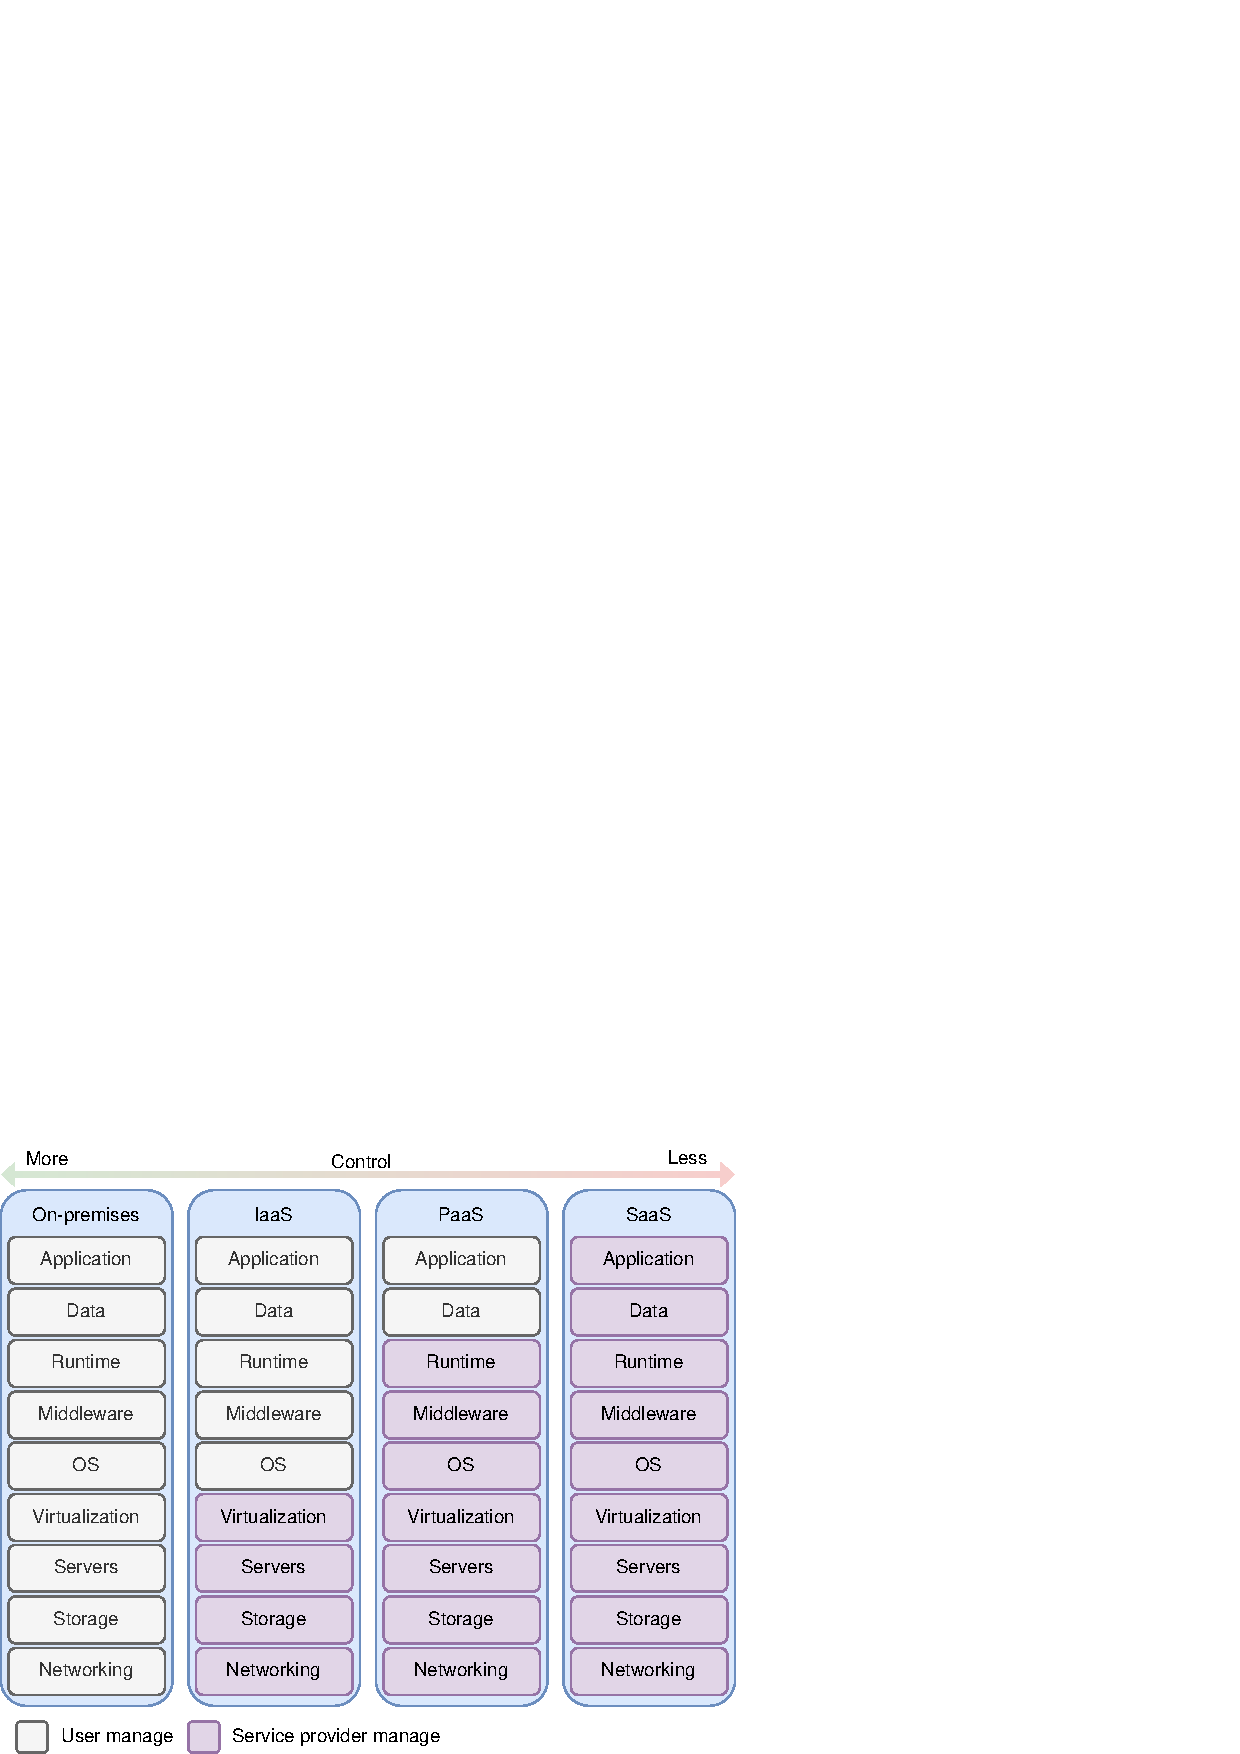
\includegraphics[scale=0.9]{images/Figure1.png}
	\end{center}
	\vspace{-0.6cm}
	\caption{Difference between cloud options and on-premises solution.}
	\label{fig:fig1}
\end{figure}

The user can choose a single solution, or combine more of them if such a thing is required depending on preferences and needs.

By the ownership, CC can be categorized into three categories:

\begin{itemize}
	\item \textbf{Public cloud} is type where CC is delivered over the internet, and shared across many many organizations and users. In this type of the CC, architecture is built and maintained by others. Users and organizations pay for what they use. Examples include: AWS EC2, Google App Engine, Microsoft Azure etc.
	\item \textbf{Private cloud} is type where CC is dedicated only to a single organization. In this type of the CC, architecture is built by organization who may offer their solution or services to the users or other organizations. These services are in domain what the organization does, and that organization is in charge of maintanance. Examples include VMWare, XEN, KVM etc.
	\item \textbf{Hybrid cloud} is such environment that uses both public and private clouds. Examples include: IBM, HP, VMWare vCloud etc.
\end{itemize}

Table~\ref{tab:table4} show comparison of public, private and hybrid cloud capabilities.

\begin{table}[h!]
	\begin{center}
		\begin{tabular}{l|l|l|l}
			\textbf{Capabilities} & \textbf{Public cloud} & \textbf{Private cloud} & \textbf{Hybrid cloud}\\
			\hline
			\textbf{Data control} & IT enterprise & Service Provider & Both \\
			\textbf{Cost} & Low & High & Moderate \\
			\textbf{Data security} & Low & High & Moderate \\
			\textbf{Service levels} & IT specific & Provider specific & Aggregate \\
			\textbf{Scalability} & Very high & Limited & Very high \\	
			\textbf{Reliability} & Moderate & Very high & Medium/High\\	
			\textbf{Performance} & Low/Medium & Good & Good \\
\end{tabular}
	\end{center}
	\vspace{-0.5cm}
	\caption{Comparison of public, private and hybrid cloud capabilities.}
	\label{tab:table4}
\end{table}

In the rest of the thesis, if not stated differently when CC term is used it denotes public cloud.

CC has been the dominating tool in the past decade in various applications~\cite{Satyanarayanan17}. It is changing, evolving, and offering new types of services. Resources such as container as a service (CaaS), database as a service (DBaaS)~\cite{Peter} are newly introduced. The CC model gives us a few benefits. Centralization relies on the economy of scale to lower the cost of administration of big DCs. Organizations using cloud services avoid huge investments. Like creating and maintaining their own DCs. They consume resources usually created by others~\cite{Satyanarayanan17} and pay for usage time -- a pay as you go model. 

But centralization give us few really hard problems to solve. As already stated in section~\ref{sec:problem_area} data is required to be moved to the cloud from data sources, which introduces a high latency in the system~\cite{HossainRH18}. 

There are few notable attempts to help data ingestion into the cloud. Remote Direct Memory Access (RDMA) protocol makes it possible to read data directly from the memory of one computer and write that data directly to the memory of another. This is done by using \textit{specialized hardware} interface cards and switches and software as well, and operations like read, write, send, receive etc. do not go through CPU. With this caracteristivs, RDMA have low latencies and overhead, and as such reach better throughputs~\cite{CohenTKCKRCDG09}. This new hardware may not be cheap, and not evey CC provider use them for every use-case. And this may not be enough, esspecially with ever growing amount of IoT devices and services.

Over the years there are more as a service options avalible, forming \textbf{everything as a service (XaaS)} model~\cite{DuanFZSNH15}. This model propose that any hardware or software resource can be ofered as a service to the users over the internet.

Table~\ref{tab:table2} shows common examples of SaaS, PaaS, and IaaS applications.

\begin{table}[h!]
	\begin{center}
		\begin{tabular}{l|l}
			\textbf{Platform type} & \textbf{Common Examples}\\
			\hline
			\textbf{IaaS} & AWS, Microsoft Azure, Google Compute Engine \\
			\textbf{PaaS} & AWS Elastic Beanstalk, Azure, App Engine \\
			\textbf{SaaS} & Gmail, Dropbox, Salesforce, GoToMeeting \\
		\end{tabular}
	\end{center}
	\vspace{-0.5cm}
	\caption{Common examples of SaaS, PaaS, and IaaS.}
	\label{tab:table2}
\end{table}

CC is giving a user an illusion that he is using single machine, while the backgroud implementaion is fairly complicated and consists of various elements that are composed of countles machines. CC is tipical example of horizontally scalable system presented in~\ref{sec:scalability}
%
%
\subsection{Membership protocol}\label{sec:memership_protocol}
%
A the start of this section we introduced DS, and we present two interesting assumptions by Tanenbaum et al.~\cite{SteenT16, 0019513}. If we take one more look at the~\ref{ds:asumption_2} assumption, we will see that user of the DS whether they are users or applications perceive DS as a single element. Inside this single elements nodes need to colaborate, so that they are albe to do various kinds of tasks.

Most basic of all these tasks, is that nodes needs to know which group they belog to, and who are their peers in the group they will colaborate with. This might sound as a trivial idea, but when we include 8 fallacies of the DS~\ref{ds:8_fallacies} into the equation, things start to be not so trivial, after all. In the setup where nodes are connected over the local network or internet, and they need to communicate things will go wrong for various reasons.

To resolve the problem that nodes need to know who are their group peers, a membership protocols come to help. These protocols needs to ensures that each process of one group updates his local list of \textbf{non-faulty} members of the group, and when a new process joins or leaves the group, local list for every process needs to be updated. This is the most basic idea behind membership protocols.

Processes in the group, or nodes in a group will ping each other in different ways, and using different strategies to figure out which nodes are dead and which are alive. There are few existing algorithms that does this job, and they are (usually) based on the way epidemics spread or how gossip is spreaded in population. Because of this feature these algorithms are usually called \textit{Gossip} style protocols.

Every membership protocol have some properties that will ensure efficiency and scalability:

\begin{enumerate}[start=1,label={(\bfseries \arabic*)}] \label{ds:features}
	\item \textbf{Completeness}, this property must ensure that every failure in the system is detected.
	\item \textbf{Accuracy}, in ideal world, there should be no mistakes when detecting failures. But In real life scenario, we need to reduce false positives as much as we can.
	\item \textbf{Failure detection speed}, all failures needs to be tected as fast as possible, in order to remove the node from the group and reschedule the tasks from dead node to alive ones.
	\item \textbf{Scale}, with this property we must ensure that the network load that is generated should be distributed equally between all processes in the group.
\end{enumerate}

Easiest idea to implement this protocol would be \textbf{heartbeating} technique where process $P_i$ will send heartbeat message to all his peers in the group or \textbf{multicast}. After some time if process $P_j$ did not receive heartbeat message from $P_i$, it will mark him as faild. This idea is easy to understand, and implement but downsides are that his process is not really \textbf{scalable}, esspecially for large groups, and this will introduce huge network traffic.

To resolve this problem, Das et al.~\cite{DasGM02} introduced \textbf{S}calable \textbf{W}eakly-consistent \textbf{I}nfection-style Process Group \textbf{M}embership protocol, or \textbf{SWIM} for short. This protocol divides the membership problem into two parts:

\begin{enumerate}[start=1,label={(\bfseries \arabic*)}]
	\item \textbf{Failure detection}, this component works so that one node will select random node in the group, and it will send him $ping$ message, expecting $ack$ message in return --- \textbf{direct ping}. If such message is not received, he will pick $n$ nodes to probe through a $ping-req$ message --- \textbf{indirect ping}. If this fail, node will be marked as $suspected$, and it will be marked as $dead$ after some timeout. If node get alive, he will ping some other node and he will get back into the group. Figure~\ref{fig:fig15} show message passing in \textbf{direct} $(left)$, and \textbf{indirect} $(right)$ ping in SWIM protocol.
	\item \textbf{Information dissemination}, with previous strategy, we can disseminate information by piggybacking the data on multiple messages ($ping$, $ping-req$ and $ack$), and avoid using the multicast solution.
\end{enumerate}

\begin{figure}[H]
	\begin{center}
		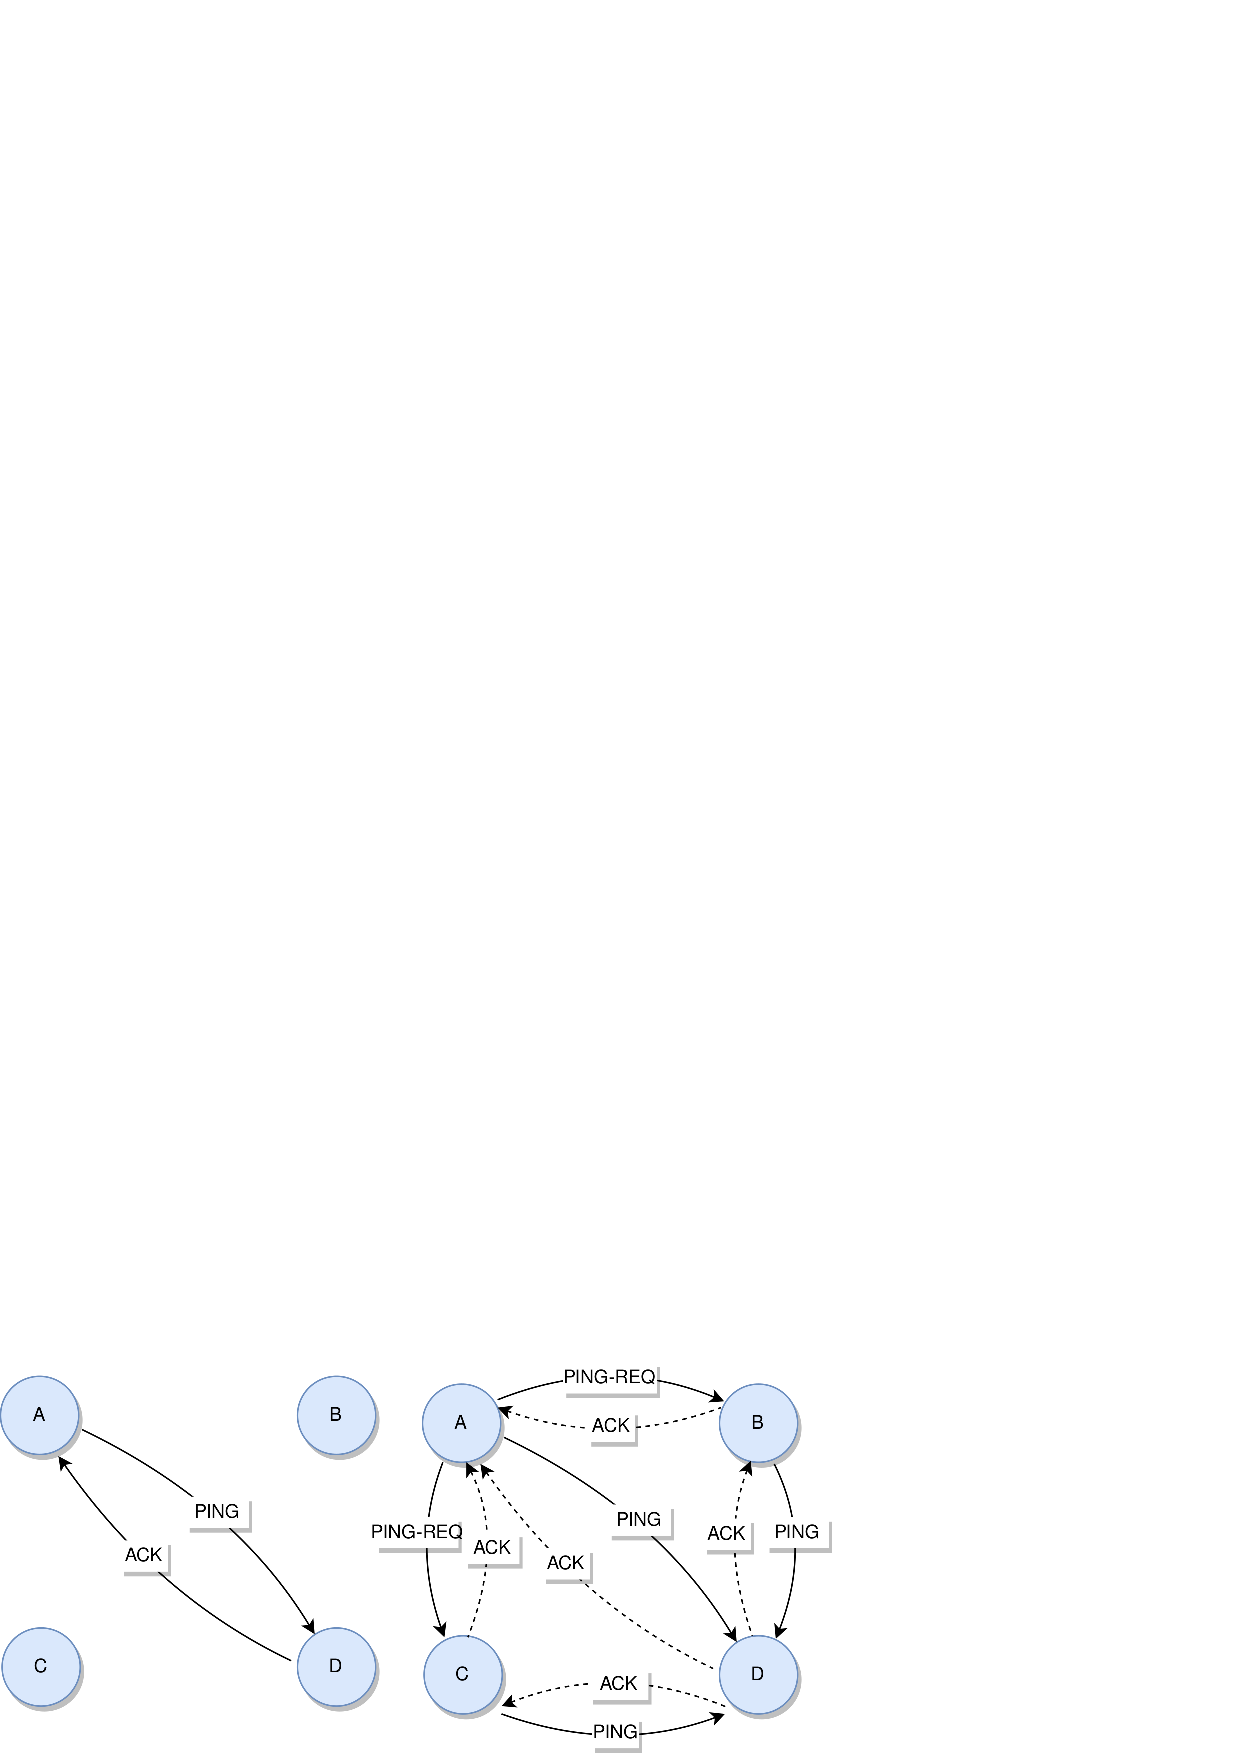
\includegraphics[scale=0.7]{images/Figure15.png}
	\end{center}
	\vspace{-0.6cm}
	\caption{Direct and indirect ping in SWIM protocol.}
	\label{fig:fig15}
\end{figure}

Over the years, reserchers foud ways to improve the protocol for example Dadgar et al. present Lifeguard protocol~\cite{DadgarPC18} for more
acccurate failure detection, and there are other implementations to fine tune the SWIM, but base idea is still there. Today SWIM or SWIM-like protocols are standard membership procol whenever we are doing some node clustering.
%
%
\subsection{Mobile computing}\label{sec:mobile_computing}
%
Mobile cloud computing (MCC), was the first idea that introduced task offloading~\cite{FernandoLR13, LinLJL19}. Heavy computation remains in the cloud. Mobile devices run small client software and interact with the cloud, over the internet using his resources. 

The main problem with MCC is that the cloud is usually far away from end devices. That leads to high latency and bad quality of experience (QoE)~\cite{LinLJL19}. Especially for latency-sensitive applications. Even though MCC is not that much different from the standard cloud model. We had moved a small number of tasks from the cloud. Thus opening the door for future models.

To overcome cloud latency and MCC problems, research led to new computing areas like edge computing (EC). EC is a model in which computing and storage utilities are in proximity to data sources~\cite{Satyanarayanan17}. The cloud is enhanced with new ideas for future generation applications~\cite{NingLSY20}. 

Over the years, designs like fog~\cite{BonomiMNZ14}, cloudlets~\cite{MonsalveCC18}, and mobile edge computing (MEC)~\cite{WangZZWYW17} emerged. In this thesis, we refer to all these models as edge nodes. They all use the concept of data and computation offloading from the cloud closer to the ground~\cite{KhuneP19}, while heavy computation remains in the cloud because of resource availability~\cite{NingLSY20}. 

EC models introduce small-scale servers that operate between data sources and the cloud. Typically, they have much less capabilities compared to the cloud counterparts~\cite{ChenHLLW15}. These servers can be spread in base stations~\cite{WangZZWYW17}, coffee shops, or over geographic regions to avoid latency as well as huge bandwidth~\cite{MonsalveCC18}. They can serve as firewalls~\cite{SatyanarayananK19} and pre-processing tier, while users get a unique ability to dynamically and selectively control the information sent to the cloud.
%
%
\section{Distributed computing}\label{sec:distributed_computing}
%
DC can be defined as the use of a DS to solve one large problem by breaking it down into several smaller parts, where each part is computed in the individual node of the DS and coordinatio is done by passing messages to one another~\cite{0019513}. Computer programs that use this strategy and runs on DS are called \textbf{distributed programs} \cite{Vera16, andrews2000foundations}. 

Similar to CC in Section~\ref{sec:cloud_computing}, to a normal user, DC systems appear as a single system similar to one he use every day on his personal computer. DC share same fallacies to DS presented in~\ref{sec:distributed_systems}.
%
%
\subsection{Big Data}\label{sec:big_data}
%
Tearm big data means that the data is unable to be handled, processed or loaded into a single machine~\cite{FisherDCD12}. That menas that traditional data mining methods or data analytics tools developed for a centralized processing  may not be able to be applied directly to big data~\cite{Tsai2015}. 

New tools and methos that are developed are relying on DS and one specific feature \textbf{data locality}. Data locality can be described as a process of moving the computation closer to the data, instead of moving large data to computation~\cite{GuoFZ12}. This simple idea, minimizes network congestion and increases the overall throughput of the system.

In~\ref{sec:problem_area} we already give two examples how huge generated data could be, and when we incude other IoT sensors and devices these numbers will just keep getting bigger~\cite{SarigiannidisLR20}.

On contrary to relational databases that mostly deal with structured data, big data is dealing with various kinds of data~\cite{FisherDCD12, Tsai2015, GuoFZ12}:

\begin{itemize}
	\item \textbf{Structured} data is kind of data that have some fixed structure and format. Tipical example of this is data stored inside table of some database. organizations susully have no huge problem extracting some kind of value out of the data.
	\item \textbf{Unstructured} data is kind of data where wo do not have any kind of structure at all. These data sources are heterogeneous and may containing a combination of simple text files, images, videos etc. This type of data is usully in raw format, and organizations have hard time to derive value out.
	\item \textbf{Semi-structured} data is kind of data that can contain both previously mentioned types of data. Example of this type of data is XML files.
\end{itemize}

Along it's share size, big data have other instantly recognizable features called \textbf{V's} of big data~\cite{PatgiriA16}. Name is derived from starting letters from the other features that are describing big data. Image~\ref{fig:fig3} show 6 V's comonly used to represent the big data.

\begin{figure}[H]
	\begin{center}
		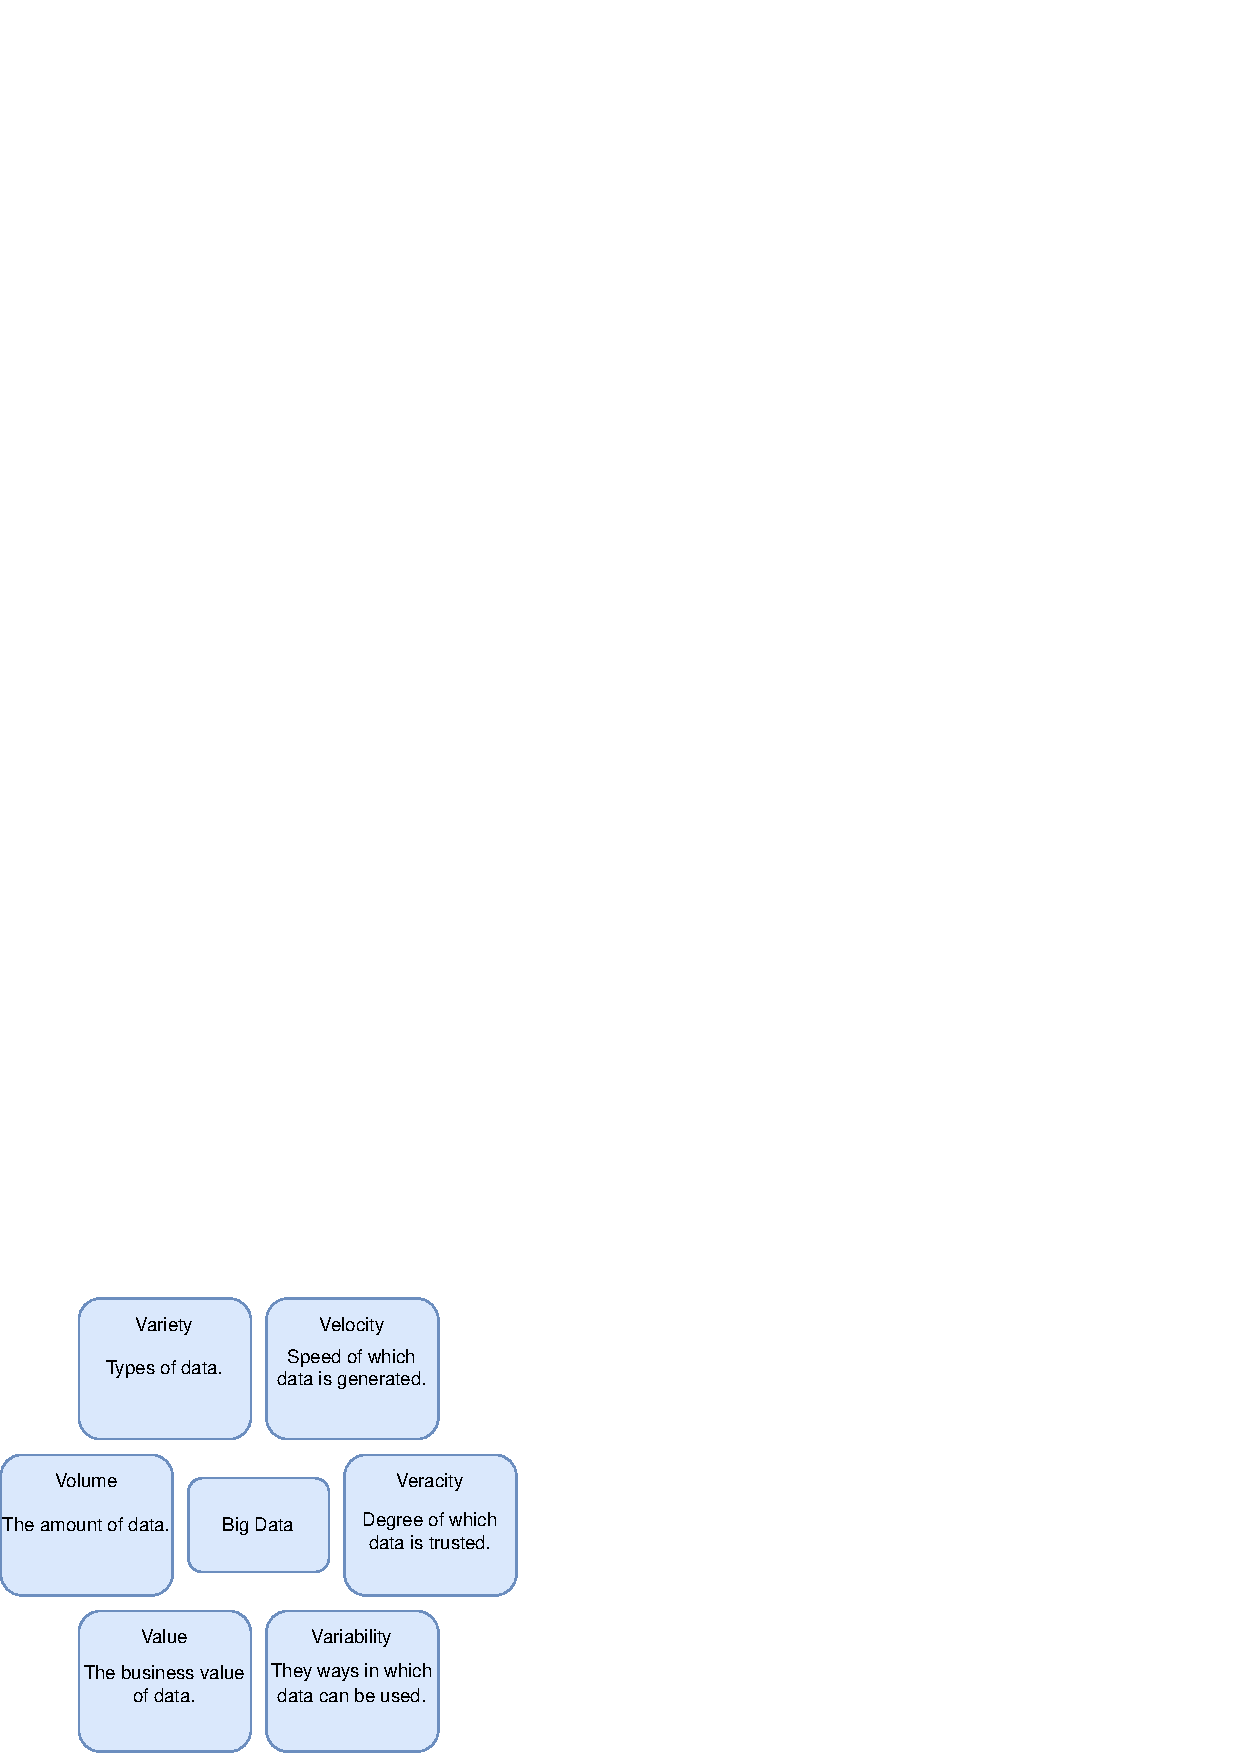
\includegraphics[scale=0.7]{images/Figure3.png}
	\end{center}
	\vspace{-0.6cm}
	\caption{V's of Big Data.}
	\label{fig:fig3}
\end{figure}

Processing in big data systems can be represented as~\cite{phdthesis, KiranMMDB15}:

\begin{itemize}
	\item \textbf{Batch processing} represents data prcessing technique that is done on huge quantity of the stored data. This type of prcessing is usually slow and requure time.
	\item \textbf{Stream processing} represents data processing technique that is done as data get into the system. This type of processing is usually done on smaller quantity of the data \textbf{at the time}, and it is faster.
	\item \textbf{Lambda architectures} represents processing technique where stream processing and handling of massive data volumes in batch are combined in a uniform manner, reducing costs in the process~\cite{KiranMMDB15}.
\end{itemize}

Big data systems, are not processing and value extracting systems. Big data systems can be separated in few categories: $(1)$ data storage, $(2)$, data ingestion $(3)$, data processing and analytics. All these system aids to properly analyze ever growing requirements~\cite{RaoMBG19},

Dispite promise that big data offers to derive value out of the collected data, this task is not easy to do and requre properly set up system filtering and removeing data that contains no value. To aid this idea, data could be filtered and little bit preprocessed on close to the source~\cite{inproceedingsSimic1}, and as such sent to data lakses~\cite{MarynowskiSP15}.
%
%
\subsection{Microservices}\label{sec:microservices}
%
There is no single comperhensive deffinition of what a microservice is. Differnet people and organizations use different definition do describe them. A working definition is offered in~\cite{DragoniGLMMMS16} as~\say{s microservice is a cohesive, independent process interacting via messages}. Despite lack of comperhensive definition all agree on few features that come with microservices: 

\begin{enumerate}[start=1,label={(\bfseries \arabic*)}]
	\item they are small computer programs that are independently deployable and developed.
	\item they coud be developed using different languages, principles and using differend databses.
	\item they communicate over the network to achieve some goal.
	\item they are organized around business capabilities~\cite{PautassoZALJ17}.
	\item they are implemented and mainteined by a small team.
\end{enumerate}

Industry is migrating much of their applications to the cloud, because CC offers to scale their computing resources as per their usage~\cite{LiZJLZLGGS19}. Microservices are small loosely coupled services that follos UNIX philosophy~\say{do one thing, and do it well}~\cite{krause2015microservices}, and they communicate over well defined API~\cite{DragoniGLMMMS16}.

This architecure patter is well aligned to the CC paradigm~\cite{LiZJLZLGGS19}, contrary to previous models like monolith whose modules cannot be executed independently~\cite{DragoniGLMMMS16, abs-1905-07997}, and are not well aligned with the CC paradigm~\cite{abs-1905-07997}. Table~\ref{tab:table3} summrize differences between monolith and microservie architecture.

\begin{table}[h!]
	\begin{center}
		\begin{tabular}{l|l|l}
			\textbf{Feature} & \textbf{Monolith} & \textbf{Microservices}\\
			\hline
			\textbf{Structure} & Single unit & Independent services \\
			\textbf{Management} & Usually easier & Add DS complexity\\
			\textbf{Scale/Update} & Entire app & Per service \\
			\textbf{Error} & Usually crush entire app & App continue to work \\
		\end{tabular}
	\end{center}
	\vspace{-0.5cm}
	\caption{Differences between horizontall and verticall scaling.}
	\label{tab:table3}
\end{table}

Since their inception, microservices architecture is gone through some adaptations. And modern day microservices are extended with two new models each with it's unique abilities and problems:

\begin{itemize}
	\item \textbf{Cloud-native applications}, are specially designed applications for CC. They are distributed, elastic and horizontal scalable system by their nature, and composed of (micro)services which isolates state in a minimum of stateful components~\cite{KratzkeQ17}. These type of applications are self-contained, could be deployed independently, and they are composed of loosely coupled microservices that are packaged in lightweight containers. They have Improved resource utilization, and they are centered around APIs.
	\item \textbf{Serversles applications} is computing model, where the developers need to worry only about the logic for processing client requests~\cite{AdzicC17}. Logic is represented as event handler that only runs when client request is received, and billing is done only when these functions are executing~\cite{AdzicC17}. \textbf{Cold start} is one of features of the severless computing, and we can define it as user requests need to wait, until new container instance is up and running before can do any processing at all. Most providers have 1–3 second cold starts, and this is important for certain types of applications where latency is concern. Cold start is only happening when there are no \textit{warm} containers available for the request, meaning there is no single instance to server request. Other features include: $(1)$ simplified services development, $(2)$ faster time to market, $(3)$ and lower costs.
	\item \textbf{Service Mesh} is designed to standardize the runtime operations of applications~\cite{LiLGZH19}. As part of the microservices ecosystem,
	this dedicated communication layer can provide a number of benefits, such as: $(1)$ observability, $(2)$ providing secure connections, or $(3)$ automating retries and backoff for failed requests. With these features, developers only focus on implementation of buisniss logic, while operators gain out-of-the-box traffic policies, observability, and insights from the services. Advocates of microservice movemant, nowdays recommend using service mesh architecture when running microservices in production environments.
\end{itemize}

Microservices communicate over a network to fulfil some goal using message passing technique and technology-agnostic protocols such as HTTP. They can be implemented as:

\begin{itemize}
	\item Representational state transfer (REST) services~\cite{AdamczykSJH11}, is an architectural style with set of constraints that users can create web srevices and interoperability between computer systems on the internet. It is based on HTTP routs to define resources, and used HTTP verbs to represent operations over these resources. It relys on textual based communications, and payload could be represented using $JSON$, $XML$, $HTML$ etc.
	\item Remote procedure calls (RPC) represent architectural way to design services that are able to call subroutines that are located in different places, usually on other machine. Client is calling these operations like they are located localy in his address space.
	\item Event-driven services, are services where communicatoin between services is done using events. Events are sent on some channel and other read messages that are received on other channel. These channels could be implemented either like message queues or message topics. Services connect to message queu or subscribe to the specific topic, and when messige arive, they can act acording to message type.
\end{itemize}
 
 They are well aligned with text based protocols like HTTP/1 using $JSON$ for example, or binary protocols such as HTTP/2 using $protobuf$ and $gRPC$ for example, and even new faster version like HTTP/3 over new $QUIC$ protocol, designed by Google. HTTP 3 is the latest version of the conventional and trusted HTTP protocol. It is very similar to HTTP 2, but it also offers a few important new features. Table~\ref{tab:table9} show important difference between versions of HTTP protocol.
 
 \begin{table}[h!]
 	\begin{center}
 		\begin{tabular}{l|l|l|l}
 			\textbf{Feature} & \textbf{HTTP1} & \textbf{HTTP2} & \textbf{HTTP3}\\
 			\hline
 			\textbf{Transport} & text & binary & binary\\
 			\textbf{Parallelism} & No & Yes & Yes\\
 			\textbf{Protocol} & TCP & TCP & QUIC \\
 			\textbf{Space} & OS level & OS level & User level\\
 			\textbf{Server push} & No & Yes & Yes\\
 			\textbf{Compression} & Data & Data/Headers & Data/Headers\\
 		\end{tabular}
 	\end{center}
 	\vspace{-0.5cm}
 	\caption{Idempotent and non-idempotent operations.}
 	\label{tab:table9}
 \end{table}
 
 To enshure vider range of devices that are able to comunicate with the rest of the systems, developrs usually have a gateway into the system that is REST service, and other services could be implemented in different way.

It is important to point out, that all flavors of microservices applications rely on continuous delivery and deployment~\cite{7436659}. This is enabled by lightweight containers, instead of virtual machines~\cite{FelterFRR15}, and orchestration tools such Kubernetes~\cite{BurnsGOBW16}. These concepts wll be described in more detail in Section~\ref{sec:virtualization_techniques}.

Microservices architecture are good starting point especially for build as a service applications, and applications that should serve huge amount of requests and users. Esspecially with benefits of CC to pay for usage, and ability to scale parts of the system independently.  Although they are not necessarily easy to implement properly. There are more and more critique to the architecture model~\cite{SoldaniTH18}. Microservices are relying and use parts of the DS, and as such they inherit almost all problems DS has. 

One particilar thing that users need to be aware of is \textbf{idempotency}. In microservices applications, developers are dealing with inconsistencies in distributed state, and their operations should be implemented as idempotent. An operation is idempotent if it will produce the same results when executed over and over again. It is a strategy that means that operations with sade effects like creation or deletion can be called any number of times, while guaranteeing that side effects only occur once. Idempotency is term that come from mathematics, and can be represented by simple idempotency law for operation $*$ like~\cite{gratzer2002general}:

\begin{equation}\label{form:idempotency_law}
	\forall x, x * x = x
\end{equation}
\myequations{Idempotency law formula}

Not all Create, Read, Update, Delete (CRUD) operations are idempotent by default. But developers need to make effort to make all of them idempotent, to prevent bad outcomes and incosistant state. 

Table~\ref{tab:table8} show list of idempotent and non-idepotent for standard CRUD operations:

\begin{table}[h!]
	\begin{center}
		\begin{tabular}{l|c|c}
			\textbf{Operation} & \textbf{Idempotent} & \textbf{Non-idempotent}\\
			\hline
			\textbf{Create} &  & x \\
			\textbf{Read} & x & \\
			\textbf{Update} & x & \\
			\textbf{Delete} & x & \\
		\end{tabular}
	\end{center}
	\vspace{-0.5cm}
	\caption{Idempotent and non-idempotent operations.}
	\label{tab:table8}
\end{table}

Crate operation is not idempotent by default, but to make it idempotent there are multiple strategies how to do so. Most comon way is to create \textbf{idempotency key} that will be sent in the request, and based on that request server can decide is this operations already invoked or not. If server is already \say{seen} specified idempotency key, than operation is already done and we can return just responce that operation is done but no operation will be done over the state of the service or application. If server see idempotency key for the first time, that is the signal that this request is new one, and it should be done.

Idempotency key could be stored in any kind of the storage, it is not uncommon that these keys are stored in cache storage with some time to live (TTL) policy that will automatically remove the key after specified time.

Other option that is comonly used is hasing user specified actions. This is usefull to know what part of action set is already done and what is not. This strategy is used in scenarios where we must preserve order of actions.

Best chance to success when implementing microservices architecture, is to simply follow existing patters and use existing solutions with proven quality.
%
%
\section{Distribution Models}\label{sec:distribution_models}
%
The role of distribution models is to determine the responsibility for the request, or to answer the fundamental question \say{who is in charge} for specific request. There are two ways to answer this question: $(1)$ all nodes in the system, or $(1)$ single node in the system.
%
%
\subsection{Peer-to-peer}\label{sec:p2p_networks}
%
Peer-to-peer (P2P) communication is a networking architecture model that partitions tasks or workloads between peers~\cite{Schollmeier01}. All peers are created equally in the system, and there is no such thing as a node that is more important then others. Every Peer have a portion system resources, such as processing power, disk storage or network bandwidth, directly available to other network participants, without the need for central coordination by servers or stable hosts~\cite{Schollmeier01}. P2P nodes are connected and share resources without going through a separate server computer that is responsabile for routing. Figure~\ref{fig:fig2} show difference in network topology between P2P networks $(left)$ and client-server architecture $(right)$.

\begin{figure}[H]
	\begin{center}
		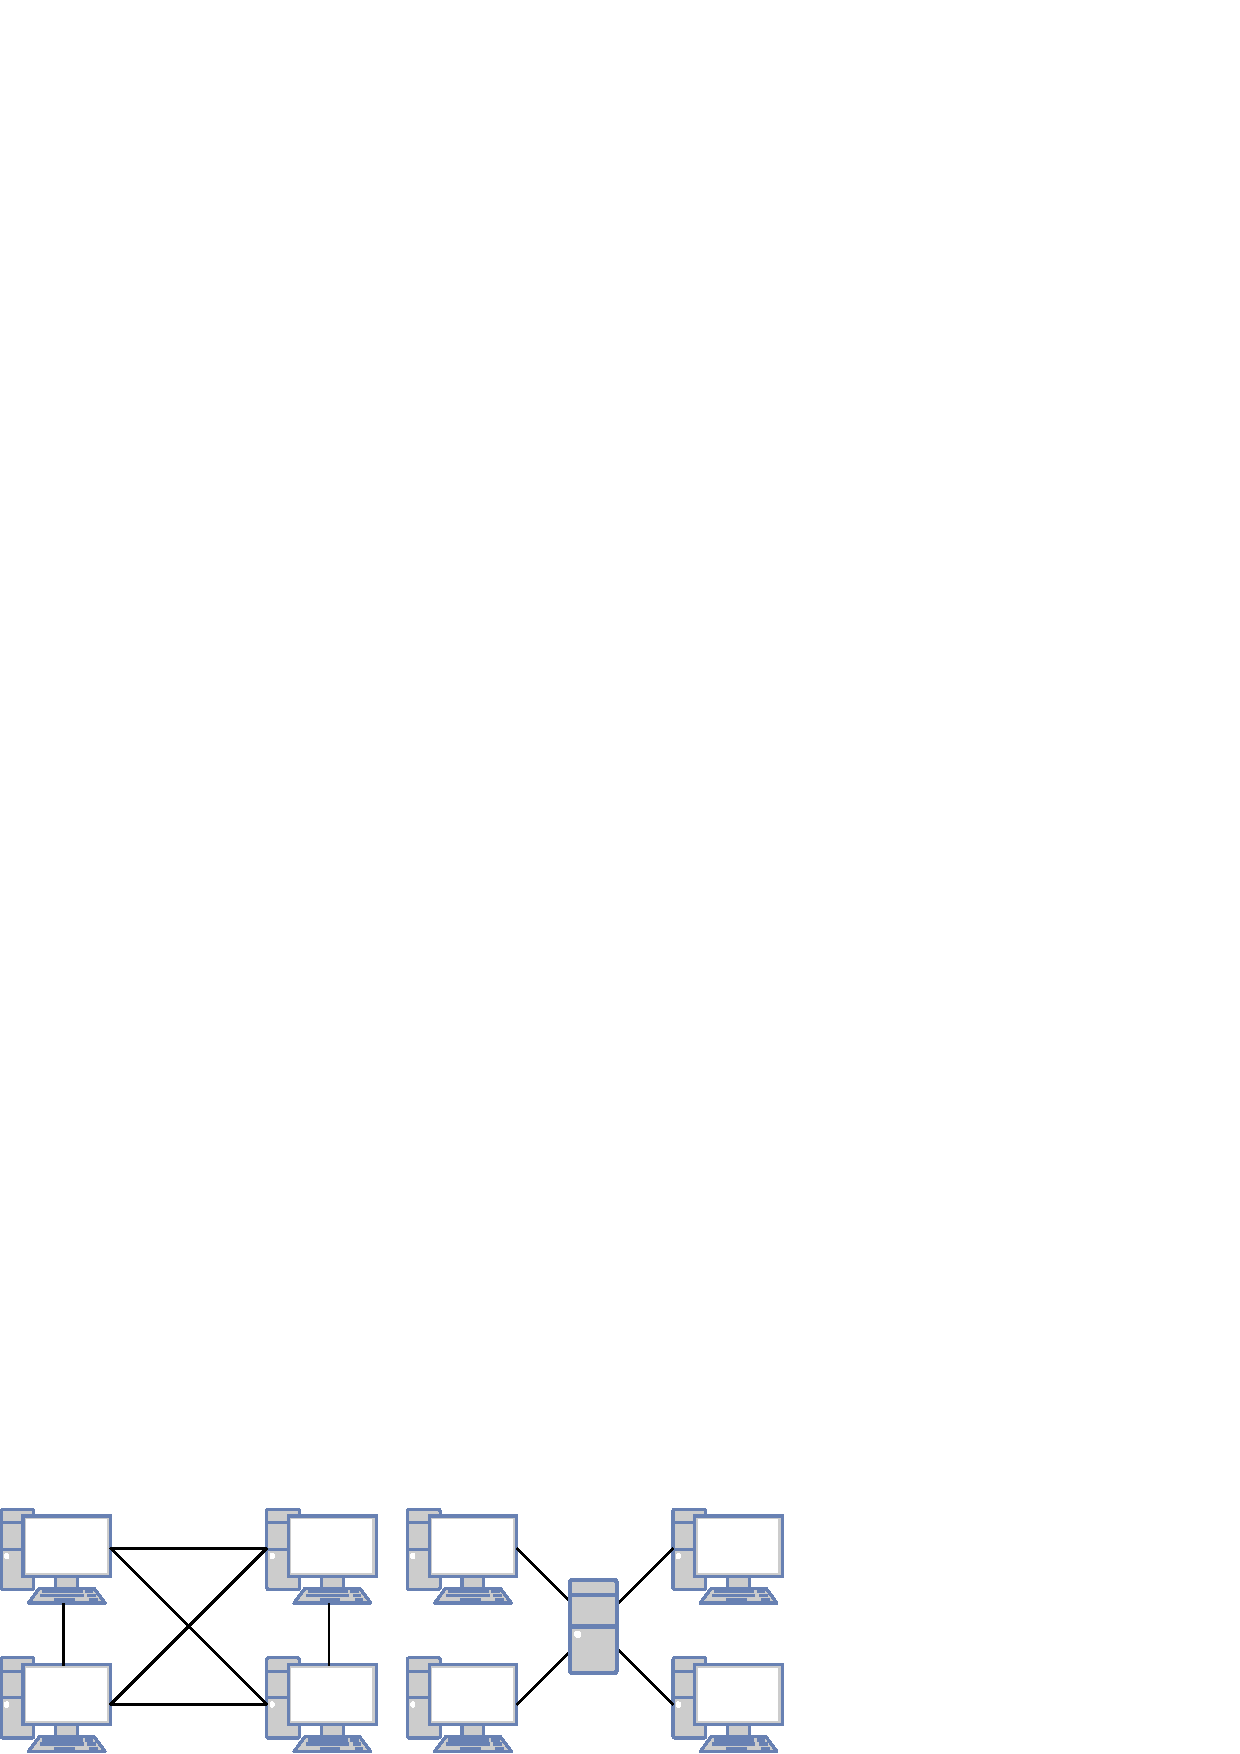
\includegraphics[scale=0.7]{images/Figure2.png}
	\end{center}
	\vspace{-0.6cm}
	\caption{P2P network and client-server network.}
	\label{fig:fig2}
\end{figure}

Peers are creating a sense of virtual community. This community of peers can resolve a greater tasks, beyond those that individual peers can do. Yet, these tasks are beneficial to all the peers in the system~\cite{BandaraJ13}. When request come to such network, node that accepted request is usually called \textbf{coordinator}, because he then is trying to found the right peer to send request to.

Based on how the nodes are linked to each other within the overlay network, and how resources are indexed and located, we can classify networks as~\cite{KamelSE07}:

\begin{itemize}
	\item \textbf{Unstructured} do not have a particular structure by design, but they are formed by nodes that randomly form connections~\cite{FilaliBHB11}. Their strenght and weaknes at the same time is ther lack of structure. These networks and robust when peers join and leave network. But when doing query, they must found more possible peers that have same peace of data. Tipical example of this group is a Gossip-based protocols like~\cite{DasGM02}.
	\item \textbf{Structured} peers are organized into a specific topology, and the protocol ensures that any node can efficiently search the network for a resource. The famos type of structured P2P network is a Distributed Hash Table (DHT). These networks maintain lists of neighbors to do more efficent lookup, and as such they are not so robust when nodes join or leave the network. DHT commonly used in resource loopkup systems~\cite{StoicaMKKB01}, and as efficent resource lookip management and scheduling of applications, or as an integral part of distributed storage systems and NoSQL\cite{Leavitt10} databases.
	\item \textbf{Hybrid} combine previous two models in various ways.
\end{itemize}

P2P networks are great tool in many arsenals, but because their unique ability to act as a server and as a client at the same time we must be aware and pay more attention to security because they are more vulnerable to exploits~\cite{0024003}.
%
%
\subsection{Master-slave}\label{sec:master_slave}
%
In the master-slave architecture, there is one node that is in charge -- \textbf{master}. This node accespt requests, and we usually do not communicate to rest of nodes or \textbf{slaves}. Master node is usually better and more expensive or even specialized hardware such as RAID drives to lower the crush probability. The cluster can also be configured with a \textbf{standby} master, and this node is continually updated from the master node.

But no metter how specialized hardware master runs on, it is prone to fail for varios reasons, so he is a \textbf{single point of failure}. If crush happend, than standby master could continue to server as a master, or new \textbf{leader election} protocol~\cite{KorachKM90} is initiated to pick new master node. 

Master node is responsible for processing any updates to that data. If the master fails, than  the slaves can still handle read requests. Failure of the standby master node, to take over from the master node is a real problem if we want to achieve high-availability system.

Figure~\ref{fig:fig16} show difference between mater-slave $(left)$ and peer-to-peer $(right)$ request handling.

\begin{figure}[H]
	\begin{center}
		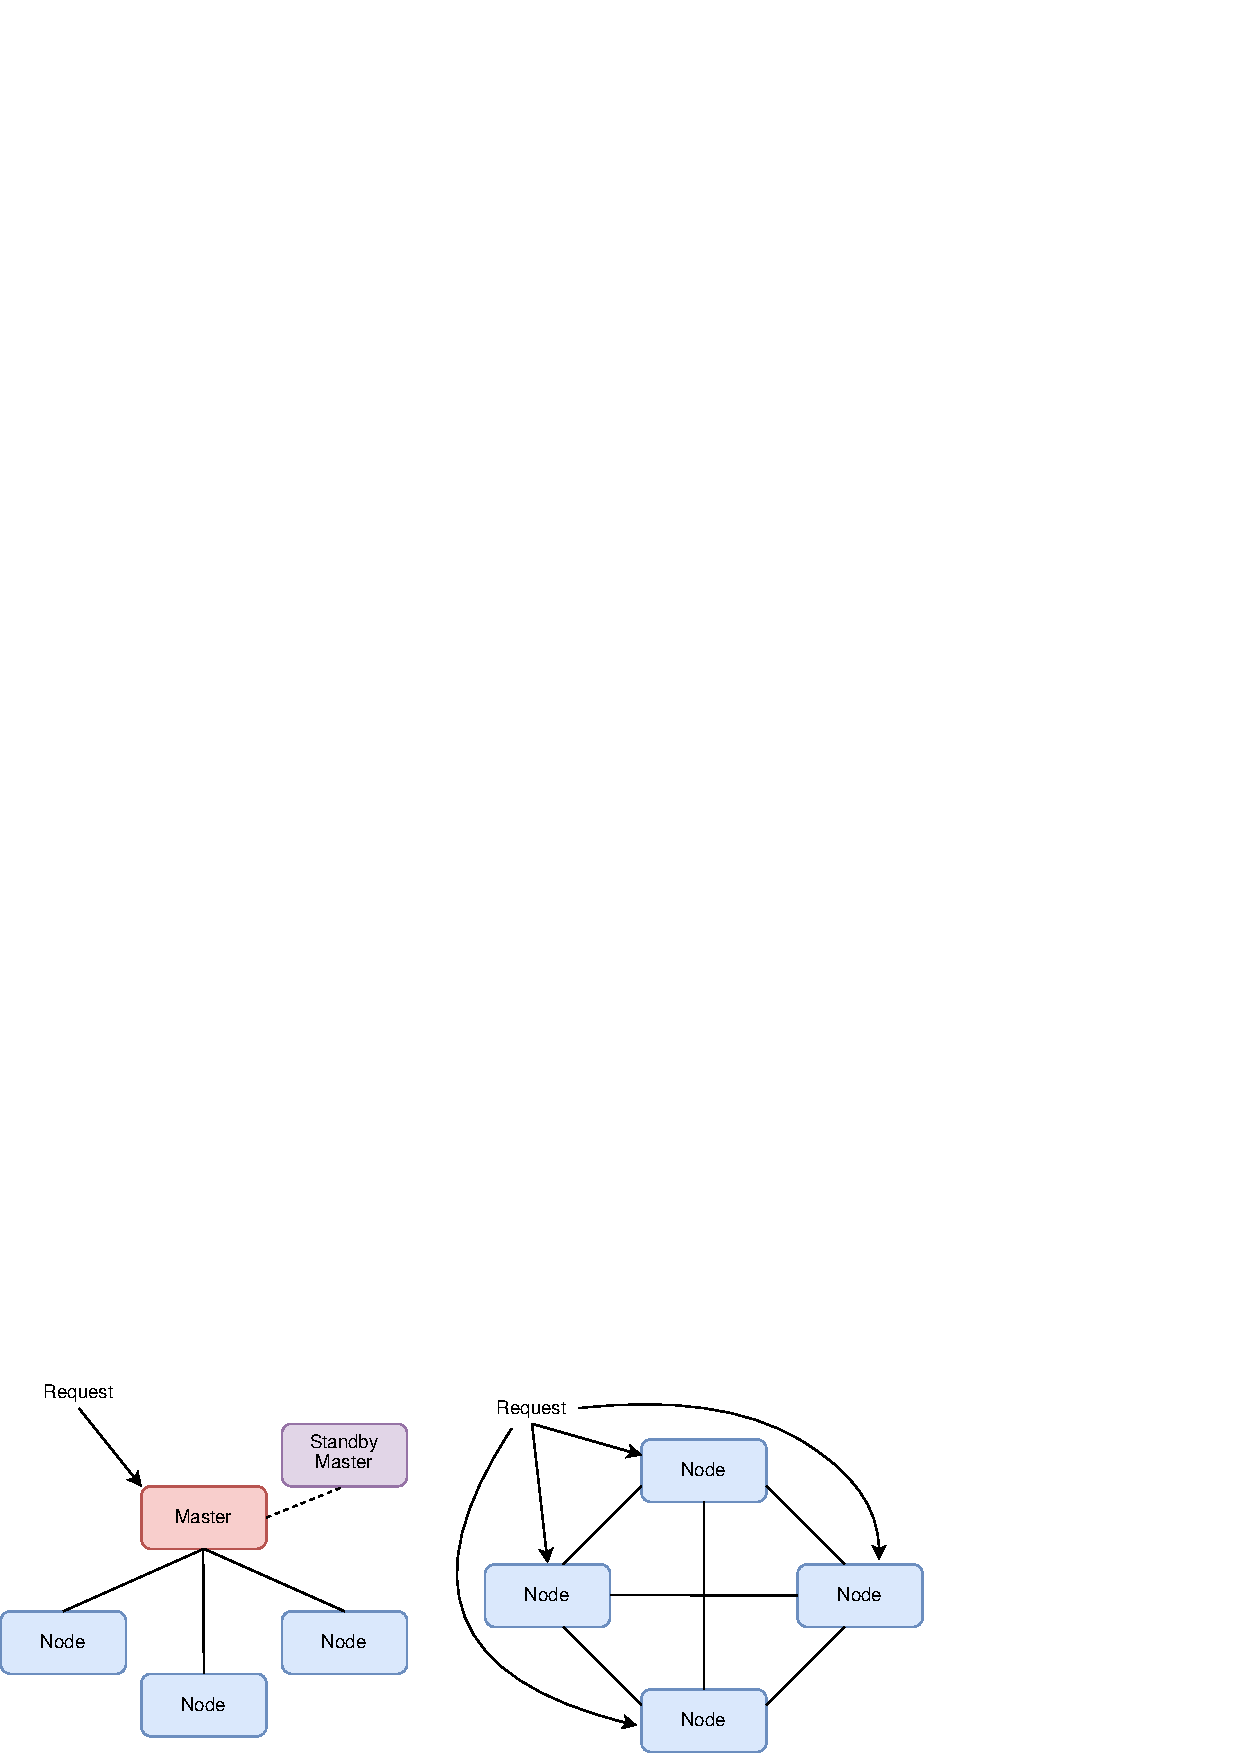
\includegraphics[scale=0.7]{images/Figure16.png}
	\end{center}
	\vspace{-0.6cm}
	\caption{Handling requests master-slave and peer-to-peer}
	\label{fig:fig16}
\end{figure}

Using the right distribution model usually depends on the business requirements. High availability requires a P2P network because no single point of failure. If we could manage data using batch jobs that run in off hours, then the simpler master-slave model might be the solution.
%
%
\section{Similar computing models}\label{sec:similar_models}
%
In this section we are going to shortly describe models that are similar to the DS, and as such they may be the source of confusion.
%
%
\subsection{Parallel computing}\label{sec:parallel_computing}
%
DC and parallel computing seems like models that are the same, and that may share some features like simultaneously executing a set of computations in parallel. Broadly speaking, this is not far from the truth~\cite{Vera16}. 

Distinguished between the two can be presented as follows: in parallel computing all processor units have acces to the shared memory and have some way of the faster inter-process communication, while in DS and DC all processors have their own memory on their own machine and communicate over network to other nodes which is significantly slower. 

These models are similar, but they are not indentical, and the kind of problems they are designed to work on are different. Figure~\ref{fig:fig4} visually summarize the architectural  differences between DC $(up)$ and parallel computing $(down)$.

\begin{figure}[H]
	\begin{center}
		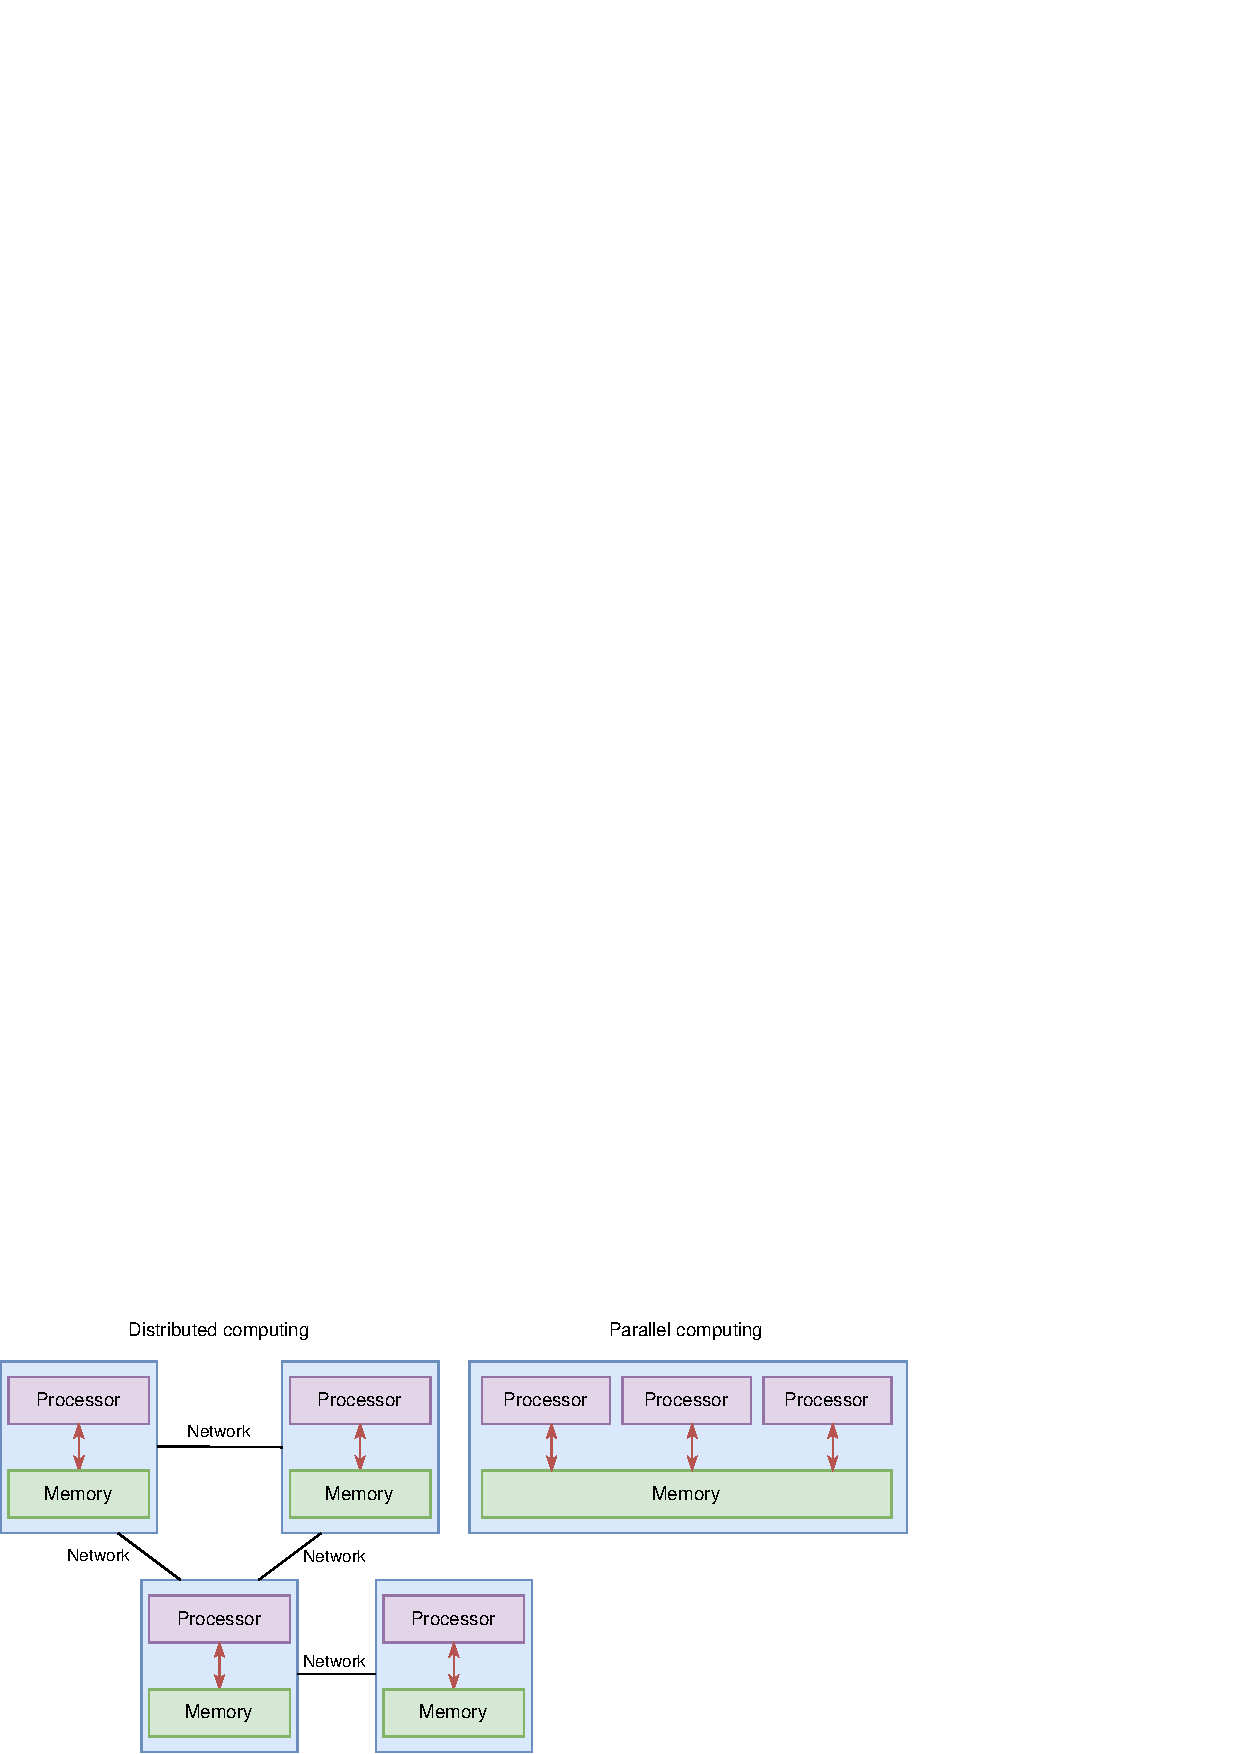
\includegraphics[scale=0.8]{images/Figure4.png}
	\end{center}
	\vspace{-0.6cm}
	\caption{Architectural difference between DC and parallel computing.}
	\label{fig:fig4}
\end{figure}

Parallel computing is often used strategy with problems, that due to their nature or constraints must be done on multi-core machines simultaneously~\cite{0072397}. It is ofthen, that huge problems are divided into smaller ones, which can then be solved at the same time. 

There are number of tasks that requre parallel computing like simulations, computer graphics rendering or different scenarios in scientific computing.
%
%
\subsection{Decentralized systems}\label{sec:decentralized_systems}
%
Decentralized systems are similar to DS, in technical sense they are still DS. But if we take closer look, these systems \textbf{should not} be owned by the single entity. CC for example is perfect example of DS, but it is not decentralized by it's nature. It is centralized systems by the owner like AWS, Google, Microsoft or some other private compay because all computation needs to be moved to big DCs~\cite{HossainRH18}.

By today standards, when we are talking about decentralyzed systems, we usually think of blockchain or blockchain-like technology~\cite{LeibleSSG19}. Since here we have distributed nodes, that are scattered and there is no single entity that own all these nodes. But even if this technology is run in the cloud, it is loosing the decentralized feature. This is the caveat we needs to be aware of. These systems are facing different issues, because any participent in the system might be malicious and they need to handle this case. 

Nontheless, CC can and should be decentralized in a sense that some computation can happend outside of cloud big DCs, closer to the sources of data. These computation could be owned by someone else, and big cloud companies could give their own solution to this as well to relax centralization and problems that CC will have esspecially with ever growing IoT and mobile devices.
%
%
\section{Virtualization techniques}\label{sec:virtualization_techniques}
%
Virtualization as a technique started long ago in time-sharing systems, to provide isolation between multiple users shareing a single system liek a mainframe computer~\cite{CrosbyB06}. 

In~\cite{Sharma} Sharma et al. describe virtualization as technologies which provide a layer of abstraction of the physical computing resources between computer hardware systems and the software systems running on them.

Modeern virtualization diferentiate few different tools. Some of them are used as an integral part of the infrastructure for some flavors like IaaS, while others are used in different CC flavors as well as microservices packageing and distribution format, or are new and still are looking for their place. These options are:

\begin{itemize}
	\item \textbf{Virtual machines (VM)} are the oldest tehnology of the three. In~\cite{Sharma} Sharma et al. describe them as a self-contained operating environment consisting of guest operating system and associated applications, but independent of host operating system. VMs enable us to pack isolation and better utilization of hardware in big DCs. They are vidly used in IaaS environment~\cite{AbsalomBJ13, YangHCLW13} as a base where users can install theirown operating system (OS) and required software tools and applications.
	\item \textbf{Containers} provide almost same functionality to VMs, but there are several subtle differences that make them a goto tool in modern develpment. Instead of the guest OS running on top of host OS, containers use tools that are in Linux kernles like \textit{cgroups} that limits process resource usage so that single process can not starve other processes and use all the resources for himself, and \textit{namespaces} to provide isolation and partitions kernel resources so that single process see node resources like he only exists there. Containers reduce time and footprint from development to testing to production, and they utilize even more hardware resources compared to VMs and show better performance compared to the VMs~\cite{Seo2014PerformanceCA, FelterFRR15}. Containers provide easier way to pack servies and deploy and they are esspecially used in microservices architecture and service orchestration tools like Kubernetes~\cite{BurnsGOBW16}. Google stated few times in their on-line talks that hey have used container technology for all their services, even they run VMs inside containers for their cloud platform. Even though they exist for a while, containers get popularized when companies like Docker and CoreOS developed user-friendly APIs.
	\item \textbf{Unikernels} are the newest addition to the virtualization space. In~\cite{pavlicek2016unikernels} Pavlicek define unikernels as small, fast, secure virtual machines that lack operating systems. Unikernels are comprised of source code, along with only the required system calls and drivers. Because of their specific design, they have single process and they contains and executes what it absolutely needs to nothing more and nothing less~\cite{GoethalsSAVT18}. They are advertised that new technology that will safe resources and that they are \textit{green}~\cite{208735} meaning they save both power and money. When put to the test and compared to containers they give interesting results~\cite{GoethalsSAVT18, PlauthFP17}. Unikernels are still new technology and they are not widly adopted yet. But they give promessing features for the future, esspecially \textbf{if} properly ported to ARM architectures, and various development languages. Unikernes will probably be used as a user applications and functions virtualization tool, because their specific architecture, esspecailly for serverless applications presened in~\ref{sec:microservices}.
\end{itemize}

Figure~\ref{fig:fig5} represent architectural differences between VMs, containers and unikernels.

With every virtualization technique, ultimate goal is to pack as much applications on existing hardware as possible, so that there is no resources that are left not used --- we are trying to achieve high resource utilization.

\begin{figure}[H]
	\begin{center}
		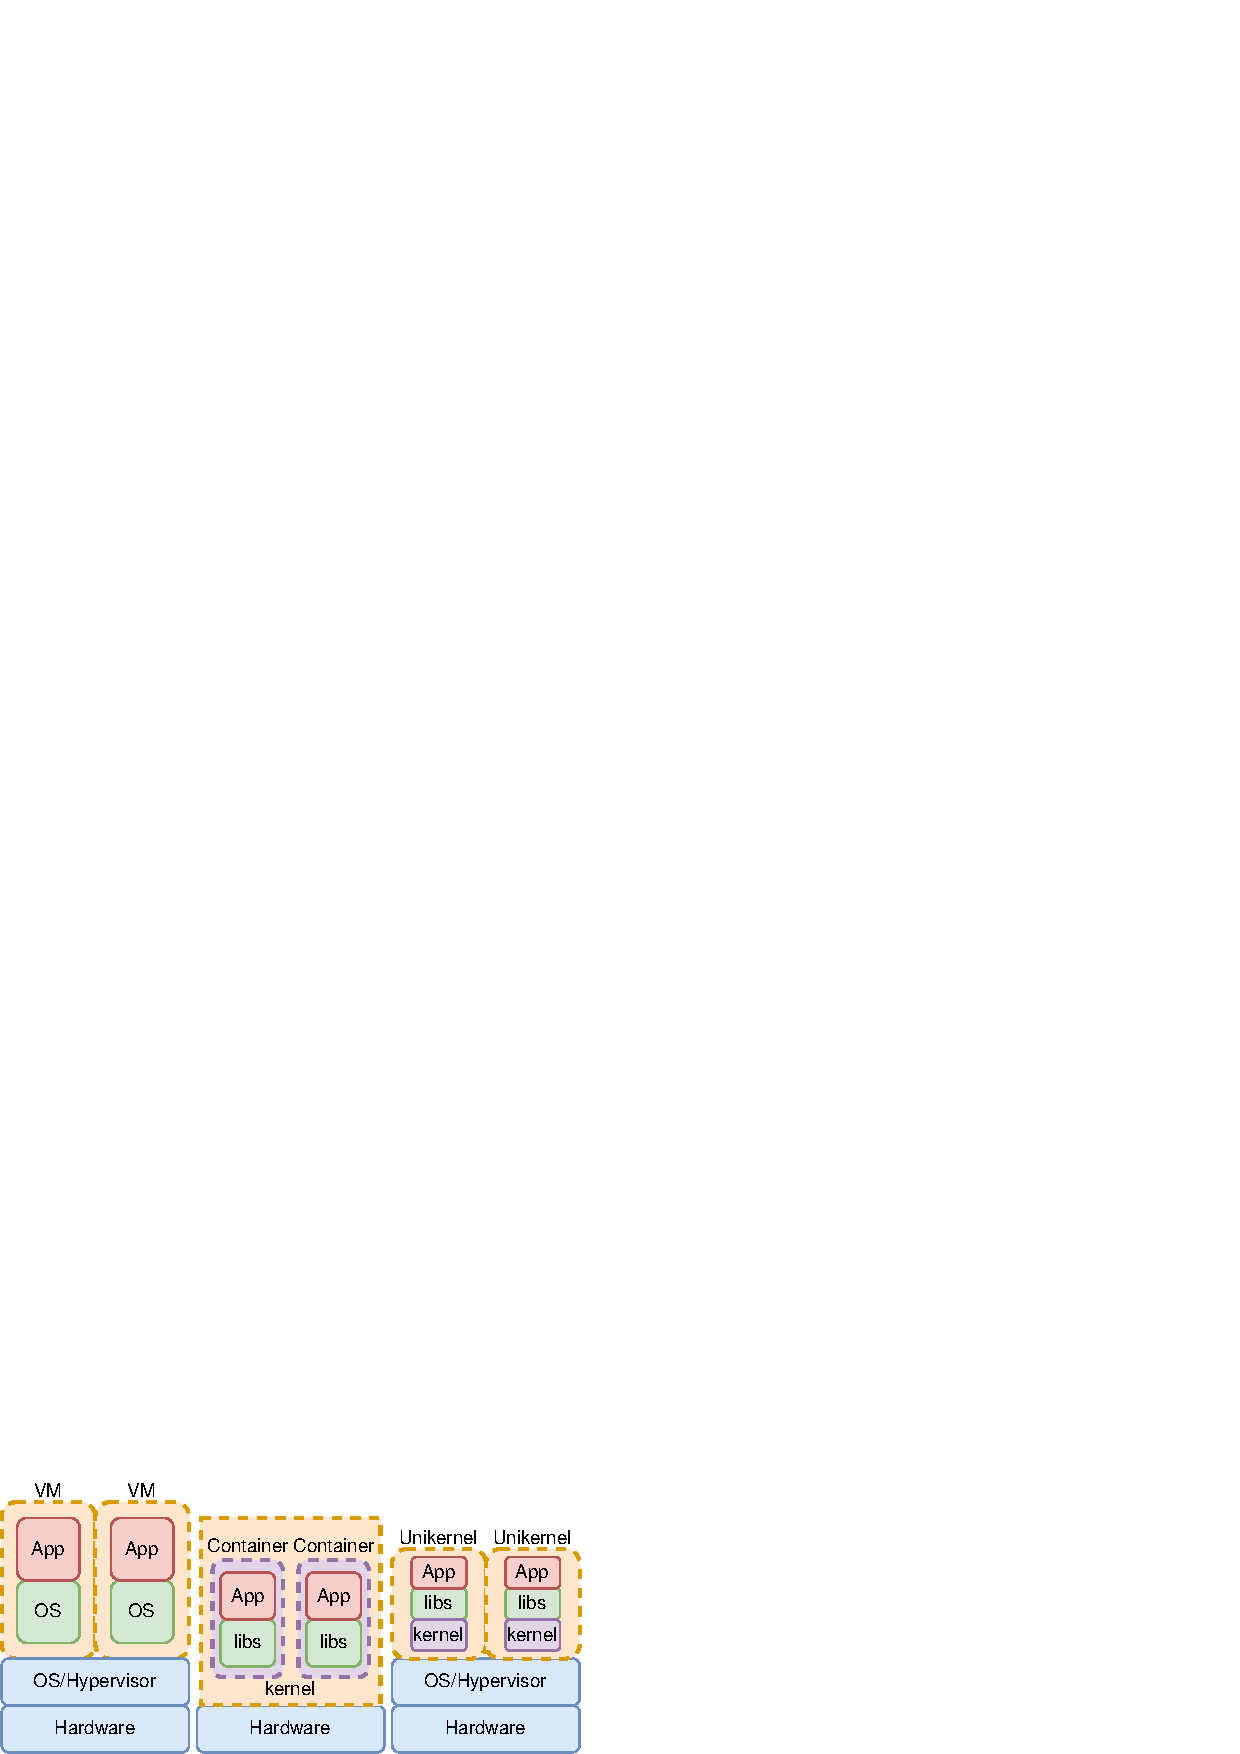
\includegraphics[scale=0.8]{images/Figure5.png}
	\end{center}
	\vspace{-0.6cm}
	\caption{Architectural differences between VMs, containers and unikernels.}
	\label{fig:fig5}
\end{figure}
%
%
\section{Deployment}\label{sec:deployment}
%
Over the years two different approuches evolved how to deploy infrastructure and applications. The difference just get more amplified, when CC and microservices get into the picture, where frequent deployment is very common. 

Here evolve new strategy to mange and deploy complicated infrastructure elements --- Infrastructure as code (IaC). In his book~\cite{wittig2018amazon} Wittig et al. describe it as a process of managing and provisioning computer data centers through machine-readable definition files, rather than physical hardware configuration or interactive configuration tools.

Deplyments in such complex environment can be separated how they handle changes on existing infrastructure or applications on:

\begin{itemize}
	\item \textbf{Mutable model}, is model where we have in place changes which mean that the parts of the existing infrastructure or applications get updated or changed in order to do update. In place change can produce few problems: $(1)$ more risk, beacause in place change my not finish completly which put our infrastructure or the application in possible bad state. This is esspecially probem, if we have a lot of services and multiple copies of the same service. Possibility that our system is not on, is a lot higher, $(2)$ high complexity, this is direct implicatoin of previous feature. Since out change might not get fully done, we can't give guarantis that our infrastructure or applicatoin is transitioned from one version to the another --- change is not \textbf{descrete}, but \textbf{continues} since we might end up in some state in between where we are now and where we want to be.
	\item \textbf{Immutable model}, is model where we do not do any in place changes on existing infrastructure or application whatsoever. In this model, we replace it complety with new version that is updated or changed compared to previous version. Previous version get discarded in favour of new version. Compared to the previous model, immutable deployment have: $(1)$ less risk, since we do not change existing infrastructure or the applicatoin but we start new one with and shut down previous one. This is important esspecially in DS where everyting can fail at any tome, $(2)$ previous property reduce complexity of mutable deployment model. This is direct implicatoin of previous feature, since we shut down and fully replace previous version with new one we get \textbf{descrete} version change and atomic deployment with dafer deployments with fast rollback and recovery processes. On the other hand, this process requre more resources~\ref{Helland16}, since both hersions must be present on the node in order to this process is done. Second problem is data that is used by the app, we should not lost the data that app is generated. If we externalize data than this problems is resolved. We should not rely on local storage, but store that data elsewhere, esspecially when the parts of the system are volatile and changed often. Key adventage of this approuch, is avoiding downtime experienced by the end user when new features are released.
\end{itemize}

Figure~\ref{fig:fig12} summaraze difference bewteen prevous infrastructure deplyment models.

\begin{figure}[H]
	\begin{center}
		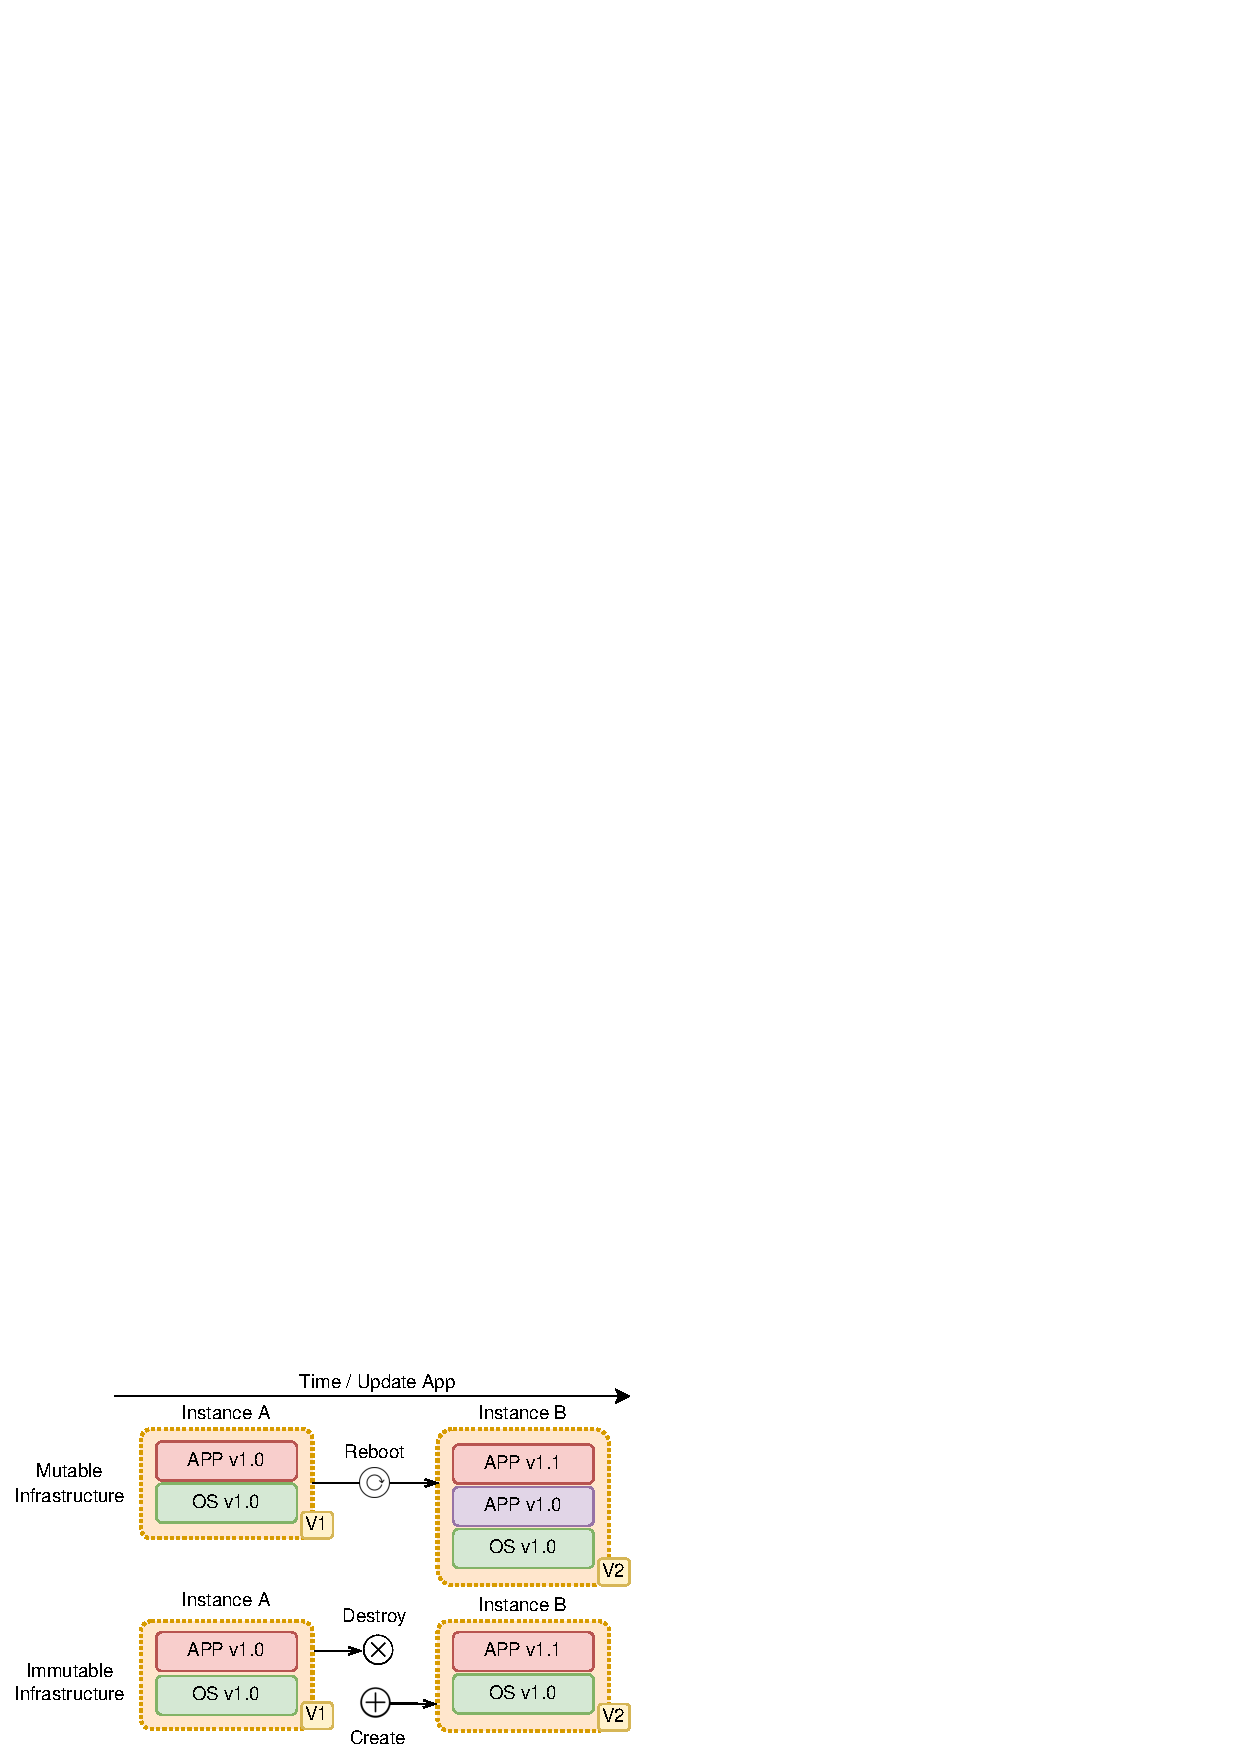
\includegraphics[scale=0.7]{images/Figure12.png}
	\end{center}
	\vspace{-0.6cm}
	\caption{Difference bewteen mutable and immutable deplyment models}
	\label{fig:fig12}
\end{figure}

Immutability is a simple concept to understand, and simplify a lot esspecially in DS~\cite{Helland16}. Write down some data, and ensure that it never changes. It can never be modified, updated, or deleted~\cite{perry2020art}. When this is combined with premisse that we can avoid downtime esspecially in complex DS, it is clear why immutable model is gainign more and more popularity (esspecially with arival of containers). Immutable infrastructure deployment offer few models how to deploy change on the services, even in production to test it, or switch to whole new version. These strategeis include:

\begin{itemize}
	\item \textbf{Blue-Green deployment}, this strategy require two separate environemnts: $(1)$ \textit{Blue} current running version, and $(2)$ \textit{Green} is the new version that needs to be deployed. When we are satisfied that the green version is working properly, we can gradually reroute the traffic from the old environment to the new environment for example by modifying DNS. This strategy offers near zero downtime.
	\item \textbf{Canary update} is the strategy where we do direct a small number of requests to the new version --- the canary. If we are satisfied with the change, we can continue to increase number of requests and monitor how service is working with increasing load, monitor for erros etc.
	\item \textbf{Rolling update} streategy update large environments a few nodes at a time. The setup is similar to blue-green deployment, but here we have single environment. With this strategy, new version gradually replaces the old one. But this is not the only benefit. If for whatever reason, new verrsion is not working properly on larger amount of nodes, we can always do rolling back to previous version.
\end{itemize}

With mutable infrastructure these strategies would be hard to implement, and maybe it is not possible at all. 

Beside infrastructure deployemnt, there is another side that we must consider, and that is how describe these deployments. Here we can consider two different strategies:
\begin{itemize}
	\item \textbf{Imperative}, with this option users have to write code or specific instructions step by step what specific tool need to do in order that application or infrastrucgure is properly setup. In this approuch we have a \textit{smart} user who describe \textit{dumb} machine what is needed to be done and in what order to achieve desired state.
	\item \textbf{Declarative}, with this option user have to describe end state or what is his desired state, and tool needs to figure out the way how to do this. Here we have \textit{smart} system that will found a way how to achieve desired state, and we have user who\textit{do not care} in what order actions need to be done --- that is what system needs to do. User do not need to worry about timing, this simplify whole process and code always represents the latest state. With this type of deployment, we can offer users two different models: $(1)$ use existing formats that are user familiar with like JSON, YAML, XML etc., or $(2)$ create new domain specific language that users need to learn, but we might be able to optimaze description.
\end{itemize}

With introduction of \textit{LinuxKit}, we can create Linux subsystems based around containers, that  are very secure. With linuxkit, every purt of the Linux subsystem is running inside container, so we can assemble a Linux subsystem with services that are needed. As a result, systems created with LinuxKit have a smaller attack surface~\cite{abs-1802-10375} than general purpose systems. This is important from security point of view, but also from infrastructure deployment because we can compose specific OS based around containers that we need for different purpose. And we can update, change and adopt these OS for every machine or purpose we need.

Deployment is based around changeint parts of the OS, and his services that are running inside containers. As a result, everything can be removed or replaced. It's highly portable and can work on desktops, servers, IoT, mainframes, bare metal, and virtualized systems.
%
%
\section{Concurency and parallelism}\label{sec:concurency_parallelism}
%
People usually confuse these two concepts. Even they looks similar, they are different way of doing things. In his talk Rob Pike~\cite{Pike} give great explanation and examples on this topic. In this toke he give great deffinitions of these concepts like:

\begin{itemize}
	\item \textbf{Concurrency} is composition of independently executing things. Concurrency is about dealing with a lot of things at once.
	\item \textbf{Parallelism} is simultaneous execution of multiple things. Parallelism is about doing a lot of things at once. 
\end{itemize}

These things are important, esspecially when building applications and systems that should achieve very high throughput. We must build them with a good structure and a good concurrency model. These features enables possible parallelism, but with communication~\cite{Pike}. These ideas are based on Tony Hoare work of Communicating Sequential Processes (CSP)~\cite{Hoare78}.

\subsection{Actor model}\label{sec:actor_model}
%
In actor model, the main idea is based around \textbf{actors} which are small concurrent code, that communicate independently by sending messages, removing the need for lock-based synchronization~\cite{Hewitt}. This model propose similar idea like Tony Hoare in his work with CSP~\cite{Hoare78}, and actors are oftten confused with CSP. Table~\ref{tab:table6} give differences between actor model and CSP.

\begin{table}[h!]
	\begin{center}
		\begin{tabular}{l|l|l}
			\textbf{Feature} & \textbf{CSP} & \textbf{Actor model}\\
			\hline
			\textbf{Fault tolerance} & Distributed Queue & Hierarchy of supervisors \\
			\textbf{Process identity} & Anonymus & Concrete \\
			\textbf{Composition} & NA & Applicable \\
			\textbf{Communication} & Queue & Direct \\
			\textbf{Message passing} & Sync & Async\\
		\end{tabular}
	\end{center}
	\vspace{-0.5cm}
	\caption{Ddifferences between actor model and CSP.}
	\label{tab:table6}
\end{table}

Actors do not share memory, and they are isolated by nature. Actor can create another actor/s and even watch on them in case they stop unexpectedly. And when an actor finished its job, and he is not needed anymore, it disappears. These actors can create complicated networks that are easy to understand, model and reason about and everything is based on a simple massage passing mechanism. 

Every actor have a designated message box. When a message arrives, actor will test message type and do job acording to message type he received. In this way we are not dependent of lock-based synchronization that can be hard to understand, and it can cause serious problems.

Actor model is fault tolerant by design. It support crush to happend, because there is a \say{self heal} mechanism that will monitor actor/s, and when crash happend it will try to apply some strategy, in most cases just restart actor, but other strategies could be applied. This philosophy is really usefull, because it is hard to think about every single failure option.
%
%
\section{Motivation and Problem Statement}\label{sec:problem_statement}
%
In~\cite{GreenbergHMP09} Greenberg et al. point out that micro data-centers (MDCs) are used primarily as nodes in content distribution networks and other \say{embarrassingly distributed} applications.

One size never fits all, so the cloud should not be our final computing shift. Various models presented in~\ref{sec:mobile_computing}, show possibility that computing could be done closer to the data source, to lower the latency for its clients by contacting the cloud only when needed, while heavy computation remains in the cloud because of resource availability. Send to the cloud only information that is crucial for other services or applications~\cite{inproceedingsSimic1}. Not ingest everything as the standard cloud model proposes.

MDCs with a zone-based server organization is a good starting point for building EC as a service, but we need a more available and resilient system with less latency. EC originates from P2P systems~\cite{LopezMEDHIBFR15} as sugested by L{\'{o}}pez et al., but expands it into new directions and blends it with the CC. But, infrastructure deployment will not happen until the process is trivial~\cite{SatyanarayananBCD09}. Going to every node is tedious and time consuming. Especially when geo-distribution is taken into consideration.

A well defined system could be offered as a service, like any other resource in the CC. We can offer it to researchers and developers to create new human-centered applications. If we need more resources on one side, we can take from one pool of resources and move to another one.
But on the other hand, some CC providers might choose to embed it into their own existing system, hiding unnecessary complexity, behind some communication interface or proposed application model.

The idea of small servers with heterogeneous compute, storage, and network resources, raise interesting research idea and motivation for this thesis. Taking advantage of resources organized locally as micro clouds, community clouds, or edge clouds~\cite{RydenOCW14} suggested by Ryden et al., to help power-hungry servers reduce traffic~\cite{HirschMZ18}. Contact the cloud only when needed~\cite{inproceedingsSimic1}. Send to the cloud only information that is crucial for other services or applications. Not ingest everything as the standard CC model proposes.

To achieve such behavior, dynamic resource management, and device management is essential. We must perceive available resources, configuration, and utilization~\cite{GubbiBMP13, WangZZWYW17}. Traditional DCs is a well organized and connected system. On the other hand, these MDCs consist of various devices, including ones presented in~\ref{sec:mobile_computing} that are not~\cite{JiangCGZW19}. This idea, brings us to the problem this thesis address.

EC and MDCs models lack dynamic geo-organization, well defined native applications model, and clear separation of concerns. As such they cannot be offered as a service to the users. They usually exist independently from one another, scattered without communication between them, offered by providers who mostly lock users in their own ecosystem. Co-located edge nodes should be organized locally, making the whole system and applications more available and reliable, but also extending resources beyond the single node or group of nodes, maintaining good performance to build servers and clusters~\cite{ArocaG12}.

This cloud extension deepens and strengthens our understanding of the CC as a whole. With the separation of concerns setup, EC native applications model, and a unified node organization, we are moving towards the idea of EC as a service. 

Based on this, we define the problem through the following research questions three segments:

\begin{enumerate}[start=1,label={(\bfseries \arabic*)}]
	\item \textit{Can we organize geo-distributed edge nodes in a similar way to the cloud, adopted for the different  environment, with clear separation of concerns and familiar applications model for users.}
	\item \textit{Can we offer these organized nodes as a service to the developers and researchers for new human-centered applications, based on the cloud pay as you go model?}
	\item \textit{Can we make model in such a way that is formaly correct, easy to extend, understand and reason about?}
\end{enumerate}

This cloud-like extension makes the whole system and applications more available and reliable, but also extends resources beyond the single node. Satyanarayanan et al. in ~\cite{SatyanarayananK19} show that MDCs can serve as firewalls, while Simi\' c et al., in~\cite{inproceedingsSimic1} use similar idea as pre-processing tier. At the same time, users are getting a unique ability to dynamically and selectively control the information sent to the cloud. Years after its inception, EC is no longer just an idea~\cite{SatyanarayananK19} but a must-have tool for novel applications to come.
%
%
\section{Research Hypotheses, and Goals}\label{sec:research_hyphotesis_and_golas}
%
Based on reserach questions and motivation presented in~\ref{sec:problem_statement}, we derive the hypotheses around which the thesis is based. It can be summarized as follows:

\begin{enumerate}[start=1,label={(\bfseries \arabic*)}]
	\item \textbf{Hypothesis:} \textit{It is possible to organize EC nodes in a standard way based on cloud architecture, with adaptation for an EC geo-distributed environment. Give users the ability to organize nodes in the best possible way in some geographic areas to serve only the local population in near proximity.}
	\item \textbf{Hypothesis:} \textit{It is possible to offer it to researchers and developers to create new human-centered applications. If we need more resources on one side, we can take from one pool of resources and move to another one, or organize them any other way needed.}
	\item \textbf{Hypothesis:} \textit{It is possible to present clear separation of concerns for the future EC as a service model, and establish a well-organized system where every part has an intuitive role.} 
	\item \textbf{Hypothesis:} \textit{It is possible to present unified model that supports heterogeneous EC nodes, with a set of technical requirements that nodes must fulfil, if they want to join the system.}
	\item \textbf{Hypothesis:} \textit{It is possible to present a clear application model so that users can use full potential of newly created infrastructure.}
\end{enumerate}

From the previously defined hypotheses, we can derive the primary goals of this thesis, where the expected results include:

\begin{enumerate}[start=1,label={(\bfseries \arabic*)}]
	\item \textit{The construction of a model with a clear separation of concerns for the model influenced by cloud organization, with adaptations for a different environment. With a model for EC applications utilizing these adaptations. This addresses the first research question, and is the topic of Chapter~\ref{chapter:Micro_clouds}.}
	\item \textit{The constructed model is more available, resilient with less latency, and as such it can be offered to the general public as a service like any other service in the cloud. This addresses the second research question, and is the topic of Chapter~\ref{chapter:Micro_clouds}.}
	\item \textit{The constructed model is described formaly well, using solid mathematical theory, but also easy to extend both formaly and technicaly, easy to understand and reason about. This addresses the third research question, and is the topic of Chapter~\ref{chapter:Micro_clouds}.}
\end{enumerate}
%
%
\section{Structure of the thesis}\label{sec:structure_of_thesis}
%
Throughout this introductory Chapter, we defined the motication for out work with problems that this thesis addresses and presented the necessary background informations and areas to support our work. Here we outline the rest of the thesis.

Chapter~\ref{chapter:Review} presents the literature review, where we examine different aspects of existing systems and methods important for the thesis. We analyze existing nodes organizational abilities in both industry and academia frameworks and solutions to address our first research question. We further exemine platform models from industry and academia tools and frameworks to address our second research question. And last but not least, we examine current strategies to offload tasks from the cloud. All three parts address our third research question.

Chapter~\ref{chapter:Micro_clouds} details our model, how it is related to other research and where it connects to other existing models and solutions. We further describe our solution as well as protocols requried for such sysrtem to be implemented foramly. We give examples of how exisintg infrastructure could be used, as well as familiar application model for developers. 

Chapter~\ref{chapter:Implementation} present implementation details of an framework developed to test hypotheses defined earlier in this chapter, but also model and foramly defined protocols defined in~\ref{chapter:Micro_clouds}. This chapter also show results after conducting experiments, current limitations of implemented system, and possible applications that could benefit from such system.

Chapter~\ref{chapter:Conclusion} concludes our work and presents opportunities for further research and development.
%
%
%!TEX root =  main.tex
\chapter{Field review}\label{chapter:Field_overview}
%
An overview of the topics that are of significant importance for the rest of the thesis is going to be given in this section, since the thesis is heavily based on these topics. 

Sections~\ref{sec:distributed_systems} and \ref{sec:distributed_computing} describe the theoretical background behind the problem, where we examine distributed systems (DS) and distributed computing (DC), focusing on design details, communication patterns, and organizational structure. Section~\ref{sec:similar_models} describes similar models that might be a source of confusion, and how they are different than DS or DC, and how some concepts can fit in the bigger picture. Section~\ref{sec:transactions} describes different transaction models used for different applications. Section~\ref{sec:garbage_collection} describes basics of garbage collection techniques and why it is important. Section~\ref{sec:virtualization_techniques} describes different virtualization methods that are used in CC for systems and/or applications. Section~\ref{sec:deployment} describes different architecture and application model and how deployment can be done in large DS. Section~\ref{sec:ias} describes infrastructure as software model that allows abstracting infrastructure to software level. Section~\ref{sec:dev_roles} describes different development roles in the modern complex software environment, with focus on technical roles, while Section~\ref{sec:concurency_parallelism} describes the difference between concurrency and parallelism and introduces an actor system, that will be used later on in the thesis. 

\section{Distributed systems}\label{sec:distributed_systems}
%
There are various definitions of DS, but we can think of DS as a system where multiple entities can communicate to one another in some way, but at the same time, they can perform some operations. In~\cite{SteenT16, 0019513} Tanenbaum et al. give two interesting assumptions about DS:

\begin{enumerate}[start=1,label={(\bfseries \arabic*)}]
	\item  \say{A computing element, which we will generally refer to as a node, can be either a hardware device or a software process}.
	\item \say{A second element is that users (be they people or applications) believe they are dealing with a single system. This means that one way or another the autonomous nodes need to collaborate}.\label{ds:asumption_2}
\end{enumerate}

\noindent
These two assumptions are useful and powerful when talking about DS. As such, in this thesis, we will adopt and use them rigorously.

Three significant characteristics of distributed systems are~\cite{0019513}: 

\begin{enumerate}[start=1,label={(\bfseries \arabic*)}]
	\item \textbf{concurrency of components}, refers to the ability of the DS that multiple activities are executed at the same time. These activities take place on multiple nodes that are part of a DS.
	\item \textbf{independent failure of components}, this property refers to a nasty feature of DS that nodes fail independently. They can fail at the same time as well, but they usually fail independently for numerous reasons.
	\item \textbf{lack of a global clock}, this is a consequence of dealing with independent nodes. Each node has its notion of time, and as such we cannot assume that there is something like a global clock.
\end{enumerate} 

\noindent
In~\cite{SteenT16} authors give formal definition \say{distributed system is a collection of autonomous computing elements that appears to its users as a single coherent system}.

When talking about DS, we usually think about computing systems that are connected via network or over the internet. But DS is not exclusive to the domain of computer science. They existed before computers started to enrich almost every aspect of human life. DS have been used in various different domains such as: \textbf{telecommunication networks}, \textbf{aircraft control systems}, \textbf{industrial control systems} etc. DS are used anywhere where the number of users is growing rapidly so that a single entity cannot respond to the demands in (near) real-time.

Distributed systems (in computer science) consist of various algorithms, techniques, and trade-offs to create an illusion that a set of nodes act as one. Algorithms and techniques used in the DS may include the following: \textbf{(1)} replication, \textbf{(2)} consensus, \textbf{(3)} communication, \textbf{(4)} storage,\textbf{(5)} processing, \textbf{(6)} membership, \textbf{(7)} scheduling etc.

DS are hard to implement because of their asinchroninis and faulty nature. James Gosling and Peter Deutsch both fellows at Sun Microsystems at the time created a list of problems for network applications known as \textit{8 fallacies of Distributed Systems}:\label{enum:fallacies}

\begin{enumerate}[start=1,label={(\bfseries \arabic*)}]\label{ds:8_fallacies}
	\item \textbf{The network is reliable}; there will always be something that goes wrong with the network --- power failure, a cut cable, environmental disasters, etc.
	\item \textbf{Latency is zero}; locally latency is not an issue, but it deteriorates very quickly when you move to the internet and CC scenarios;
	\item \textbf{Bandwidth is infinite}; even though bandwidth is constantly getting better and better, the amount of data we try to push through it rise as well.
	\item \textbf{The network is secure};  Internet attack trends are showing growth, and this becomes a problem even more in public CC;
	\item \textbf{Topology doesn't change}; network topology is usually out of user control, and network topology changes constantly for numerous reasons --- added or removed new devices, servers, breaks, outages, etc;
	\item \textbf{There is one administrator}; nowadays there are numerous administrators for web servers, databases, cache and so on, , and companies collaborate with other companies or CC providers;
	\item \textbf{Transport cost is zero}; we have to serialize information and send data over the wire, which takes resources and adds to the total latency. The problem here is not just latency, but that information serialization takes time and resources;
	\item \textbf{The network is homogeneous}; today, a homogeneous network is the exception, rather than a rule. We have different servers, systems, clients that interact. The implication of this is that we have to assume interoperability between these systems sooner or later, which we must be aware of. We might also have some proprietary protocols that might also take time to send on and they may stay without support, so we should avoid them.
\end{enumerate}

\noindent
These fallacies were introduced over a decade ago, and more than four decades since we started building DS, but the characteristics and underlying problems remain pretty the same. An interesting fact is that even designers, architects still assume that technology solves everything. This is not the case in DS, and these fallacies should not be forgotten. Because of these problems, DS are hard to implement correctly and they are hard to maintain and test properly.
%
%
\subsection{Scalability}\label{sec:scalability}
%
Scalability is the property of a system to handle a growing amount of work by adding resources to the system~\cite{Bondi00}. When talking about computer systems, scalability can be represented in two ways:

\begin{itemize}
	\item \textbf{Scaling vertically} means upgrading the hardware that computer systems are running on --- adding mode CPU, RAM, storage. Vertical scaling can increase performance to what the latest hardware can offer, and here we are limited by the laws of physics and Moor's law \cite{Gustafson2011}. A typical example that requires this type of scaling is a relation database server. These capabilities are insufficient for moderate to big workloads.
	\item \textbf{Scaling horizontally} means that we scale our system by adding more and more computers, rather than upgrading the hardware of a single one. With this approach, we are (almost) limitless on how much we can scale. Whenever performance degrades we can simply add more computers (or nodes). These nodes are not required to be some high-end machines.
\end{itemize}

\noindent
Figure~\ref{fig:fig23} show difference betweeen scaling vertically and horizontally.

\begin{figure}[H]
	\begin{center}
		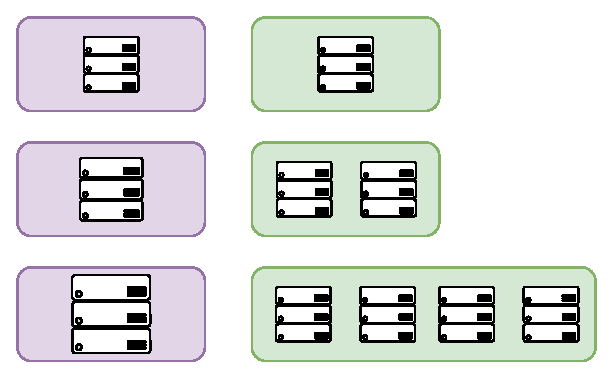
\includegraphics[scale=0.80]{images/Figure23}
	\end{center}
	\vspace{-0.6cm}
	\caption{Difference betweeen scaling vertically and horizontally}
	\label{fig:fig23}
\end{figure}

\noindent
Table~\ref{tab:table1} summarizes differences between horizontall and verticall scaling.

\begin{table}[h!]
	\begin{center}
		\begin{tabular}{l|l|l}
			\textbf{Feature} & \textbf{Scaling vertically} & \textbf{Scaling horizontally}\\
			\hline
			\textbf{Scaling} & Limited & Unlimited \\
			\textbf{Managment} & Easy & Comlex\\
			\textbf{Investments} & Expensive & Afordable \\
		\end{tabular}
	\end{center}
	\vspace{-0.5cm}
	\caption{Differences between horizontal and vertical scaling.}
	\label{tab:table1}
\end{table}

\noindent
Scaling horizontally is a preferable way for scaling DS. Not because we can scale easier, or because it is significantly cheaper than vertical scaling (after a certain threshold)~\cite{Bondi00}, but because this approach comes with few more benefits that are especially important when talking about large-scale DS. Adding more nodes gives us two important properties: 

\begin{itemize}
	\item \textbf{Fault tolerance} means that applications running on multiple places at the same time are not bound to the fail of a node, cluster, or even DCs. As long as there is a copy of the application running somewhere, the user will get a response back. As a consequence of running multiple copies of a service and on multiple places, we have that service is more \textbf{available}, than running on a single node no matter how high-end that node is. Eventually, all nodes are going to break, and if we have multiple copies of the same service we have a more resilient and more available system to serve user requests.
	\item \textbf{Low latency} refers to the idea that the world is limited by the speed of light. If a node running application is too far away, the user will wait too long for the response to get back. If the same application is running in multiple places, the user request will hit the node that is closest to the user.
\end{itemize}

\noindent
Nodes are usually organized into clusters of machines. Buyya et al. describes a cluster as a processing system, which consists of a collection of interconnected stand-alone computers cooperatively working together as a single, integrated computing resource.~\cite{Buyya}.

But despite all the obvious benefits, for a DS to work properly, we need the writing software in such a way that is able to run on multiple nodes, as well as that it \textbf{accepts the failure and deals with it}. This turns out to be not an easy task.

For example, users need to be aware when using DS which of them is related to distributed data storage systems. Storage implementations that rely on vertical scaling to ensure scalability and fault tolerance, have one nasty feature. 

This nasty feature is represented in theorem called \textbf{CAP theorem}~\label{lab:cap} presented by Eric Brewer~\cite{Brewer2000}, and proven after inspection by Gilbert et a.~\cite{GilbertL02}. The CAP theorem states that it is impossible for a distributed data store to simultaneously provide more than two out of three guarantees shown in Figure~\ref{fig:fig17}.

\begin{figure}[H]
	\begin{center}
		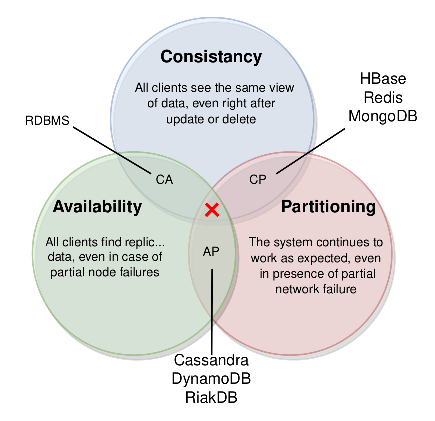
\includegraphics[scale=0.85]{images/Figure17}
	\end{center}
	\vspace{-0.6cm}
	\caption{Difference between cloud options and on-premises solution.}
	\label{fig:fig17}
\end{figure}

\begin{enumerate} [start=1,label={(\bfseries \arabic*)}]
	\item \textbf{C}onsistency, which means that all clients will see the same data at the same time, no matter which node they are connected to. Clients may not be connected to the same node since data could be replicated on many nodes in different locations.
	\item \textbf{A}vailability, which means that any client issued request will get a response back, even if one or more nodes are down. DS will not interpret this situation as an exception or error. Availability is represented in percentage, and it describes how much downtime is allowed per year. This can be calculated using formula:\\ 
	
	\begin{equation}\label{eq:Availability}
	Availability = \frac{uptime}{ (uptime + downtime)}
	\end{equation}
	\myequations{Availability percentage formula}
	The industry is using measuring availability in \say{class of nines}. Availability class is the number of leading nines in the availability figure for a system or module~\cite{GrayS91}. This metric relates to the amount of time (per year) that service is up and running. Table~\ref{tab:table7} show different classes of nine and their availability and unavailability in minutes per year (\textbf{min/year}) for some examples~\cite{GrayS91}.
	
	\begin{table}[h!]
		\begin{center}
			\begin{tabular}{l|l|l}
				\textbf{Type} & \textbf{Availability} & \textbf{Unavailability} \\
				\hline
				\textbf{Unmanaged} & 90\% & 50,000 \\
				\textbf{Managed} & 99\% & 5,000 \\
				\textbf{Well-managed} & 99.9\% & 500 \\
				\textbf{Well-managed} & 99.9\% & 500 \\
				\textbf{Fault-tolerant} & 99.99\% & 50 \\
				\textbf{High-availability} & 99.999\% & 5 \\
				\textbf{Very-high-availability} & 99.9999\% & 0.5 \\
			\end{tabular}
		\end{center}
		\vspace{-0.5cm}
		\caption{Downtime for different classes of nines.}
		\label{tab:table7}
	\end{table}
	
	\noindent
	We can calculate availability class if we have system availability $A$, the system's availability class is defined as~\cite{GrayS91}: 
	
	\begin{equation} 
	e^{\log_{10} \frac{1}{ (1 - A)}} 
	\end{equation}
	\myequations{Availability class formula.}
	It is important to notice that even a 99\% available system gives almost four days of downtime in a year, which is unacceptable for services like Facebook, Google, AWS, etc. And when the service is down, companies are losing customers.
	\item \textbf{P}artition tolerance, which means that the cluster must continue to work despite any number of communication breakdowns between nodes in the system. It is important to state that in a distributed system, partitions cannot be avoided.
\end{enumerate}

\noindent
Years after CAP theorem inception, Shapiro et al. prove that we can alleviate CAP theorem problems, but only in some cases, and offers \textbf{Strong Eventual Consistency (SEC) model}~\cite{ShapiroPBZ11}. They prove that if we can represent our data structure to be: \label{crdts}

\begin{itemize}
	\item \textbf{Commutative} $a*b = b*a$ \myequations{Commutative formula.}
	\item \textbf{Associative} $(a*b)*c = a*(b*c)$ \myequations{Associative formula.}
	\item \textbf{Idempotent} $(a * a) = a$ \myequations{Idempotent formula.}
\end{itemize}

\noindent
where $*$ is a binary operation, for example: $max$, $union$, $or$ we can rely on SEC properties,
%
%
\subsection{Cloud computing}\label{sec:cloud_computing}
%
Vogels et al. describe CC as an \say{aggregation of computing resources as a utility, and software as a service}~\cite{Vogels}.  Big DCs provide hardware and software services for their users over the internet~\cite{AboveTheCloud}. Cloud providers offer various resources like CPU, GPU, storage, and network as utilities that can be used and released on-demand~\cite{ZhangCB10}. 

The key strength of the CC is reflected in the offered services~\cite{Vogels}. To support the various application needs, the traditional CC model provides enormous computing and storage resources elastically. This property refers to the cloud ability to allow services to allocate additional resources or release unused ones to match the application workloads on-demand~\cite{AssuncaoVB18}. 

Services usually fall in one of three main categories: 

\begin{itemize}
	\item \textbf{Infrastructure as a service (IaaS)} allows businesses to purchase resources on-demand and as-needed instead of buying and managing hardware themselves;
	\item \textbf{Platform as a service (PaaS)} delivers a framework for developers to create, maintain and manage their applications. All resources are managed by the enterprise or a third-party vendor;
	\item \textbf{Software as a service (SaaS)} delivers applications over the internet to its users. These applications are managed by a third-party vendor;
\end{itemize}

\noindent
Figure~\ref{fig:fig1} shows the difference in control and management of resources between different cloud options and on-premises solutions.

\begin{figure}[H]
	\begin{center}
		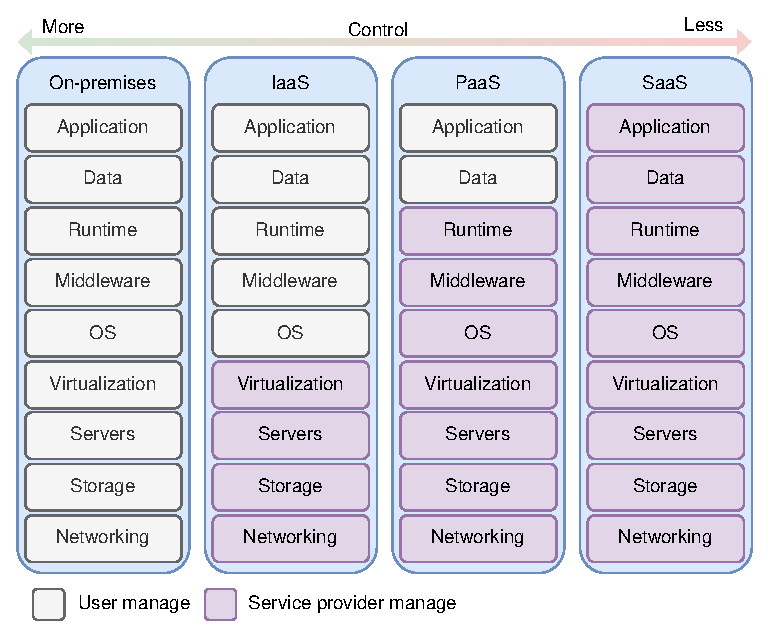
\includegraphics[scale=0.75]{images/Figure1}
	\end{center}
	\vspace{-0.6cm}
	\caption{Difference between cloud options and on-premises solution.}
	\label{fig:fig1}
\end{figure}

\noindent
The user can choose a single solution, or combine more of them if such a thing is required depending on preferences and needs.

By the ownership, CC can be categorized into three categories:

\begin{itemize}
	\item \textbf{Public cloud} is a type where CC is delivered over the internet and shared across many many organizations and users. In this type of CC, architecture is built and maintained by others. Users and organizations pay for what they use. Examples include AWS EC2, Google App Engine, Microsoft Azure, etc.
	\item \textbf{Private cloud} is a type where CC is dedicated only to a single organization. In this type of CC, architecture is built by an organization that may offer their solution or services to the users or other organizations. These services are in the domain of what the organization does, and that organization is in charge of maintenance. Examples include VMWare, XEN, KVM, etc.
	\item \textbf{Hybrid cloud} is such an environment that uses both public and private clouds. Examples include IBM, HP, VMWare vCloud, etc.
\end{itemize}

\noindent
Table~\ref{tab:table4} shows comparison of public, private and hybrid cloud capabilities.\label{sec_types}

\begin{table}[h!]
	\begin{center}
		\begin{tabular}{l|l|l|l}
			\textbf{Capabilities} & \textbf{Public cloud} & \textbf{Private cloud} & \textbf{Hybrid cloud}\\
			\hline
			\textbf{Data control} & IT enterprise & Service Provider & Both \\
			\textbf{Cost} & Low & High & Moderate \\
			\textbf{Data security} & Low & High & Moderate \\
			\textbf{Service levels} & IT specific & Provider specific & Aggregate \\
			\textbf{Scalability} & Very high & Limited & Very high \\	
			\textbf{Reliability} & Moderate & Very high & Medium/High\\	
			\textbf{Performance} & Low/Medium & Good & Good \\
		\end{tabular}
	\end{center}
	\vspace{-0.5cm}
	\caption{Comparison of public, private and hybrid cloud capabilities.}
	\label{tab:table4}
\end{table}

\noindent
In the rest of the thesis, if not stated differently when CC term is used it denotes public cloud.

CC has been the dominating tool in the past decade in various applications~\cite{Satyanarayanan17}. It is changing, evolving, and offering new types of services. Resources such as container as a service (CaaS), database as a service (DBaaS)~\cite{Peter} are newly introduced. The CC model gives us a few benefits. Centralization relies on the economy of scale to lower the cost of administration of big DCs. Organizations using cloud services avoid huge investments, like creating and maintaining their own DCs. They consume resources usually created by others~\cite{Satyanarayanan17} and pay for usage time -- pay as you go model. 

Centralization gives us a few really hard problems to solve. As already stated in section~\ref{sec:problem_area} data is required to be moved to the cloud from data sources, which introduces a high latency in the system~\cite{HossainRH18}. 

There are a few notable attempts to help data ingestion into the cloud. Remote Direct Memory Access (RDMA) protocol makes it possible to read data directly from the memory of one computer and write that data directly to the memory of another. This is done by using \textit{specialized hardware} interface cards and switches and software as well, and operations like read, write, send, receive, etc. do not go through the CPU. With these characteristics, RDMA has low latencies and overhead, and as such reaches better throughputs~\cite{CohenTKCKRCDG09}. This new hardware may not be cheap, and not every CC provider uses them for every use-case. This may not be enough, especially with the ever-growing amount of IoT devices and services.

Over the years there are more service options available, forming \textbf{everything as a service (XaaS)} model~\cite{DuanFZSNH15}. This model proposes that any hardware or software resource can be offered as a service to the users over the internet.

Table~\ref{tab:table2} shows common examples of SaaS, PaaS, and IaaS applications.

\begin{table}[h!]
	\begin{center}
		\begin{tabular}{l|l}
			\textbf{Platform} & \textbf{Common Examples}\\
			\hline
			\textbf{IaaS} & AWS, Microsoft Azure, Google Compute Engine \\
			\textbf{PaaS} & AWS Elastic Beanstalk, Azure, App Engine \\
			\textbf{SaaS} & Gmail, Dropbox, Salesforce, GoToMeeting \\
		\end{tabular}
	\end{center}
	\vspace{-0.5cm}
	\caption{Common examples of SaaS, PaaS, and IaaS.}
	\label{tab:table2}
\end{table}

\subsubsection{Multi-cloud and sky computing}
%
In recent years there has been one extension of CC from a series standpoint called \textbf{multi-cloud}~\cite{HongDSH19, Ardagna15} or sky computing~\cite{StoicaS21} (terms are going to be used interchangeably). 

It is such an environment where an enterprise uses more than one cloud platform, with at least two or more public cloud providers that each delivers a specific application or service. 

A multi-cloud can be comprised of any model presented on page~\pageref{sec_types}. This model relies on the possibility that if one cloud provider fails for whatever reason, the next one will be able to serve user requests.

This strategy allows creation of a single heterogeneous architecture, allowing distribution of cloud assets and workloads across multiple providers (active-active), or deploy a single workload on one provider, with a backup on another (active-passive)~\cite{Multicloud2019}.

CC gives a user an illusion that he is using a single machine, while the background implementation is fairly complicated and consists of various elements that are composed of countless machines. CC is a typical example of a horizontally scalable system presented in~\ref{sec:scalability}.
%
%
\subsection{Membership protocol}\label{sec:memership_protocol}
%
At the beginning of this section DS were introduced, and two interesting assumptions by Tanenbaum et al. were presented~\cite{SteenT16, 0019513}. If one more look is taken at~\ref{ds:asumption_2} assumption, we will see that users of the DS whether they are users or applications perceive DS as a single unit. Inside this single unit, nodes need to collaborate, so that they are able to do various kinds of tasks.

The most basic of all these tasks is that nodes need to know which group they belong to, and who are their peers in the group they will collaborate with. This might sound like a trivial idea, but when we include 8 fallacies of the DS~\ref{ds:8_fallacies} into the equation, things start to be not so trivial after all. In the setup where nodes are connected over the local network or internet, and they need to communicate, things will go wrong for various reasons.

To resolve the problem who their group peers are, a membership protocol comes to help. These protocols need to ensure that each process of one group updates its local list of \textbf{non-faulty} members of the group, and when a new process joins or leaves the group, the local list for every process needs to be updated. This is the most basic idea behind membership protocols.

Processes in the group of nodes in a group will ping each other in different ways, and using different strategies to figure out which nodes are dead and which are alive. There are a few existing algorithms that do this job, and they are (usually) based on the way epidemics spread or how gossip is spread in a human population. Because of this feature, these algorithms are usually called \textit{Gossip} style protocols.

Every membership protocol has some properties that will ensure efficiency and scalability:

\begin{enumerate}[start=1,label={(\bfseries \arabic*)}] \label{ds:features}
	\item \textbf{Completeness}, this property must ensure that every failure in the system is detected.
	\item \textbf{Accuracy}, in an ideal world, there should be no mistakes when detecting failures, but In a real-life scenario, we need to reduce false positives as much as we can.
	\item \textbf{Failure detection speed}, all failures needs to be treated as fast as possible, in order to remove the node from the group and reschedule the tasks from the dead node to alive ones.
	\item \textbf{Scale}, with this property we must ensure that the network load that is generated should be distributed equally between all processes in the group.
\end{enumerate}

\noindent
The easiest idea to implement this protocol would be \textbf{heartbeating} technique where process $P_i$ will send a heartbeat message to all his peers in the group or \textbf{multicast}. After some time if process $P_j$ did not receive a heartbeat message from $P_i$, it will mark him as failed. This idea is easy to understand, and implement but the downsides are that its process is not that \textbf{scalable}, especially for large groups, and this will introduce huge network traffic.

To resolve this problem, Das et al.~\cite{DasGM02} introduced \textbf{S}calable \textbf{W}eakly-consistent \textbf{I}nfection-style Process Group \textbf{M}embership protocol\newline (\textbf{SWIM} for short)\label{swim}. 
\noindent
This protocol divides the membership problem into two parts:

\begin{enumerate}[start=1,label={(\bfseries \arabic*)}]
	\item \textbf{Failure detection}, this component works so that one node will select a random node in the group, and it will send it $ping$ message, expecting $ack$ message in return --- \textbf{direct ping}. If such message is not received, it will pick $n$ nodes to probe through a $ping-req$ message --- \textbf{indirect ping}. If this fails, the node will be marked as $suspected$, and it will be marked as $dead$ after some timeout. If the node gets alive, it will ping some other node and it will get back into the group. Figure~\ref{fig:fig15} show message passing in \textbf{direct} $(left)$, and \textbf{indirect} $(right)$ ping in SWIM protocol.
	\item \textbf{Information dissemination}, with previous strategy, information can be disseminated by \textbf{piggybacking} the data on multiple messages ($ping$, $ping-req$ and $ack$), and avoid using the multicast solution.
\end{enumerate}

\begin{figure}[H]
	\begin{center}
		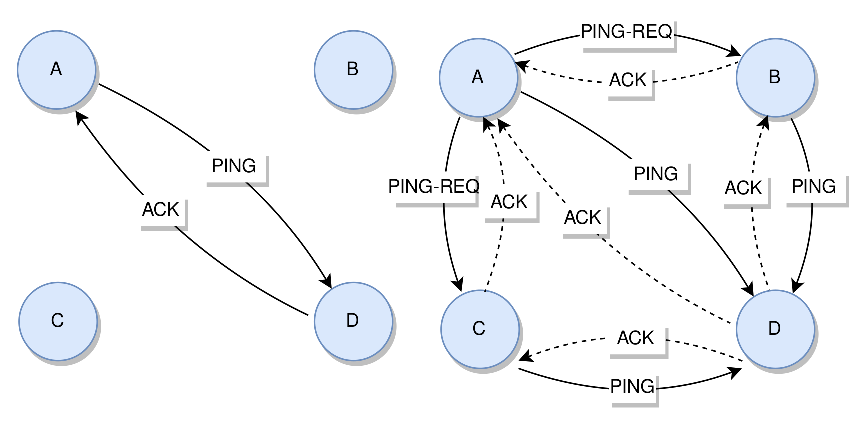
\includegraphics[scale=0.7]{images/Figure15}
	\end{center}
	\vspace{-0.6cm}
	\caption{Direct and indirect ping in SWIM protocol.}
	\label{fig:fig15}
\end{figure}

\noindent
Over the years, researchers found ways to improve the protocol, for example Dadgar et al. presented \textit{Lifeguard protocol}~\cite{DadgarPC18} for more accurate failure detection, and there are other implementations to fine-tune the SWIM, but the base idea is still there. Today SWIM or SWIM-like protocols are standard membership protocols whenever some node clustering is done.
%
%
\subsection{Mobile computing}\label{sec:mobile_computing}
%
The first idea that introduced task offloading from the cloud~\cite{FernandoLR13, LinLJL19} was Mobile cloud computing (MCC). Mobile devices run small client software and interact with the cloud over the internet, while heavy computation remains in the cloud. 

The cloud is usually far away from end devices because DCs are built on specific locations in the world to target as many users nearby as possible. This sparse deployment will most likely lead to high latency, and bad quality of experience (QoE)~\cite{LinLJL19} for most users. Latency-sensitive applications especially will have a hard time. As a model, MCC is not much different from the standard CC model. The good thing is that the cloud has been relaxed a little bit, and a small number of tasks has been moved from the cloud. But this model opens the door for the next-generation models.

The development led to new computing areas like EC, osmotic computig~\cite{VillariFDRJR19, VillariCF17}, sky computing~\cite{StoicaS21}, etc. EC is a next-generation model where computing and storage resources are in proximity to data sources~\cite{Satyanarayanan17}. This idea might overcome cloud latency issues and known MCC problems. The main strength of the EC lays in the CC enhancements with new processing ideas, for the next-generation use-cases~\cite{NingLSY20}. 

EC has brought a few different models over the years. Models like fog~\cite{BonomiMNZ14}, cloudlets~\cite{MonsalveCC18}, and mobile edge computing (MEC)~\cite{WangZZWYW17} emerged. This thesis will refer to all these models as edge nodes. Different EC models rely on the concept of data and computation offloading from the cloud closer to the ground~\cite{KhuneP19}. Only heavy computation remains in the cloud because of more available resources~\cite{NingLSY20}, compared to edge nodes. 

EC models introduced small-scale servers that operate between data sources and the cloud. These small-scale servers have much fewer capabilities compared to the cloud servers~\cite{ChenHLLW15}. To avoid latency and huge bandwidth~\cite{MonsalveCC18}, EC nodes can be dispersed in various locations, for example, base stations~\cite{WangZZWYW17}, coffee shops, or over arbitrary geographic regions.
%
%
\section{Distributed computing}\label{sec:distributed_computing}
%
Distributed computing (DC) can be defined as the use of a DS to solve one large problem by breaking it down into several smaller parts, where each part is computed in the individual node of the DS and coordination is done by passing messages to one another~\cite{0019513}. Computer programs that use this strategy and run on DS are called \textbf{distributed programs} \cite{Vera16, andrews2000foundations}. 

Similar to CC in Section~\ref{sec:cloud_computing}, to a normal user, DC systems appear as a single system similar to one the user uses every day on his/her personal computer. DC shares the same fallacies to DS presented in~\ref{sec:distributed_systems}.
%
%
\subsection{Big Data}\label{sec:big_data}
%
Term big data means that the data is unable to be handled, processed, or loaded into a single machine~\cite{FisherDCD12}. That means that traditional data mining methods or data analytics tools developed for centralized processing may not be able to be applied directly to big data~\cite{Tsai2015}. 

New tools and methods that have been developed rely on DS and one specific feature \textbf{data locality}~\label{ds:data_locality}. Data locality can be described as a process of moving the computation closer to the data, instead of moving large data to computation~\cite{GuoFZ12}. This simple idea minimizes network congestion and increases the overall throughput of the system.

Two examples of how huge generated data could be have already been given in~\ref{sec:problem_area}, and when other IoT sensors and devices are included these numbers will just keep getting bigger and bigger~\cite{SarigiannidisLR20}.

Contrary to relational databases that mostly deal with structured data, Big Data is dealing with various kinds of data~\cite{FisherDCD12, Tsai2015, GuoFZ12}:

\begin{itemize}
	\item \textbf{Structured} data is a kind of data that have some fixed structure and format. A typical example of this is data stored inside a table of some database. Organizations usually have no huge problem extracting some kind of value out of the data.
	\item \textbf{Unstructured} data is a kind of data where there is not any kind of structure at all. These data sources are heterogeneous and may contain a combination of simple text files, images, videos, etc. This type of data is usually in raw format, and organizations have a hard time deriving the value out.
	\item \textbf{Semi-structured} data is the kind of data that can contain both previously mentioned types of data. An example of this type of data is XML files.
\end{itemize}

\noindent
Along with the share size, big data have other instantly recognizable features called \textbf{V's} of big data~\cite{PatgiriA16}. 

The name is derived from initial letters of the other features that are describing big data. 

Image~\ref{fig:fig3} show 6 V's commonly used to represent the big data.

\begin{figure}[H]
	\begin{center}
		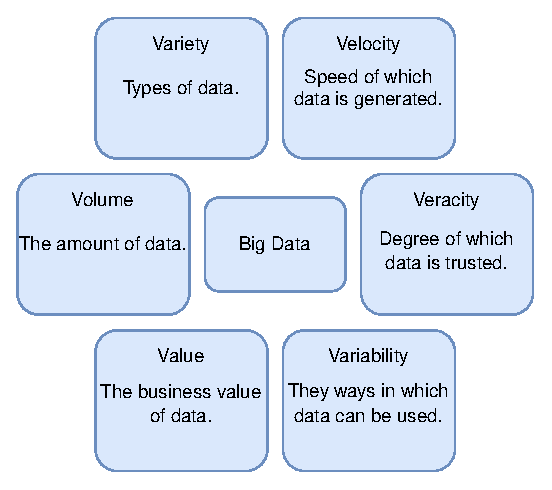
\includegraphics[scale=0.7]{images/Figure3}
	\end{center}
	\vspace{-0.6cm}
	\caption{V's of Big Data.}
	\label{fig:fig3}
\end{figure}

\noindent
Processing in big data systems can be represented as~\cite{phdthesis, KiranMMDB15}:

\begin{itemize}
	\item \textbf{Batch processing} represents a data processing technique that is done on a huge quantity of the stored data. This type of processing is usually slow and requires time.
	\item \textbf{Stream processing} represents a data processing technique that is done as data get into the system. This type of processing is usually done on a smaller quantity of the data \textbf{at the time}, and it is faster.
	\item \textbf{Lambda architectures} represents a processing technique where stream processing and handling of massive data volumes in a batch are combined in a uniform manner, reducing costs in the process~\cite{KiranMMDB15}.
\end{itemize}

\noindent
Big data systems, are not processing and value extracting systems. Big data systems can be separated into several categories: \textbf{(1)} data storage, \textbf{(2)}, data ingestion \textbf{(3)}, data processing, and analytics. All these systems aid to properly analyze ever-growing requirements~\cite{RaoMBG19},

Despite a promise that big data offers to derive value out of the collected data, this task is not easy to do and requires a properly set up system filtering and removing data that contains no value. To aid this idea, data could be filtered and a little bit preprocessed on close to the source~\cite{inproceedingsSimic1}, and as such sent to data lakes~\cite{MarynowskiSP15}.
%
%
\subsection{Microservices}\label{sec:microservices}
%
There is no single comprehensive definition of what a microservice is. Different people and organizations use different definitions to describe it. A working definition is offered in~\cite{DragoniGLMMMS16} as~\say{a microservice is a cohesive, independent process interacting via messages}. Despite the lack of a comprehensive definition, all agree on a few features that come with microservices:

\begin{enumerate}[start=1,label={(\bfseries \arabic*)}]
	\item they are small computer programs that are independently deployable and developed.
	\item they could be developed using different languages, principles, and using different databases.
	\item they communicate over the network to achieve some goal.
	\item they are organized around business capabilities~\cite{PautassoZALJ17}.
	\item they are implemented and maintained by a small team.
\end{enumerate}

'\noindent
The industry is migrating much of their applications to the cloud because CC offers to scale their computing resources per their usage~\cite{LiZJLZLGGS19}. Microservices are small loosely coupled services that follow UNIX philosophy~\say{do one thing and do it well}~\cite{krause2015microservices}, and they communicate over well defined API~\cite{DragoniGLMMMS16}.

This architecture pattern is well aligned to the CC paradigm~\cite{LiZJLZLGGS19}, contrary to previous models like monolith whose modules cannot be executed independently~\cite{DragoniGLMMMS16, abs-1905-07997}, and are not well aligned with the CC paradigm~\cite{abs-1905-07997}. Table~\ref{tab:table3} summarizes differences between the monolith and microservices architecture.

\begin{table}[h!]
	\begin{center}
		\begin{tabular}{l|l|l}
			\textbf{Feature} & \textbf{Monolith} & \textbf{Microservices}\\
			\hline
			\textbf{Structure} & Single unit & Independent services \\
			\textbf{Management} & Usually easier & Add DS complexity\\
			\textbf{Scale/Update} & Entire app & Per service \\
			\textbf{Error} & Usually crush entire app & App continue to work \\
		\end{tabular}
	\end{center}
	\vspace{-0.5cm}
	\caption{Differences between the monolith and microservices architecture.}
	\label{tab:table3}
\end{table}

\noindent
Since its inception, microservices architecture has gone through adaptations, and modern-day microservices are extended with two new models, each with its unique abilities and problems:

\begin{itemize}
	\item \textbf{Cloud-native applications} are specially designed applications for CC. They are distributed, elastic, and horizontally scalable systems by their nature, and composed of (micro)services that isolate state in a minimum of stateful components~\cite{KratzkeQ17}. These type of applications are self-contained, could be deployed independently, and they are composed of loosely coupled microservices that are packaged in lightweight containers. They have Improved resource utilization, and they are centered around APIs.
	\item \textbf{Serverless applications} is a computing model, where the developers need to worry only about the logic for processing client requests~\cite{AdzicC17}. Logic is represented as an event handler that only runs when a client request is received, and billing is done only when these functions are being executed~\cite{AdzicC17}. \textbf{Cold start} is one of the features of serverless computing, and we can define it as user requests need to wait until a new container instance is up and running before it can do any processing at all. Most providers have 1–3 second cold starts, and this is important for certain types of applications where latency is a concern. Cold start is only happening when there are no \textit{warm} containers available for the request, meaning there is no single instance to server request. Other features include: \textbf{(1)} simplified services development, \textbf{(2)} faster time to market, \textbf{(3)} and lower costs.
	\item \textbf{Service Mesh} is designed to standardize the runtime operations of applications~\cite{LiLGZH19}. As a part of the microservices ecosystem, this dedicated communication layer can provide several benefits, such as: \textbf{(1)} observability, \textbf{(2)} providing secure connections, or \textbf{(3)} automating retries and backoff for failed requests. With these features, developers only focus on the implementation of business logic, while operators gain out-of-the-box traffic policies, observability, and insights from the services. Advocates of the microservice movement, nowadays recommend using service mesh architecture when running microservices in production environments.
\end{itemize}

\noindent
Previous models are not explicitly different, they all can be viewed as cloud-native applications. The enumeration is given for the sake of pointing out their different models and aspects of working.

Microservices communicate over a network to fulfill some goal using message passing techniques and technology-agnostic protocols such as HTTP. They can be implemented as:

\begin{itemize}
	\item Representational state transfer (REST) services~\cite{AdamczykSJH11}, is an architectural style with a set of constraints that users can create web services and interoperability between computer systems on the internet. It is based on HTTP routs to define resources and use HTTP verbs to represent operations over these resources. It relies on textual based communications, and payload could be represented using $JSON$, $XML$, $HTML$ etc.
	\item Remote procedure calls (RPC) represent an architectural way to design services that can call subroutines that are located in different places, usually on another machine. The client calls these operations like they are located locally in his address space.
	\item Event-driven services are services where communication between services is done using events. Events are sent on some channel and other read messages that are received on another channel. These channels could be implemented either like message queues or message topics. Services connect to message queue or subscribe to the specific topic, and when messages arrive, they can act according to the message type.
\end{itemize}

\noindent
They are well aligned with text-based protocols like HTTP/1 using $JSON$ for example, or binary protocols such as HTTP/2 using $protobuf$ and $gRPC$ for example, and even new faster version like HTTP/3 over new $QUIC$ protocol, designed by Google. HTTP 3 is the latest version of the conventional and trusted HTTP protocol. It is very similar to HTTP 2, but it also offers a few important new features. 

Table~\ref{tab:table9} shows important difference between versions of HTTP protocol.

\begin{table}[h!]
	\begin{center}
		\begin{tabular}{l|l|l|l}
			\textbf{Feature} & \textbf{HTTP1} & \textbf{HTTP2} & \textbf{HTTP3}\\
			\hline
			\textbf{Transport} & text & binary & binary\\
			\textbf{Parallelism} & No & Yes & Yes\\
			\textbf{Protocol} & TCP & TCP & QUIC \\
			\textbf{Space} & OS level & OS level & User level\\
			\textbf{Server push} & No & Yes & Yes\\
			\textbf{Compression} & Data & Data/Headers & Data/Headers\\
		\end{tabular}
	\end{center}
	\vspace{-0.5cm}
	\caption{Idempotent and non-idempotent operations.}
	\label{tab:table9}
\end{table}

\noindent
To ensure a wider range of devices that can communicate with the rest of the systems, developers usually have a gateway into the system that is REST service, and other services could be implemented differently.

It is important to point out, that all flavors of microservices applications rely on continuous delivery and deployment~\cite{7436659}. This is enabled by lightweight containers, instead of virtual machines~\cite{FelterFRR15}, and orchestration tools such Kubernetes~\cite{BurnsGOBW16}. These concepts will be described in more detail in Section~\ref{sec:virtualization_techniques}.

Microservices architecture is a good starting point especially for being built as a service applications model, and applications that should serve a huge amount of requests and users, especially with the benefits of CC to pay for usage, and the ability to scale parts of the system independently.  They are not necessarily easy to implement properly, and there is more and more critique to the architecture model~\cite{SoldaniTH18}. Microservices are rely upon and use parts of the DS, and as such, they inherit almost all problems DS has. 

One particular thing that users need to be aware of is \textbf{idempotency}. In microservices applications, developers are dealing with inconsistencies in the distributed state, and their operations should be implemented as idempotent. An operation is idempotent if it will produce the same results when executed over and over again. It is a strategy that means that operations with side effects like creation or deletion can be called any number of times while guaranteeing that side effects only occur once. Idempotency is a term that comes from mathematics, and can be represented by simple idempotency law for operation $*$ like~\cite{gratzer2002general}:

\begin{equation}\label{form:idempotency_law}
\forall x, x * x = x
\end{equation}
\myequations{Idempotency law formula}

\noindent
Not all Create, Read, Update, Delete (CRUD) operations are idempotent by default. Developers need to make effort to make all of them idempotent, to prevent bad outcomes and inconsistent states. 

Table~\ref{tab:table8} shows list of idempotent and non-idempotent for standard CRUD operations:

\begin{table}[h!]
	\begin{center}
		\begin{tabular}{l|c|c}
			\textbf{Operation} & \textbf{Idempotent} & \textbf{Non-idempotent}\\
			\hline
			\textbf{Create} &  & x \\
			\textbf{Read} & x & \\
			\textbf{Update} & x & \\
			\textbf{Delete} & x & \\
		\end{tabular}
	\end{center}
	\vspace{-0.5cm}
	\caption{Idempotent and non-idempotent operations.}
	\label{tab:table8}
\end{table}

\noindent
\emph{Crate} operation is \textbf{not} idempotent by default, but to make it idempotent there are multiple strategies how to do so. The most common way is to create \textbf{idempotency key} that will be sent in the request, and based on that request server can decide if this operation is already invoked or not. If a server has already \say{seen} specified idempotency key than the operation is already done and we can return just the response that the operation is done but no operation will be done over the state of the service or application. If the server sees the idempotency key for the first time, that is the signal that this request is a new one, and it should be done.

Idempotency key could be stored in any kind of storage, it is not uncommon that these keys are stored in cache storage with some time to live (TTL) policy that will automatically remove the key after a specified time.

Another option that is commonly used is hashing user specified actions. It is useful to know which part of the action set is already done and which is not. This strategy is used in scenarios where we must preserve the order of actions.
%
%
\subsubsection{Distributed Queries}~\label{sec:distributed_queries}
%
Applications built using microservices architecture propose different strategies for data storage. One common and recommended technique is \emph{database per service} patter~\cite{richardson2018microservices}.

The result of this technique is that overall state of the system will be distributed across multiple data stores, accessible only from their own microservices. This creates two important topics to think about: \textbf{(1)} transactions that span over multiple services can be implemented using \emph{Sagas} for example (cf.~\pageref{sec:sagas})
, and \textbf{(2)} the complex queries which require data from multiple databases.

The complex queries will involve data available in multiple databases, and a client can access all these microservices and aggregate data, however, this is not the recommended solution because the client does not have full understanding how the system manages the data.

In microservices archtiecture, there are two standard ways to solve this problem~\cite{richardson2018microservices}:

\begin{enumerate}
	\item \textbf{Command Query Responsibility Segregation (CQRS)}\label{par:cqrs} separates responsibility for \emph{modifying} data (command), and \emph{reading} the data (query), making the logic clearer and easier to optimize different parts of the system~\cite{richardson2018microservices, 8101372}. This increases the complexity of entire system, but it supports multiple denormalized views that are scalable and performant~\cite{richardson2018microservices}. 
	
	When the data in one service is modified, the service emits the event, which will change the service responsible for complex query. The service that will serve the queries will keep the \emph{read-only} replica of the data. 
	
	Figure~\ref{fig:fig21} shows an example diagram for CQRS pattern.
	
	\begin{figure}[H]
		\begin{center}
			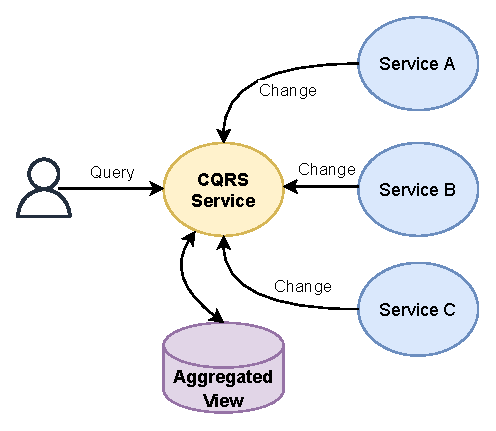
\includegraphics[scale=0.7]{images/Figure21}
		\end{center}
		\vspace{-0.6cm}
		\caption{CQRS pattern diagram.}
		\label{fig:fig21}
	\end{figure}

	\item \textbf{API composition}\label{par:composition} is a simple way to query data in a microservice architecture~\cite{richardson2018microservices, 8890660}, alternative and more lightweight solution than CQRS. 
	
	The main difference between CQRS is that this patterns does not have its own data storage. When a request comes in, it accesses every single microservice containing data, combines the results, and then returns the combined result to client. Making it easier to implement, because database does not need to be refreshed every time when some change occurs in the system. On the other hand, it may yield a slower response, depending on how many services we need to contact for the information, their availability, and time to merge and prepare data in memory. 

	Figure~\ref{fig:fig22} shows an example diagram for API Compossition pattern.

	\begin{figure}[H]
		\begin{center}
			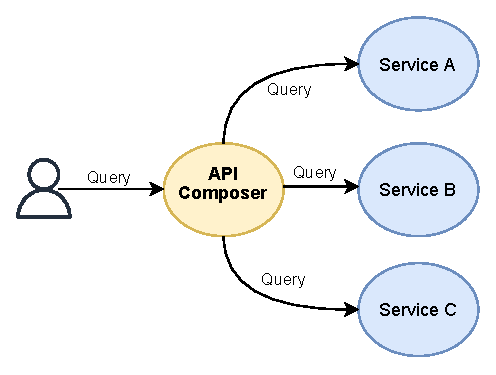
\includegraphics[scale=0.7]{images/Figure22}
		\end{center}
		\vspace{-0.6cm}
		\caption{API Compossition pattern diagram.}
		\label{fig:fig22}
	\end{figure}
\end{enumerate}

The best chance to succeed when implementing a microservices architecture is to simply follow existing patterns and use existing solutions with proven quality. 
%
%
\subsection{Observability}\label{sec:log_aggregation}
%
Observability is an integral part of any real-world computing system, and especially in the DS where observing what is happening in a network of processes is difficult~\cite{Fidge96}, due to the its nature.

In case of errors, fails or misbehavior of the system, some insight can be gained into what causes failure or which set of parameters in which circumstances. The three pillars of the observability are: \textbf{(1)} logs aggregation, \textbf{(2)} distributed tracing, and \textbf{(3)} alerting.

The logging operation, gives developers ability to store various arbitrary informations, that will provide more details for those who are investigating the failure. One thing we must be aware of is not to store any sensitive pieces of information in the log because this can cause a bunch of problems. Another thing we must be aware of is that we do not log too much and too often to slow down the business logic and execution of the function.

In monolithic applications logging and monitoring is a little bit easier to implement, because we have the whole application state in one place. When we come to the field of DS and microservices, our state is scattered across multiple elements or services. In DS, the monitoring involves interactions among concurrently executing processes~\cite{JoyceLSU87}.

The solution to this problem is to use a centralized logging service -- \textbf{logs aggregation}, that collects logs from each service~\cite{BeschastnikhWBE16}. This is beneficial because users can search and analyze the logs as a whole state of the system. To do this properly the log must be stored very reliably~\cite{DanielsST87}. Users can then configure the log server for some alerts that are triggered when certain messages appear in the logs. The log of DS usually does not contain enough information to regenerate the timeline of execution, and this is one reason that logs in DS are so hard to interpret~\cite{BeschastnikhWBE16}.

To resolve this problem of DS execution timeline, Google develops a new technique called \textbf{tracing}~\cite{36356}. The trace represents a single execution timeline or execution of one request. Trace will create a tree, and the tree is used to establish order. Every node in the tree represents a unit of work and it is called span. A tree unites all the elements needed to carry out an originating request. In every span or unit of work, we can attach more details about that particular execution element. 

Figure~\ref{fig:fig18} shows the simple example of \textit{RequestX} path through the processes in a distributed system, where each service \textbf{call} could be RPC, HTTP or some other request.

\begin{figure}[H]
	\begin{center}
		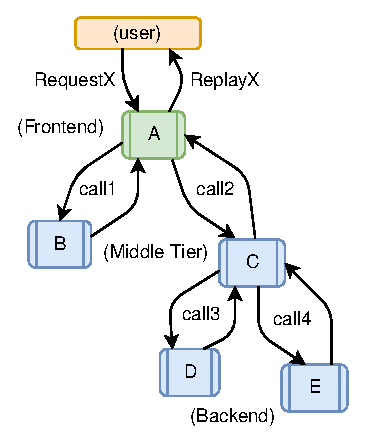
\includegraphics[scale=0.8]{images/Figure18}
	\end{center}
	\vspace{-0.9cm}
	\caption{\textit{RequestX} path through the processes in a distributed system.}
	\label{fig:fig18}
\end{figure}

\noindent
And last, but not the least option is \textbf{alerting}. Alerting of a monitored system can be represented as a set of rules that performs actions based on changes in specific metric. Alerting enables a system to notify users when something important happens or (probably) is going to happen.

DS logging, tracing and alerting represents the important role of any system, and as such, it should not be neglected especially in the DS environment. Every user request should be traced and logged from an infrastructure perspective, but we should allow users to store logs from their applications.
%
%
\section{Distribution Models}\label{sec:distribution_models}
%
The role of distribution models is to determine the responsibility for the request, or to answer the fundamental question \say{who is in charge} for a specific request. There are two ways to answer this question: \textbf{(1)} all nodes in the system, or \textbf{(2)} single node in the system.
%
%
\subsection{Peer-to-peer}\label{sec:p2p_networks}
%
Peer-to-peer (P2P) communication is a networking architecture model that partitions tasks or workloads between peers~\cite{Schollmeier01}. All peers are created equally in the system, and there is no such thing as a node that is more important than others. 

Every Peer has a portion of system resources, such as processing power, disk storage, or network bandwidth, directly available to other network participants, without the need for central coordination by servers or stable hosts~\cite{Schollmeier01}. P2P nodes are connected and share resources without going through a separate server computer that is responsible for routing. 

Figure~\ref{fig:fig2} shows difference in network topology between P2P networks $(left)$ and client-server architecture $(right)$.

\begin{figure}[H]
	\begin{center}
		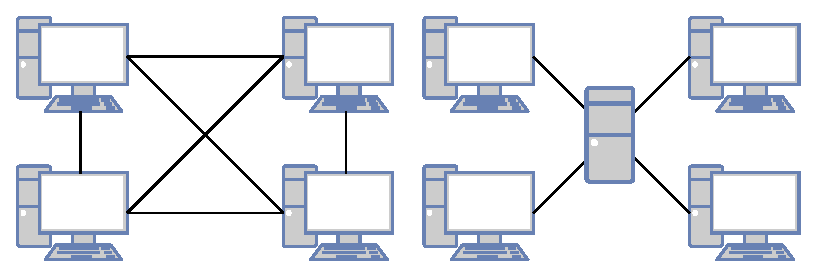
\includegraphics[scale=0.6]{images/Figure2}
	\end{center}
	\vspace{-0.6cm}
	\caption{P2P network and client-server network.}
	\label{fig:fig2}
\end{figure}

\noindent
Peers are creating a sense of virtual community. This community of peers can resolve greater tasks, beyond those that individual peers can do. Yet, these tasks are beneficial to all the peers in the system~\cite{BandaraJ13}. When a request comes to such a network, a node that accepts the request is usually called \textbf{coordinator}, because it then is trying to find the right peer to send a request to.

Based on how the nodes are linked to each other within the overlay network, and how resources are indexed and located, we can classify networks as~\cite{KamelSE07}:

\begin{itemize}
	\item \textbf{Unstructured} do not have a particular structure by design, but they are formed by nodes that randomly form connections~\cite{FilaliBHB11}. Their strength and weakness at the same time is the lack of structure. These networks are robust when peers join and leave the network. But when doing a query, they must find more possible peers that have the same piece of data. A typical example of this group is a Gossip-based protocol like~\cite{DasGM02}.
	\item \textbf{Structured} peers are organized into a specific topology, and the protocol ensures that any node can efficiently search the network for a resource. The famous type of structured P2P network is a Distributed Hash Table (DHT). These networks maintain lists of neighbors to do a more efficient lookup, and as such, they are not so robust when nodes join or leave the network. DHT is commonly used in resource lookup systems~\cite{StoicaMKKB01}, and as efficient resource lookup management and scheduling of applications, or as an integral part of distributed storage systems and NoSQL\cite{Leavitt10} databases.
	\item \textbf{Hybrid} combine the previous two models in various ways.
\end{itemize}

\noindent
P2P networks are a great tool in many arsenals, but because of their unique ability to act as a server and as a client at the same time, we must be careful and pay more attention to security because they are more vulnerable to exploits~\cite{0024003}.
%
%
\subsection{Master-slave}\label{sec:master_slave}
%
In the master-slave architecture, there is one node that is in charge -- \textbf{master}. This node accepts requests, and we usually do not communicate to the rest of the nodes or \textbf{slaves}. The master node is usually better and more expensive or even specialized hardware such as redundant array of inexpensive disks (RAID) to lower the crash probability. The cluster can also be configured with a \textbf{standby} master, and this node is continually updated from the master node.

But no matter how specialized hardware master runs on, it is prone to fail for various reasons, so it is a \textbf{single point of failure (SPOF)}. If crush happens, then standby master could continues to the server as a master, or new \textbf{leader election} protocol~\cite{KorachKM90} is initiated to pick a new master node. 

The master node is responsible for processing any updates to that data. If the master fails, then the slaves can still handle \textbf{read} requests. Failure of the standby master node to take over from the master node is a real problem if we want to achieve a high-availability system.

Figure~\ref{fig:fig16} shows difference between mater-slave $(left)$ and peer-to-peer $(right)$ request handling.

\begin{figure}[H]
	\begin{center}
		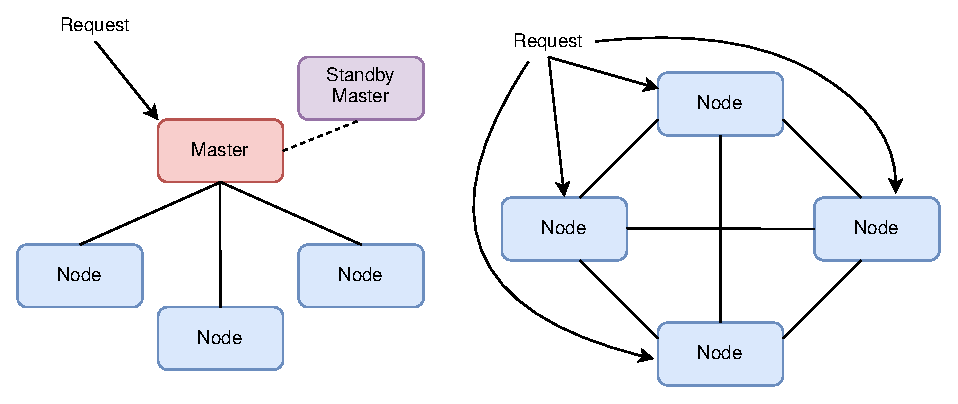
\includegraphics[scale=0.6]{images/Figure16}
	\end{center}
	\vspace{-0.6cm}
	\caption{Handling requests master-slave and peer-to-peer}
	\label{fig:fig16}
\end{figure}

\noindent
Using the right distribution model usually depends on the business requirements. High availability requires a P2P network because of no SPOF. If we could manage data using batch jobs that run in off-hours, then the simpler master-slave model might be the solution.
%
%
\section{Similar computing models}\label{sec:similar_models}
%
In this section, we are going to shortly describe models that are similar to the DS, and as such, they may be the source of confusion.
%
%
\subsection{Parallel computing}\label{sec:parallel_computing}
%
DC and parallel computing seem like models that are the same, and that may share some features like simultaneously executing a set of computations in parallel. Broadly speaking, this is not far from the truth~\cite{Vera16}. 

Differencies between the two can be presented as follows: in parallel computing, all processor units have access to the shared memory and have some way of the faster inter-process communication, while in DS and DC all processors have their memory on their machine and communicate over the network to other nodes which are significantly slower. 

These models are similar, but they are not identical, and the kinds of problems they are designed to work on are different. Figure~\ref{fig:fig4} visually summarizes the architectural  differences between DC $(up)$ and parallel computing $(down)$.

\begin{figure}[H]
	\begin{center}
		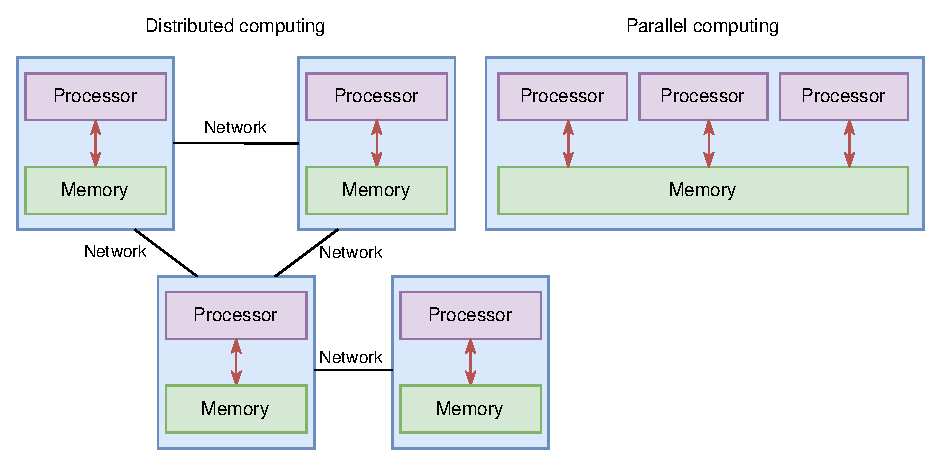
\includegraphics[scale=0.6]{images/Figure4}
	\end{center}
	\vspace{-0.6cm}
	\caption{Architectural difference between DC and parallel computing.}
	\label{fig:fig4}
\end{figure}

\noindent
Parallel computing has often used the strategy with problems that due to their nature or constraints must be done on multi-core machines simultaneously~\cite{0072397}. It is often that some big problems are divided into smaller ones, which can then be solved at the same time. 

Several tasks require parallel computing like simulations, computer graphics rendering, or different scenarios in scientific computing.
%
%
\subsection{Decentralized systems}\label{sec:decentralized_systems}
%
Decentralized systems are similar to DS, in a technical sense, they are still DS. But if we take a closer look, these systems \textbf{should not} be owned by a single entity. CC, for example, is a perfect example of DS, but it is not decentralized by its nature. It is a centralized system by the owner like AWS, Google, Microsoft, or some other private company because all computation needs to be moved to big DCs~\cite{HossainRH18}.

By modern standards, when we are talk about decentralized systems, we usually think of blockchain or blockchain-like technology~\cite{LeibleSSG19}, since here we have distributed nodes, that are scattered and there is no single entity that owns all these nodes. But even if this technology is run in the cloud, it is loses the decentralized feature. This is the caveat we need to be aware of. These systems are facing different issues because any participant in the system might be malicious and they need to handle this case. 

Nonetheless, CC can and should be decentralized in the sense that some computation can happen outside of cloud big DCs, closer to the sources of data. These computations could be owned by someone else, and big cloud companies could give their solution to this as well to relax centralization and problems that CC will have especially with ever-growing IoT and mobile devices.
%
%
\section{Transactions}\label{sec:transactions}
%
Transactions are keeping data consistent even in the presence of highly concurrent data accesses and despite all sorts of failures~\cite{WeikumV2002}. Transactions are trying to resolve this problem in a generic way, in such a way that is invisible to the application logic.

The main goal of transactions is to maintain system integrity in the consistent state, by ensuring that all operations on the system are either all completed successfully or all canceled successfully. Transactions are typically used in systems that needs to preserve some state (e.g. database or some filesystems). 

In their book Gray et al. make a good parallel with the contract law, saying that transactions give us the ability to \emph{clean up the situation}, if something does not work right.~\cite{GrayR93}.

Transactions guarantee following four properties: \textbf{(1)} atomicity, \textbf{(2)} consistency, \textbf{(3)} isolation, and \textbf{(4)} durability, also known as \emph{ACID} properties.
%
%
\subsection{Distributed transactions}\label{sec:distributed_transactions}
%
Because of the nature of DS, more network hosts are involved which significantly complicates the transaction mechanism. Distributed transactions are required to have all four \emph{ACID} properties. This might not be so easy to achieve amongst other due to \emph{CAP} theorem~\pageref{lab:cap}. 

In their book, Morgan et al. claim that here exists no distributed commit protocol that can guarantee independent process recovery in the presence of multiple failures (e.g., network partitionings)~\cite{WeikumV2002}.

Distributed transactions include few protocols such as two-phase commit (2PC), three-phase commit (3PC), Paxos, and various other approaches to quorum giving programmers facade of global serializability~\cite{Helland07}. 

Avoiding distributed transactions allows a much simpler, more robust and efficient solution.
%
%
\subsection{Sagas}\label{sec:sagas}
%
In 1987, Molina et al. presented \emph{Sagas}~\cite{Garcia-MolinaS87} and their work in the area of \emph{long-lived transactions (LLTs)}, types of transactions that hold resources for long periods, and as such delay shorter and more common transactions. 

These transactions are increasingly relevant and important, in the current technological landscape with the distribution of components and microservices architectures.

The saga transaction is composed of sub-transactions, executed in an atomic way so that either all or none of the sub-transactions take effect. However, no isolation is necessarily guaranteed between the sub-transactions of different sagas.

One transaction $T$ is composed of multiple sub-transactions $T_1,\ldots,T_n$, and every sub-transaction $T_i$ has an associated \emph{compensating transaction} $C_i$ or how the effects of the transaction can be rolled back. The saga transaction executes sub-transactions sequentially.

Figure~\ref{fig:fig20} shows an example of one transaction separated into multiple sub-transactions where \emph{green} arrows represent success path, while \emph{red} arrows represent rollbacks, structure of the saga transaction and at least the previous and next element in the chain.

\begin{figure}[H]
	\begin{center}
		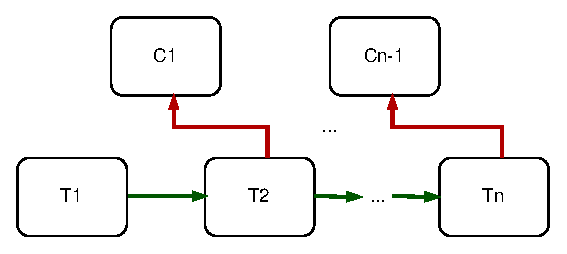
\includegraphics[scale=0.9]{images/Figure20}
	\end{center}
	\vspace{-0.6cm}
	\caption{Saga transactions separated in sub-transactions.}
	\label{fig:fig20}
\end{figure}

\noindent
Sagas can be implemented using two patterns: \textbf{(1)} orchestration where one centralized element is responsible for all the coordinating, or \textbf{(2)} choreography, where each service trigger local transactions in other services.

This isolation can be added in the application layer~\cite{Frank}l for example using \emph{semantic lock}. This strategy will change state so that some data are in process and should be treated differently. 

For example, an order can be in one of the following states: \textbf{(1)} \emph{PENDING}, \textbf{(2)} \emph{COMPLETED}, or \textbf{(3)} \emph{CANCELED} state. Other transactions will not make use the data if status is not set to \emph{COMPLETED}.
%
%
\section{Garbage collection}\label{sec:garbage_collection}
%
Most modern programming languages nowadays allow programmers to allocate and free memory. This process can be in total responsibility of the programmer, or language can handle this process for the programmer. When there is some automatic process involved to release unused resources, that process is called \textbf{garbage colection} or GC. 

In~\cite{JonesL96}, Jones, et al. describe \emph{garbage collection} as the automatic management of dynamically allocated storage. However, the term \emph{garbage collection} is not exclusive to programming languages. It is widely used to refer to all forms of automatic management of dynamically allocated resources.

Even with the rapid growth of memory sizes, and lowering the overall cost of memory is not inexhaustible. Like any other limited resources, it requires careful consideration and recycling. Even tools like Kubernetes, have some form of garbage collection that is used to remove unused items and their references in the system.

Over the years, different algorithms are used to do reference counting and tracing methods, to discover unused resources, and to free them. One of the most common algorithms for garbage collection is \emph{mark-sweep} algorithm~\cite{McCarthy60} developed in 1960. The variety on the topic exists today, but the essence of the algorithm remains widely used today.

Traditional automated garbage collection is usually seen as slow, and disruptive to executing programs. Modern implementations of the garbage collection substantially reduced the overhead of the system~\cite{JonesL96}.
%
%
\section{Virtualization techniques}\label{sec:virtualization_techniques}
%
Virtualization as a technique started long ago in time-sharing systems, to provide isolation between multiple users sharing a single system like a mainframe computer~\cite{CrosbyB06}. 

In~\cite{Sharma} Sharma et al. virtualization is described as technologies that provide a layer of abstraction of the physical computing resources between computer hardware systems and the software systems running on them.

Modern virtualization differentiates several different tools. Some of them are used as an integral part of the infrastructure for some flavors like IaaS, while others are used in different CC flavors as well as microservices packaging and distribution format, or are new and still are looking for their place. These options are:

\begin{itemize}
	\item \textbf{Virtual machines (VM)} are the oldest technology of the three. They are described as a self-contained operating environment consisting of guest operating system and associated applications, but independent of the host operating system~\cite{Sharma}. VMs enable us to pack isolation and better utilization of hardware in big DCs. They are widely used in IaaS environment~\cite{AbsalomBJ13, YangHCLW13} as a base where users can install their own operating system (OS) and require software tools and applications.
	\item \textbf{Containers} provide the almost same functionality to VMs, but there are several subtle differences that make them a go-to tool in modern development. Instead of the guest OS running on top of host OS, containers use tools that are in a Linux kernel like \textit{cgroups} that limit process resource usage so that single process can not starve other processes and use all the resources for itself, and \textit{namespaces} to provide isolation and partitions kernel resources so that single process sees node resources like it only exists there. Containers reduce time and footprint from development to testing to production, and they utilize even more hardware resources compared to VMs and show better performance compared to the VMs~\cite{Seo2014PerformanceCA, FelterFRR15}. Containers provide an easier way to pack services and deploy and they are especially used in microservices architecture and service orchestration tools like Kubernetes~\cite{BurnsGOBW16}. Google has stated several times in their online talks that they have used container technology for all their services, they even run VMs inside containers for their cloud platform. Even though they exist for a while, containers get popularized when companies like Docker and CoreOS developed user-friendly APIs.
	\item \textbf{Unikernels} is the newest addition to the virtualization space. Unikernels are defined as small, fast, secure virtual machines that lack operating systems~\cite{pavlicek2016unikernels}. Unikernels are comprised of source code, along with only the required system calls and drivers. Because of their specific design, they have a single process and they contain and execute what it absolutely needs to nothing more and nothing less~\cite{GoethalsSAVT18}. They are advertised as new technology that will save resources and that they are \textit{green}~\cite{208735}, meaning they save both power and money. When put to the test and compared to containers they give interesting results~\cite{GoethalsSAVT18, PlauthFP17}. Unikernels are still a new technology and they are not widely adopted yet. But they give promising features for the future, especially \textbf{if} properly ported to ARM architectures, and various development languages. Unikernels will probably be used as a user application and function virtualization tool, because of their specific architecture, especially for serverless applications presented in~\ref{sec:microservices}.
\end{itemize}

\noindent
With every virtualization technique, the ultimate goal is to pack as many applications on existing hardware as possible, so that there are no resources that are left not used -- we are trying to achieve high resource utilization. 

Figure~\ref{fig:fig5} represents architectural differences between VMs, containers, and unikernels.

\begin{figure}[H]
	\begin{center}
		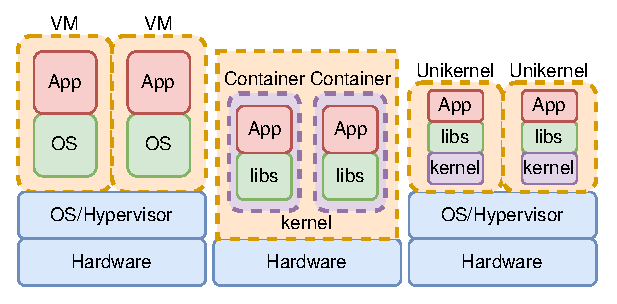
\includegraphics[width=\linewidth]{images/Figure5}
	\end{center}
	\vspace{-0.6cm}
	\caption{Architectural differences between VMs, containers and unikernels.}
	\label{fig:fig5}
\end{figure}
%
%
\section{Deployment}\label{sec:deployment}
%
Over the years different approaches evolved how to deploy infrastructure and applications. The difference just gets more amplified, when CC and microservices get into the picture, where frequent deployment is very common. 

Deployments in such complex environment can be separated by how they handle changes on existing infrastructure or applications on:

\begin{itemize}
	\item \textbf{A mutable model} is a model where we have in place changes which mean that the parts of the existing infrastructure or applications get updated or changed to do an update. In place change can produce some problems, and has:
	
	\begin{enumerate}[start=1,label={(\bfseries \arabic*)}]
		\item more risk because in-place change may not finish, which puts our infrastructure or the application in a possible bad state. This is especially a problem if we have a lot of services and multiple copies of the same service. The possibility that our system is not on is a lot higher.
		\item high complexity, this is a direct implication of the previous feature. Since our change might not get fully done, it cannot be guaranteed that our infrastructure or application is transitioned from one version to another -- change is not \textbf{discrete}, but \textbf{continues} since we might end up in some state in between where we are now and where we want to be.
	\end{enumerate}
	
	\item \textbf{An immutable model} is a model where no in-place changes on existing infrastructure or application are done whatsoever. In this model, the previous version is replaced completely with a new version that is updated or changed compared to the previous version. The previous version gets discarded in favor of the new version. Compared to the previous model, immutable deployment:
	
	\begin{enumerate}[start=1,label={(\bfseries \arabic*)}]
		\item has less risk, since the existing infrastructure or the application, is not changed, but a new one is started and the previous one is shut down. This is important especially in DS where everything can fail at any time.
		\item has less complexity of the mutable deployment model. This is a direct implication of the previous feature since the previous version is shut down and fully replaced with the new one. This is a \textbf{discrete} version change and atomic deployment with deferring deployments with fast rollback and recovery processes.
		\item requires more resources~\cite{Helland16}, since both versions must be present on the node for this process to be done. The second problem is the data that the application has generated should not be lost. The problem is solved by externalizing the data. We should not rely on local storage but store that data elsewhere, especially when the parts of the system are volatile and changed often. The key advantage of this approach is avoiding downtime experienced by the end-user when new features are released. 
	\end{enumerate}
\end{itemize}

Immutability is a simple concept to understand and simplifies a lot especially in DS~\cite{Helland16}. Write down some data, and ensure that it never changes. It can never be modified, updated, or deleted~\cite{perry2020art}. When this is combined with the promise that downtime can be avoided especially in complex DS, it is clear why the immutable model is gaining more and more popularity (especially with the arrival of containers). 

Immutable infrastructure deployment offers several benefits on how to deploy changes. Even in production, it is easier to switch to a whole new version. These strategies include:

\begin{itemize}
	\item \textbf{Blue-Green deployment}, this strategy requires two separate environments: \textbf{(1)} \textit{Blue} current running version, and \textbf{(2)} \textit{Green} is the new version that needs to be deployed. When there is satisfaction that the green version is working properly, the traffic can be gradually rerouted from the old environment to the new one,  for example by modifying the Domain Name System (DNS). This strategy offers near-zero downtime.
	\item \textbf{A canary update} is a strategy where a small subset of requests is directed to the new version --- the canary, and the rest of them are directed to an old version. If the change is satisfactory, the number of requests can be increased, and it should be monitored how the service is working with increasing load, if there are errors, etc.
	\item \textbf{Rolling update} strategy updates large environments, a few nodes at the time. The setup is similar to blue-green deployment, but here there is a single environment. With this strategy, the new version gradually replaces the old one. If for whatever reason the new version is not working properly on the larger number of nodes, rolling back to the previous version can always be done.
\end{itemize}

\noindent
With mutable infrastructure, these strategies would be hard to implement, and maybe it is not possible at all. Besides infrastructure deployment, there is another side that we must be considered, and that is how to describe these deployments. Two different strategies can be considered here:

\begin{itemize}\label{lab:dep_types}
	\item \textbf{Imperatively}, with this option users have to write code or specific instructions step by step what the specific tool needs to do so that the application or infrastructure is properly set up. In this approach, we have a \textit{smart} user who describes \textit{dumb} machine what is needed to be done and in what order to achieve the desired state.
	\item \textbf{Declaratively}, with this option a user has to describe the end state or what is his desired state, and the tool needs to figure out the way how to do this. Here we have a \textit{smart system} that will find a way how to achieve the \textbf{desired state}, and we have a user who\textit{does not care} in what order actions need to be done --- that is what the system needs to do. Users do not need to worry about timing, this simplifies the whole process and the code always represents the latest state. With this type of deployment, we can offer users, two different models:
	
	\begin{enumerate}[start=1,label={(\bfseries \arabic*)}]
		\item using existing platform independent formats that users are familiar with, like \textit{JSON, YAML, XML}, etc.
		\item using a domain-specific language (DSL) that users need to learn, but we might be able to optimize description.
	\end{enumerate}
\end{itemize}

\noindent
So far, the first option is preferred by many companies, because users are already familiar with these formats, and does not require developers time to develop new DSL. If the platform becomes too complicated then it makes sense to develop DSL for this purpose.

Figure~\ref{fig:fig12} summarizes the difference between mutable and immutable deployment models.

\begin{figure}[H]
	\begin{center}
		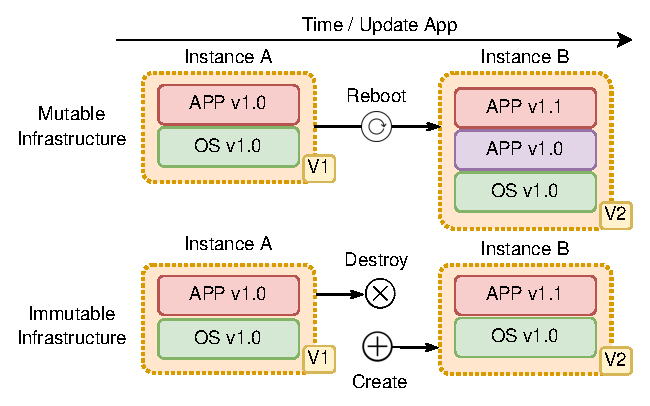
\includegraphics{images/Figure12}
	\end{center}
	\vspace{-0.6cm}
	\caption{Difference between mutable and immutable deployment models.}
	\label{fig:fig12}
\end{figure}

\noindent
With the introduction of \textit{LinuxKit}, Linux subsystems are based around very secure containers. With LinuxKit, every part of the Linux subsystem runs inside the container, so a Linux subsystem can be assembled with services that are needed. As a result, systems created with LinuxKit have a smaller attack surface~\cite{abs-1802-10375} than general-purpose systems. 

This is important not only from the security point of view but also for infrastructure deployment as well. Specific OSs can be created, based on the containers for a different purpose. They can be updated, changed, and adapted for every machine or purpose needed.

Deployment is based on changing parts of the OS, and services that run inside the containers. As a result, everything can be removed or replaced. It's highly portable and can work on desktops, servers, IoT, mainframes, bare metal, $\upmu$DCs at the edge, and virtualized systems.

\section{Infrastructure as software}~\label{sec:ias}
%
The infrastructure needs to be constantly deployed and maintained, so it would be beneficial to view the infrastructure as software (IaS)~\cite{Fitzgerald}. The benefit of this approach lies in the already available tools, principles, and techniques (e.g. reuse, testing, modeling, and evaluation) that can equally be used for the infrastructure definitions ~\cite{Osterweil, Fitzgerald}.

In his work~\cite{Osterweil}, Osterweil et al. argue that software and software processes share some similar characteristics: \textbf{(1)} both are executed, \textbf{(2)} both have requirements that need to be understood, \textbf{(3)} both benefit from being modeled, and \textbf{(4)} both can be guided by measurement.

Fitzgerald et al.~\cite{Fitzgerald} argue that process programming, defined by Osterweil~\cite{Osterweil} et al., is applicable in the infrastructure domain. The authors claim that it is useful to extend the “software process as software” paradigm to include infrastructure as software (IaS). The move towards multi-tier systems that involve cloud and cyber-physical systems will only stimulate the connection between software and reliable infrastructure systems.

Looking at the infrastructure configuration as the software allows application developers to venture into the “infrastructure programming”~\cite{Fitzgerald}, allowing platforms and infrastructure to be managed in a similar way as the software is.

In a cloud environment, it is an essential technique to properly implement continuous deployment, giving us tools to automate the configuration and provisioning process of infrastructure using cloud instances~\cite{RahmanMW19}. Wittig et al. describe it as a process of managing and provisioning computer data centers through machine-readable definition files, rather than physical hardware configuration or interactive configuration tools~\cite{wittig2018amazon}. 
%
%
\subsection{Infrastructure as code}
%
In modern cloud and microservices era, a new strategy to manage and deploy complicated infrastructure elements -- Infrastructure as code (IaC). In his book~\cite{wittig2018amazon} Wittig et al. describe it as a process of managing and provisioning computer data centers through machine-readable definition files, rather than physical hardware configuration or interactive configuration tools. 

IaC has grown in popularity in recent years because it applies the same kind of version control and repeatability to the orchestration of the infrastructure as developers use for applications source code~\cite{ArtacBNGT17}. The second benefit is that configuration is decoupled from the system, it can more readily be deployed on a similar system elsewhere. 

IaC is a continuation of earlier works of Osterweil et al.~\cite{Osterweil}, and Fitzgerald et al.~\cite{Fitzgerald}, trying to move infrastructure to level of software, keeping existing tools, best practices and techniques. It relys on the \textbf{reconciler pattern}~\cite{luksa2018kubernetes}, widely used in scheduling systems like Kubernetes.

This pattern enables tracking of resources using two simple states: \textbf{(1)} expected state, and \textbf{(2)} current state. The expected state represents the desired state, while the current state refers to the actual system state. The reconciler pattern runs a \textbf{reconciliation loop} that ensures that the current state remains the same as the expected state.

Every node must provide its current state regularly, and when some state is divergent from the desired state, the system must act to ensure that this situation is corrected automatically. The node can send its state over existing channels e.g., \textbf{health-check} pings to minimize load and data transferred over the network, or a dedicated channel just for this purpose may exist.
%
%
\section{Development roles}\label{sec:dev_roles}
%
In our modern internet-connected world of applications, we have several distinctive development roles. Each of them plays an important role so that modern software runs smoothly, and with less downtime. These development roles could be separated into a few categories (focus is on the technical roles):

\begin{itemize}
	\item \textbf{A developer} is usually a person responsible for developing software for the user. A developer is responsible for maintaining existing, and/or developing new features. There could be different sub-roles, dealing with specific parts of the complex software systems.
	\item \textbf{DevOps} role represents a multidisciplinary organizational effort to automate application deployments through continuous delivery of new software updates~\cite{LeiteRKMM20}. It combines software development with technology operations~\cite{JabbariAPT16} to shorten the development life cycle.
	\item \textbf{Site Reliability Engineer (SRE)} role is responsible for availability, latency, performance, efficiency, change management, monitoring, emergency response, and capacity planning~\cite{beyer2016site}. It is a software engineering role and needs to have an understanding of the fundamentals of computing~\cite{JonesUN15}, applied to the infrastructure and operations problems.
\end{itemize}

\noindent
DevOps and SREs seem to be similar roles, they are both trying to bridge the gap between development and operations. As such they have a very large conceptual overlap in how they operate~\cite{46939}, but also have some differences. 

Table~\ref{tab:table10} sums the differences between the DevOps and SREs.

\begin{table}[H]
	\begin{center}
		\begin{tabular}{l|l|l}
			\textbf{Feature} & \textbf{DevOps} & \textbf{SREs}\\
			\hline
			\textbf{Task} & \multirow{2}{10em}{Scaling, uptime, robustness} & \multirow{2}{10em}{Development pipeline} \\
			& & \\
			\textbf{Essence} & Practices and metrics &  Mindset and culture \\
			\textbf{Team structure} & \multirow{3}{10em}{Wide range of roles: QA, developers, SREs etc.} &  \multirow{3}{10em}{SREs with operations and development skills} \\
			&  &  \\
			&  &  \\
			\textbf{Focus} & \multirow{2}{10em}{Development and delivery continuity} & \multirow{2}{10em}{System availability and reliability} \\
			&  &  \\
			\hline
			\textbf{Goal} & \multicolumn{2}{c}{\multirow{2}{15em}{Bridge the gap between development and operation}} \\
			&  &  \\
		\end{tabular}
	\end{center}
	\vspace{-0.5cm}
	\caption{Differences between DevOps and SREs.}
	\label{tab:table10}
\end{table}

\noindent
In modern complex software development, SREs should keep things running smoothly, while DevOps principles should be used to improve processes. 

So it is not either/or, but it seems that a combination of approaches may provide the best results. However, in some smaller organizations, these roles can overlap.
%
%
\section{Concurrency and parallelism}\label{sec:concurency_parallelism}
%
People usually confuse these two concepts. Even though look similar, they are a different way of doing things. In his speech, Rob Pike~\cite{Pike} gives a great explanation and examples on this topic. He also gives great definitions of these concepts like:

\begin{itemize}
	\item \textbf{Concurrency} is composition of independently executing things. Concurrency is about dealing with a lot of things at once.
	\item \textbf{Parallelism} is the simultaneous execution of multiple things. Parallelism is about doing a lot of things at once. 
\end{itemize}

\noindent
These things are important, especially when building applications and systems that should achieve very high throughput. They must be built with a good structure and a good concurrence model. These features enable possible parallelism, but with communication~\cite{Pike}. These ideas are based on Tony Hoare work of Communicating Sequential Processes (CSP)~\cite{Hoare78}.

\subsection{Actor model}\label{sec:actor_model}
%
An actor model, the main idea is based around \textbf{actors} which are small concurrent code, that communicate independently by sending messages, removing the need for lock-based synchronization~\cite{Hewitt}. This model proposes a similar idea to Tony Hoare's in his work with CSP~\cite{Hoare78}, and actors are often confused with CSP. 

Table~\ref{tab:table6} gives differences between an actor model and CSP.

\begin{table}[h!]
	\begin{center}
		\begin{tabular}{l|l|l}
			\textbf{Feature} & \textbf{CSP} & \textbf{Actor model}\\
			\hline
			\textbf{Fault tolerance} & Distributed Queue &  Supervisors hierarchy \\
			\textbf{Process identity} & Anonymus & Concrete \\
			\textbf{Composition} & NA & Applicable \\
			\textbf{Communication} & Queue & Direct \\
			\textbf{Message passing} & Sync & Async\\
		\end{tabular}
	\end{center}
	\vspace{-0.5cm}
	\caption{Differences between actor model and CSP.}
	\label{tab:table6}
\end{table}

\noindent
Actors do not share a memory, and they are isolated by nature. An actor can create another actor/s and even watch on them in case they stop unexpectedly. When an actor finished its job, and it is not needed anymore, it disappears. These actors can create complicated networks that are easy to understand, model, and reason about, and everything is based on a simple message passing mechanism. 

Every actor has a designated message box. When a message arrives, the actor will test the message type and do the job according to the message type he received. In this way, we are not dependent on lock-based synchronization that can be hard to understand, and it can cause serious problems.

The actor model is fault-tolerant by design. It supports crush to happen because there is a \say{self-heal} mechanism that will monitor actor/s, and when the crash happens it will try to apply some strategy, in most cases just restart actor, but other strategies could be applied. This philosophy is useful because it is hard to think about every single failure option.
%
%
%!TEX root =  main.tex
\chapter{Research review}\label{chapter:Review}
%
%
%



\section{Platform models}\label{sec:platform_models}
%
%



\section{Nodes organization}\label{sec:nodes_organization}
%
%


\section{Task offloading}\label{sec:task_offloading}
%
%



%!TEX root =  main.tex
\chapter{Micro clouds and edge computing as a service}\label{chapter:Micro_clouds}
%
This section explains the model of EC as a service compared to the traditional CC model. We present the formation of such a system with a formal model and proof of concept implementation based on the proposed model.

In Section~\ref{sec:configurable_model_structure} present configurable model used to describe our system. in Section~\ref{sec:separation_of_concerns} we present separation of concerns for our model. In Section~\ref{sec:as_a_service_model} we discuss how this system could be offered as a service model and could be used for EC as a service. In Section~\ref{sec:application_model} we present possible application model and how users can utilize newly created architecture fully, using existing application models. Section~\ref{sec:immutable_infrastructure} present desired option for infrastructure deployment. In Section~\ref{sec:formal_model} we present why formal models are important in computer science and DS in particular, as well as model of our system with all protocols and nodes properties. Section~\ref{sec:repercussion} give repercussion of proposed model, and how it can be used as stand alone model where other features could be implemented on top of that or used as service for other, existing, systems. Finally, section~\ref{sec:limitations} present limitation of our model.
%
%
\section{Configurable Model Structure}\label{sec:configurable_model_structure}
%
Satyanarayanan et al.~\cite{SatyanarayananK19} propse architecture eparated into 3 tiers. Combained with MDCs and a zone-based server organization we get a good starting point for building EC as a service and micro cloud system, because we can extend the computing power and storage capacity serving local population. But, we need a more available and resilient system with less latency. To do that we need to extend these concepts and adopt them for different usage scenario.

If we take a look at the CC design, every part contributes to a more resilient and scalable system. Regions (or DCs) are isolated and independent from each other, and also contain resources application needs. They are usually composed of few availability zones~\cite{SouzaMFAK19}. If the one zone fails, there are still more of them to serve user requests. With some adaptations, EC could use a similar proven strategy. That strategy could be than used in applications beyound just EC.

Table~\ref{tab:table5} shows similar concepts between CC and edge centric computing (ECC) concepts, with accent on difference what is the physical part, and what are logical concepts.

\begin{table}[h!]
	\begin{center}
		\begin{tabular}{l|l}
			\textbf{Edge centric computing} & \textbf{Cloud computing}\\
			\hline
			Topology (logical) & Cloud provider (logical)\\
			Region (logical) & Region (physical)\\
			Cluster (physical) & Zone (physical)\\
		\end{tabular}
	\end{center}
	\vspace{-0.5cm}
	\caption{Similar concepts between cloud computing and ECC.}
	\label{tab:table5}
\end{table}

We can combine multiple node clusters into a bigger logical concept of $region$, increasing availability and reliability of both system and applications. We are talking about geo-distributed systems, so we have a bit of a different scenario than in the standard CC model. The cloud region is a physical thing~\cite{SouzaMFAK19}, while in the ECC a region could be represented in a different way. We now give a forma definition of a $region$ in ECC as:

\begin{definition}
	In geo-distributed ECC and micro clouds, a regoin is used to describe a set of clusters over an arbitrary geographic region. 
\end{definition}

Regions can accept or release clusters and clusters can accept or release nodes. Based on this property, we can define minimum size of an ECC region as:

\begin{definition}
	ECC regions are composed of at least one cluster, but can be composed of much more, so as to achieve a more resilient, scalable, and available system. 
\end{definition}

To ensure less latency in the system, vast distance between clusters should be avoided in normal circumstances. In a CC, region extension requires physically connecting modules to the rest of the infrastructure \cite{Hamilton07}.\\ 

Multiple regions form a second logical layer - $topology$. Formaly, we can define a $topology$ in ECC as:

\begin{definition}
In geo-distributed ECC and micro clouds, topology is a logical concept composed of a minimum one region, and could span over more regions. 
\end{definition}

When designing a topology, especially if regions need to share information, vast distance between regions should be avoided, if possible. With these simple abstractions, we can cover any geographic region with the ability to shrink or expand clusters, regions, and topology. Separation on $clusters$, $regions$, and $topologies$ is a matter of agreement and usages similar to modeling in Big Data systems~\cite{SonbolOAA20, WangCAL14}. 

For example, clusters could be as wide as the whole city or small as all devices in a single household and everything in between. The city could be one region with parts of the city being organized into clusters. We can form a city topology by splitting the city into multiple regions containing multiple clusters, or we can form a country topology by splitting the country into regions, with cities being regions. We can follow a more natural administrative division of some region, and organize resources by population usages.

Nodes inside the cluster should run some membership protocol. Gossip style protocols, like SWIM~\cite{DasGM02}, could be used in conjunction with replication mechanisms~\cite{LiBCL20, CauCBFCEB16,CRDTS_Nuno} making the whole system more resilient. In~\cite{inproceedingsSimic2} Simi\' c et al. take a look from theoretical point of view on conflict free replicated data types (CRDTs) usage, to achieve SEC in EC and conclude that CRDTs could be natural fit to EC as long as we are aware of potential pitfals of CDRTs.

Single $topology$ reflects one CC provider, so multiple $topologies$ are forming $micro-clouds$ that are able to help CC with huge latency issues, pre-processing in huge volumes of data and relax and decentralize strict centralized CC model.

These micro-clouds have much less resources, copared to standard clouds but they are much closter to the user meaning they have much fater response. In case of storage, if data is not present in the time of user request, they can pull data from the cloud and cache it for latter.

This 3 thier acrchitecture with numerous clients in the bottom, micro clouds in the middle, and cloud on the top kinda resembles cache level architecture in CPU~\cite{FarshinRMK19}. On lower levels we have fastest response time, since data is on the device. But at the same time, we have very limited storage capacity and processing power. As we go on upper tiers, we have more and more storage capacity and processing power, but contrary the response time is higher and higher.  Esspecially when we take distance into consideration, and huge volumes of data that need to be moved to the cloud.

Figure~\ref{fig:fig9}. shows the 3 tier architecture, with the response time and resource avelability.

\begin{figure}[H]
	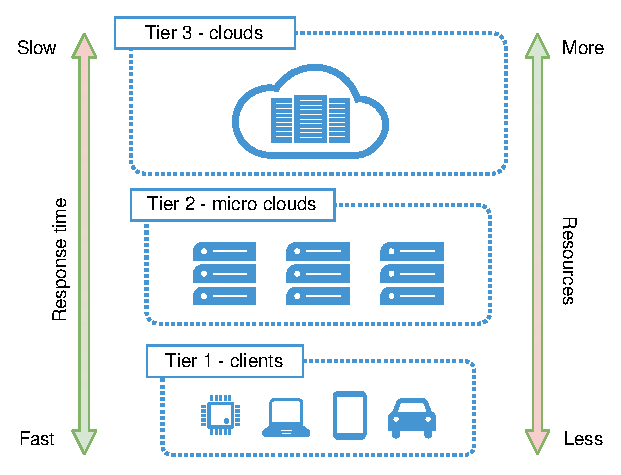
\includegraphics[width=\linewidth]{images/Figure9}
	\vspace{-0.7cm}
	\caption{3 tier architecture, with the response time and resource avelability}
	\label{fig:fig9}
\end{figure}

In everything as a service model~\cite{DuanFZSNH15}, EC as a service fits in between CaaS and PaaS, depending on users needs. 
%
%
\section{Separation of concers}\label{sec:separation_of_concerns}
%
To describe physical services, Jin et al.~\cite{JinCJL14} proposes three core concepts and specifies their relationships. These concepts are: $(1)$ Devices, $(2)$ Resources, and $(3)$ Services. 

SoC is a vital part of any system, especially if creating a platform to offer as a service. We based our SoC model for ECC as a service on these concepts, with adaptations for our use case, separated in three layers depicted in Figure~\ref{fig:fig10}. 

The bottom layer consists of various devices, or data creators and services consumers. The second layer represents resources. Resources have a spatial feature and indicate the range of their hosting devices~\cite{JinCJL14}. Developers at any time must know the resource utilization and spread, as well as application's state and health. 

Resources represent EC nodes, and to be part of the system, a node must satisfy four simple rules:

\begin{enumerate}[start=1,label={(\bfseries \arabic*)}]
\item run an operating system with a file system 
\item be able to run some application isolation engine, for example a container or unikernels 
\item have available resources for utilization 
\item have stable internet connection
\end{enumerate}

Services expose resources through an interface and make them available on the Internet~\cite{JinCJL14}. These services respond to clients immediately if possible, or cache information~\cite{SatyanarayananBCD09,YaoXWYZP20} for future requests. Services in the cloud should be able to accept pre-processed data, and they are responsible for computation and storage that is beyond the capabilities of ECC nodes. Services in the cloud should be able to take direct requests from client just in case that something catastrific happend to the micro-cloud that is close to the user.

Figure~\ref{fig:fig10}. shows the proposed SoC for every layer of the ECC as a service model.

\begin{figure}[H]
	\includegraphics[width=\linewidth]{images/FIG1}
	\vspace{-0.7cm}
	\caption{ECC as a service architecture with separation of concerns.}
	\label{fig:fig10}
\end{figure}
%
%
\section{As a service model}\label{sec:as_a_service_model}
%
Users should be able to develop their applications using two different models:
 
\begin{enumerate}[start=1,label={(\bfseries \arabic*)}]
	\item \textbf{microPaaS or mPaaS}, where the platform is doing all the management and offers a simple interface for developers to deploy their applications. This model is similar to PaaS, and the only difference is that this is running in micro-cloud and synchronize with CC.
	\item \textbf{microCaaS or mCaaS}, if users require more control over resources requirements, deployment and orchestration decisions. This model is similar to CaaS, and the only difference is that this is running in micro-cloud and synchronize with CC.
\end{enumerate}

Both variants should not stand alone, at least not for now. Fot that same reason we do not have microSaaS or mSaaS option, since that woul requre that whole application is running \textbf{only} in micro-clouds. But both options could be included, and part of any cloud model presented in~\ref{sec:cloud_computing}, or offered separatly.
%
%
\section{Applications Model}\label{sec:application_model}
%
Traditional DCs and CC propose specially designed cloud-native applications~\cite{GannonBS17}, that are easier to scale, more available, and less error-prone when compared to traditional web applications~\cite{GannonBS17}. Edge-native applications~\cite{SatyanarayananK19} should use the full potential of EC infrastructure, and keep good features of their cloud counterparts. 

Applications may be split in front and back processing services. Front processing service is an edge-native application running inside micro cloud to minimize latency, while the back service runs in traditional cloid as a cloud-native application to leverage greater resources. 

These edge-native applications will handle user requests coming to nearby MDCs, and communicate to cloud-native applications when needed. Separation like that gives developers better flexibility and large design space. 

Frontend services model should be event-driven, with a subscription policy to message streams using topics~\cite{inproceedingsBeck}. The processing strategy is in the developer's hands, depending on the nature of the use-case. 

Some examples may include:

\begin{enumerate}[start=1,label={(\bfseries \arabic*)}]
	\item \textbf{events} that notify users if some value is above or below some defined threshold 
	\item \textbf{stream} or processing data as it comes to the system 
	\item \textbf{batch} does processing in predefined times over some bigger collection of data 
	\item \textbf{other}, something that falls outside these models, or it is composition of multiple operations at once. This type should get events from some topic as they arrive, and user can define his own strategy what it needs to be done and how it needs to be pcessed. Usec can contact other existing services, and user is responsabile for optimization.
\end{enumerate}

These types of applications could be implemented in may ways like those disccused in~\ref{sec:microservices}, or some adapted variant of those models.

Section~\ref{sec:packaging} argue about how applications could be packed and deployed in the wild.
%
\subsection{Packaging}\label{sec:packaging}
%
Because their nature, micro clouds could be most likley composed of ARM devices. These devices in many cases are not able to run full VMs because their hardware restrictions. In recent years there are advances in VMs technology and their ability to run VMs on ARM devices. In~\cite{Ding12armvisor} Ding et al. show such possibility to run VMs on ARM devices.

But even if VMs are fully compatable with ARM devices, we still inherite VMs large footprint, already descused in~\ref{sec:virtualization_techniques} if we try to use tham $as is$.

On contrary, containers and unikernels give us $more for less$ same functionality but using less resources, meaning we can run more services in containers and even more in unikernels. But untill unikernels are fulkly ready to be used they will fall in nice to have category, and we should stick to containers. But even with containers we need to be aware of their limitations and pitfalls, and know that there is no $silver bullit$ and there is no one solution for all scenarios.

At the moment, containers are more matured solution than unikernels, and require less resources than VMs. On top of that, there are numerous of tools already existing using containers that could be utilized. Knowing all this, at first stages of micro-clouds, containres should be option to go. 

In~\cite{inproceedingsSimic3} Simi\' c et al. show benefits of using containres in large sclae edge computing systems from theoretical point of vew, by looking into architecture difference. Authors focus on differences between VMS and containers in cases where services needs to be runned on ARM devices with limited resources.

In future and when unikernels are more matured and tested, they could be used for paritical use-cases and applications, esspecially like events or serverless implementations. Containres will probably not be fully replaced, but they can co-exist with unikernels in some cases where we need more controll over running single function.

Like any other system, users can create their own variants of the systems and different flavours optimized for certen solutions. In that cases, they may favorized one solution over the other one. But in general case containers and unikernels should be prefered way to package, run and distributed user applicatoins in micro-clouds environment.
%
%

\section{Immutable infrastructure}\label{sec:immutable_infrastructure}
%
As described in~\ref{sec:deployment}, we have few options when it comes to setup and deply infrastructure and/or applications. This thesis propose DS model that is build with three tier architecture that should operate in geo-distributed environment we blieve that \textbf{immutable deployment} model would be good fit. It will simplify deployment process, since we want to rely on atomic operations and do not want to left misconfigured system at any level. If something like that happend, we will end up in problem, that would be hard to properly address and resolve.

Geo-distributed micro-clouds model that is described in this chaper, should operate in two levels of deployment that are build one on top of the another:

\begin{enumerate}[start=1,label={(\bfseries \arabic*)}]
	\item \textbf{Infrastructure deployement}, update and change should be atomic and immutable. Users should do changes declaratively --- mutations of the system, by telling the system what new state should be, and let the system to figure out the best way how to do user specified changes. In this category, we can account any change that is doing on the cluster, region or topology that user/s operate on. For example create of new cluster, region, topology or doing configurations of the setup system. The only change that could possible be done by imperative strategy is updates on the nodes itself. But even for this strategy, it would be beneficial if we could usedeclarative way \textbf{if possible}. It is important to notice that \textbf{mutation} does not mean in place change, but just name of operation. This deployment strategy is reserved for operations people, but if compay or team is small any developer could do this. Developers should not be dealing with this part of the deployment.
	\item \textbf{Services deployment}, make sense only if previous action is takane. We must have infrastructure setup already, in order do put any sort of services (applications) into the system. As previous model, this should be done declaratively as well, and all changes dould be done immutably without any in place change. User should specify his new state or \say{view of the word} declaratively and let system do all the changes he wants. All user services should be packed as described in~\ref{sec:packaging} because this simplifies way services are put to the nodes. When done properly, this allow operations people to do faster changes with almost zero downtime deployments with all strategies already discused in~\ref{sec:deployment}. this part of the deployemnt should be done by developers, since they done implementation and testing. They know hos much resources they need for their service, what type of service they had developed. This deployment could be done in colaboration between operations and deveopers, if compay is big or time is properly separated.
\end{enumerate}

It is important to notice, that both deployments should be closley followed, for posible errors and problems so that users can act accordingly. This deployment messages, logs and traces should be stored in centralized log system, for convenient lookup, alerting and reporting.

Separation like this, simplify deployment and usage for both application development spectrums: 

\begin{enumerate}[start=1,label={(\bfseries \roman*)}]
	\item operation people like \textbf{devops} who should be dealing with infrastructure deployment, tooling setup, applications deployment, monitoring and in general health of applications and infrastructure.
	\item \textbf{developers} who should be dealing with development of the services, their interactions, and cloud to micro cloud and vice-verca synchrnonizations.
\end{enumerate}

Only with tight colaboration with those two development roles, such complex system like one presetned in this chapter can be alive, well and servig user requests withoyt collaps.
%
%
\section{Formal model}\label{sec:formal_model}
%
Ensuring reliability and correctness of any system is very difficult, and should be mathematically based. Formal methods are techniques that allow us specification and verification of complex (software and hardware) systems based on mathematics and formal logic. There are few options to formaly describe DS: TLA+, $pi$ calculus, asynchronous session types (MST), etc. Unfortunately, DS cannot always be formally described by any of existing models.

Infrastructure deployment will not happen until the process is trivial \cite{SatyanarayananBCD09}, hence the key is to simplify ECC management. The main problem is that going to every node is tedious and time consuming, especially in a geo-distributed environment. In such complex environemnt, formal models are of great help if we can model and prove that protocols that system reyls on are correct. The system we propose tackles this issue using remote configuration and it relies on four formaly modeled protocols: 

\begin{enumerate}[start=1,label={(\bfseries \arabic*)}]
	\item \textbf{health-check} protocol informs the system about state of every node 
	\item \textbf{cluster formation} protocol forms new clusters dinamicaly
	\item \textbf{idempotency check} protocol for preventing creating existing infrastructure
	\item \textbf{list detail} protocol shows the current state of the system to the user
\end{enumerate}

These three protocols are base of the geo-distribued Infrastructure deployment.

In Section~\ref{sec:multiparty} we give short introduction what MST are and what properties they guarantee. Section~\ref{sec:health_check_protocol} describe formal model of healh-check protocol. Section~\ref{sec:cluster_formation_protocol} describe cluster formation protocol. Section~\ref{sec:list_detail_protocol} describe protocol that return data based on some query.
%
%
\subsection{Multiparty asynchronous session types}\label{sec:multiparty}
%
We can model communication protocols %from node to the system 
using~\cite{HuY17}, an extension of \emph{multiparty asynchronous session types} (MPST)~\cite{HondaYC08} %, HondaYC16} 
--- a class of behavioral types tailored for describing distributed protocols relying on asynchronous
communications. 
The type specifications are not only useful as formal descriptions of the protocols, but we can also rely on a modeling-based approach developed in~\cite{HuY17} to validate our protocols satisfies multiparty session types safety (there is no reachable error state) and progress (an action is eventually executed, assuming
fairness). %\comment{Mozda ovo naglasiti jos od samog uvodjenja tipova sesija??}

The first step in modeling the communications of a system using MPST theory 
is to provide a \emph{global type}, that is a high-level description of the overall protocol from the neutral 
point of view. 
Following~\cite{HuY17}, the syntax of global types is constructed by:\\ 
\[
\G \; ::= \;
\{\pp\dagger\pq_i{:}\ell_i(\T_i).\G_i\}_{i\in I}  \quad | \quad 
\mu \ty.\G \quad | \quad 
\ty \quad | \quad
\tend
\] 
\myequations{Global type construction}
where $\dagger\in\{\to, \twoheadrightarrow\}$ and $I\not=\emptyset$. 
In the above, $\{\pp\dagger\pq_i{:}\ell_i(\T_i).\G_i\}_{i\in I}$
denotes that \emph{participant} $\pp$ can send (resp. connects) to one of the participants $\pq_i$, 
for $\dagger=\to$ (resp. $\dagger=\twoheadrightarrow$), 
a \emph{message} $\ell_i$ with the \emph{payload} of \emph{sort} $\T_i$, 
and then the protocol continues as prescribed with $\G_i$.  
$\mu \ty.\G_1$ is a recursive type, and $\ty$ is a recursive variable, 
while $\tend$ denotes a terminated protocol. We assume all participants are (implicitly) disconnected at the end of each session (cf.~\cite{HuY17}). 

The advance of using approach of~\cite{HuY17}, when compared to standard MPST (e.g.,~\cite{HondaYC08}),
is in a relaxed form of choice (a participant can choose between sending to different participants), 
and, $\twoheadrightarrow$, that explicitly connects two participants, hence (possibly) dynamically 
introducing participants in the session.
Both of these features will be significant for modeling our protocols (we will return to this point).

The second step in modeling protocols by MPST is providing a syntactic projection of the protocol onto each participant as a local type, that is then used to
type check the endpoint implementations.  
We use the definition of projection operator given in~\cite[Figure \ref{fig:fig2}]{HuY17}. 
In essence, the projection of global type $\G$ onto participant $\pp$ can result in 
$\ST_\pp=\pq{!}\ell(\T)\ldots$ (resp. $\ST_\pp=\pq{!!}\ell(\T)\ldots$) 
when $\G=\pp\to\pq{:}\ell(\T)\ldots$ (resp. $\G=\pp\twoheadrightarrow\pq{:}\ell(\T)\ldots$), 
and, dually, $\ST_\pp=\pq{?}\ell(\T)\ldots$ (resp. $\ST_\pp=\pq{??}\ell(\T)\ldots$) when $\G=\pq\to\pp{:}\ell(\T)\ldots$ 
(resp. $\G=\pq\twoheadrightarrow\pp{:}\ell(\T)\ldots$), 
while the projection operator ``skips'' the prefix of a global type if participant $\pp$ is not mentioned neither as sender nor as receiver. Furthermore, a local type must be represented by the following syntax:\\
\[
\ST \; ::= \; 
{+}\{\pq_i\alpha\ell_i(\T_i).\ST_i\}_{i\in I}  \quad | \quad 
\mu \ty.\ST \quad | \quad 
\ty \quad | \quad
\tend
\]
\myequations{Local type representation syntax}
where $\alpha\in\{{!}, {!!}\}$ or  $\alpha\in\{{?}, {??}\}$ (in which case $\pq_i=\pq_j$ must hold for all $i,j \in I$, to ensure consistent external choice subjects, cf.~\cite[Page 6.]{HuY17}), and $I\not=\emptyset$.
Interested reader can find details in~\cite{HuY17}.

For simplicity, we consider all participants are communicating within a single private session, and that all sent messages, but not yet received, are buffered in a single queue that preserves their order. 

Actually, the order is preserved only for pairs of messages having the same sender and receiver, while other pairs of massages can be swapped, since these are asynchronously independent.
%
%
\subsection{Health-check protocol}\label{sec:health_check_protocol}
%
In a clustered environment, every node has a channel where it sends metrics, as a health-check mechanism. We can use this channel or create a new one to spread actions to the nodes, for example, a cluster formation message. 

Figure \ref{fig:fig6}. shows a low-level health-check protocol between a single node and the rest of the system, involving the following participants: Node, Nodes, State, and Log.

\begin{figure}[H]
	\begin{center}
		\includegraphics[scale=0.75]{images/FIG2}
	\end{center}
	\vspace{-0.7cm}
	\caption{Low level health-check protocol diagram.}
	\label{fig:fig6}
\end{figure} 

The participants which are included in Figure \ref{fig:fig6} follow the next protocol:\label{informal_description_health-check} that is described informally below:

\begin{enumerate}[start=1,label={(\bfseries \arabic*)}]
	\item \textbf{Node} sends a health-check signal to the nodes service;
	\item \textbf{Nodes} accept health-check signals for every node, update node metrics and if node is used in some cluster, inform that cluster about the node state;
	\item \textbf{State} contains information about nodes in the clusters, regions and topologies;
	\item \textbf{Log} contains records of operations. Users can query this service. 
\end{enumerate}

Every node will inform the system that it exists via health-check ping. However, the rest of the system will be informed about that ping if and only if (henceforth iff) the node is used in some cluster. 

In the following, we present Algorithm \ref{alg:alg1} to describe how the system will store the node data and determine if the node is free or used.

\begin{algorithm}[H]
	\SetAlgoLined
	\SetKwInOut{Input}{input}
	\Input{event, config}
	\uIf{isNodeFree(event.id)}{
		\eIf{exists(event.id)}{
			renewLease(event.id, config.leaseTime)\;
			updateData(event.id, event.data)\;
		}{
			leaseNewNode(event.id, config.leaseTime, event.data)\;
			saveMetrics(event.id, event.metrics)\;
		}
	}\uElseIf{isNodeReserved(event.id)}{
		updateData(event.id, event.data)\;
	}\Else{
		renewLease(event.id, config.leaseTime)\;
		updateData(event.id, event.data)\;
		saveMetrics(event.id, event.metrics)\;
		sendNodeACK(event.id)\;
	}
	\caption{Health-check data received}
	\label{alg:alg1}
\end{algorithm}

To describe servers or nodes (terms are used interchangeably) in the system formally, we can use set theory. In the beginning, the server set $S$ is empty, denoted with $S=\emptyset$. To determine the node state, we can use a node-id structure, for example. 

Using node-id structure or some other trchnique, we can define free nodes in the systems as follows:

\begin{definition}
	Nodes are free iff they do not belong to any cluster.
\end{definition}

\noindent 
For example, if the received health-check message from the particular node contains only node-id, it is free, otherwise, it is not.\\ 

If we have $n$ free nodes in the wild, denoted with $s_i$, where $i\in\{1, \ldots, n\},$ and they notify the system with a health-check ping that they are free, than we should add them to the server set and thus we have 
$S_{\mathit{new}} = S_{\mathit{old}} \cup \bigcup%\limits
_{i=1}^{n} \{s_i\}$. 
The order in which messages arrive is not important. 

\begin{definition}
	Nodes in the same cluster are equal as free nodes, and there are no special nodes. 
\end{definition}

\noindent
The only thing we care of is that nodes are alive and ready to accept some jobs. \\

Algorithm \ref{alg:alg1} describes how the system stores the node data and determine if the node is free or used.
We can describe the $s_i$ server in the server set $S$ as a tuple $s_i = (L, R, A, I)$, where:

\begin{itemize}
	%
	%
	\item $L$ is a set of ordered key-value pairs, i.e., $L = \{(k_1,v_1),\ldots ,(k_m,v_m)\}$ where $k_i \not= k_j$, for each $i,j\in \{1, \ldots , m\}$ such that $i\not= j$. $L$ represents node labels or server-specific features.  
	We based labels on Kubernetes  \cite{RossiCPN20} labels concept, which is used as an elegant binding mechanism for its components.
	%
	%
	\item $R$ is a set of tuples $R = \{(f_1,u_1,t_1),\ldots ,(f_m,u_m,t_m)\}$ representing node resources, where $f_i,u_i,t_i$, for $i\in\{1,\ldots,m\}$ are as follows:
	\begin{itemize}
		\item $f_i$ is the free resource value, 
		\item $u_i$ is the used resource value, and 
		\item $t_i$ is the total resource value. 
	\end{itemize}
	%
	%
	\item $A$ is a set of tuples $A = \{(l_1,r_1,c_1,i_1), \ldots ,(l_m,r_m,c_m,i_m)\}$, representing running applications, where $l_j,r_j,c_j,i_j$, for $j\in\{1,\ldots,m\}$, are as follows: 
	\begin{itemize}
		\item  $l_j$ represents labels, same way we used for node labels, 
		\item $r_j$ is the resource set application requires, 
		\item $c_j$ is the configuration set application requires, and 
		\item $i_j$ is the general information like name, port, developer. 
	\end{itemize}
	%
	%
	\item $I$ represent a set of general node information like: name, location, IP address, id, cluster id, region id, topology id, etc.
\end{itemize}

If we want to assign $m$ (fresh) labels to the $i_\mathit{th}$ server, 
we start with empty labels set $s_i[L]=\emptyset$, then we add labels to server. Therefore, we have $s_i[L]_\mathit{new} = s_i[L]_\mathit{old} \cup \bigcup%\limits
_{j=1}^{m} \{(k_j,v_j)\}$.

\begin{definition}
	Every server from set $S$ must have \emph{non-empty} set of labels, but the number of labels for every server may vary.
\end{definition}

\noindent
For the label definition, we can use arbitrary alphanumeric text for both key and value, separated with colon sign (e.g.,  os:linux, arch:arm, model:rpi, cpu:$2$, memory:$16$GB, disk:$300$GB, etc.).\\

Labels should be chosen carefully and agreed on upfront, but should be able to be changed if needed. Usually, labels include server resources, geolocation, and possibly some specific features that might be valuable for developers or administrators to target (e.g., SSD drive).

Following the above, we now present a formal description of the low-level health-check communication protocol (cf. Figure~\ref{fig:fig6}). 
The global protocol $\G_1$ (given bellow) conforms the informal description given at 
page~\pageref{informal_description_health-check}: $\mathtt{node}$ connects $\mathtt{nodes}$ with $\mathit{health{\_}check}$ message and a payload of type $\T_1$ that is required by the system to properly register node. 

Then, depending on the received information, $\mathtt{nodes}$ {\bf either} connects $\mathtt{state}$ with $\mathit{active}$ 
message, informing the node status with a payload typed with $\T_2$ (that contains information required to register active health-check sender),
and then also connects $\mathtt{log}$ with the same message, 
{\bf or} directly connects $\mathtt{log}$ informing the node is $\mathit{free}$.
\begin{align*}
\G_1 = & 
\mathtt{node} \twoheadrightarrow \mathtt{nodes}{:}\mathit{health{\_}check}(\T_1).\\
& \hspace{2mm}
\left\{
\begin{array}{@{}l@{}}
\mathtt{nodes} \twoheadrightarrow \mathtt{state}{:}\mathit{active}(\T_2).\mathtt{nodes}\twoheadrightarrow \mathtt{log}{:}\mathit{used}(\T_2).\tend\\
\mathtt{nodes}\twoheadrightarrow \mathtt{log}{:}\mathit{free}(\T_2).\tend
\end{array} \right.
\end{align*}
\myequations{Health-check global protocol}

Notice that in $\G_1$ we indeed have a choice of $\mathtt{nodes}$ sending either to $\mathtt{state}$ or to $\mathtt{log}$. Such communication pattern could not be directly modeled using standard MPST approaches. 
Also, notice that $\mathtt{state}$ will be introduced into the session only when receiving from $\mathtt{nodes}$. 
Hence, if the session after the first ping from $\mathtt{node}$ to $\mathtt{nodes}$ proceeds with the second branch (i.e., connecting $\mathtt{nodes}$ with $\mathtt{log}$) then $\mathtt{state}$ is not considered as stuck, as it would be in standard MPST, such as, e.g.,~\cite{HondaYC08}, but rather idle. 

Projecting global type $\G_1$ onto participants $\mathtt{node}, \mathtt{nodes}, \mathtt{state}$ and $\mathtt{log}$ we obtain local types:
\begin{align*}
\ST_\mathtt{node}  & = 
\mathtt{nodes}{!!}\mathit{health{\_}check}(\T_1).\tend \\
%
%
\ST_\mathtt{nodes} & = 
\mathtt{node}{??}\mathit{health{\_}check}(\T_1).
{+}
\left\{
\begin{array}{@{}l@{}}
\mathtt{state}{!!}\mathit{active}(\T_2).\mathtt{log}{!!}\mathit{used}(\T_2).\tend\\
\mathtt{log}{!!}\mathit{free}(\T_2).\tend
\end{array} \right.\\
%
%
\ST_\mathtt{state} &= 
\mathtt{nodes}{??}\mathit{active}(\T_2).\tend\\
%
%
\ST_\mathtt{log} &= 
{+}
\left\{
\begin{array}{@{}l@{}}
\mathtt{nodes}{??}\mathit{used}(\T_2).\tend\\
\mathtt{nodes}{??}\mathit{free}(\T_2).\tend
\end{array} \right.
\end{align*}
\myequations{Global type $\G_1$ projection onto participants}

where, for instance, type $\ST_\mathtt{nodes}$ specifies $\mathtt{nodes}$ can receive the ping message from $\mathtt{node}$, after which it will dynamically introduce either $\mathtt{state}$ or $\mathtt{log}$ into the session, where in the former case it also connects $\mathtt{log}$ (but now with message $\mathit{free}$). 
%
%
\subsection{Cluster formation protocol}\label{sec:cluster_formation_protocol}
%
Another communication protocol in our system appears in the cluster formation process. Users are able to dynamically form new clusters. Here, we distinguish two different actions:

\begin{enumerate}[start=1,label={(\bfseries \arabic*)}]
	\item The first action is a user-system communication, where the user sends a query to the system in order to obtain a list of available nodes based on the query parameters.
	\item The second action starts when the user sends a message to the system with a new specification. In this setting, the  system involves participants: User, Queue, Scheduler, State, Nodes, Log, and NodesPool, that cooperate in order to dynamically form new clusters, regions or topologies, adhering to the scenario shown in Figure \ref{fig:fig7}.
\end{enumerate} 

\begin{figure}[H]
	\begin{center}
		\includegraphics[scale=0.7]{images/FIG3}
	\end{center}
	\vspace{-0.7cm}
	\caption{Low level cluster formation communication protocol diagram.}
	\label{fig:fig7}
\end{figure}

The participants follow the protocol that we now describe informally:

\begin{enumerate}[start=1,label={(\bfseries \arabic*)}]
	\item \label{cluster_formation_informal_description} \textbf{User} query Nodes service, based on some predefined criteria. User sends a create message to Queue, and, either gets response \textit{ok}, or \textit{error} if the message cannot be accepted due to missing rights or other issues. This operation is called \emph{mutation}; 
	\item \textbf{Queue} accepts a user message, and passes it to State. Messages are handled in FIFO (First In, First Out) order. The queue prevents system congestion, with received messages;
	\item \textbf{State} accepts mutation messages from Queue, and tries to store new information about cluster, region, or topology. If Nodes service is able to reserve all desired nodes, the system  will store new user desired information and send a message to Scheduler to physically create clusters of desired nodes;
	\item \textbf{Nodes} accept messages from State. If possible, it will reserve desired nodes, otherwise it will send an error message to Log service. On a health-check message, if a node is used in some cluster, it will inform that the node is alive;
	\item \textbf{Scheduler} waits for a message sent from State, and pushes cluster formation messages to desired nodes;
	\item \textbf{Log} contains records of operations. Users can query this service to see if their tasks are finished or have any problems;
	\item \textbf{Nodes Pool} represents the set of \emph{n} free nodes that will accept mutation messages. 
	On message receive, every node will:
	\begin{enumerate}[start=1,label={(\bfseries \roman*)}] 
		\item start gossip protocol to inform other nodes from the mutation message about cluster formation;
		\item send an event to Scheduler and Nodes service that it is alive and can receives messages;
	\end{enumerate}
\end{enumerate}

If a user wants to get a list of free nodes, he must create a query using \emph{the selector}, which is the set of key-value pairs desired by the user. 

Algorithm \ref{alg:alg2} describes steps required to perform a proper node lookup based on a received selector value.

\begin{algorithm}[H]
	\SetAlgoLined
	\SetKwInOut{Input}{input}
	\Input{query}
	Initialize: nodes $\leftarrow$ []\\
	\ForEach{node $\in$ freeNodes()}{
		\If{len(node.labels) == len(query) $\land$ node.haveAll(query)}{
			nodes.append(node)\\
		}
	}
	\Return nodes
	\caption{Nodes lookup}
	\label{alg:alg2}
\end{algorithm}

We start with the empty selector $Q=\emptyset$, in which we append key-value pairs. Hence, when a user submits a set of $p$ key-value pairs we have that $Q_\mathit{new} = Q_\mathit{old} \cup \bigcup%\limits
_{i=1}^{p} \{(k_i,v_i)\}$.  

Once the query is submitted, for every server in the set $S$, we need to check: 

\begin{enumerate}[start=1,label={(\bfseries \arabic*)}]
	\item the cardinality of the $i_\mathit{th}$ server's set of labels and the query selector are identical in size
	\begin{equation}
	\left|s_i[L]\right|=\left|Q\right|, \text{ and } \label{eq:eq1}
	\end{equation}
	\item every key-value pair from query set $Q$ is present in the $i_\mathit{th}$ server's labels set $s_i[L]$, hence the following predicate must yield true:
	\begin{equation}
	P(Q, s_i)= \Big( {\forall}(k,v){\in} Q \,{\exists} (k_j,v_j){\in} s_i[L] \text{ such that }  k=k_j \wedge v\leq v_j \Big) \label{eq:eq2}
	\end{equation}
\end{enumerate} 

The $i_\mathit{th}$ server from the server set $S$ 
will be present in the result set $R$,
% if and only if, 
iff both rules are satisfied:
\begin{equation}  
R=\{ s_i \;|\; \left|s_i[L]\right|=\left|Q\right| \wedge P(Q, s_i),i\in\{1, \ldots, n\}\}
\end{equation} 
\myequations{$i_\mathit{th}$ server selector}

\noindent
If the result set $R$ is not empty, we reserve nodes for configurable time so that other users cannot see (and try to use) them, and, finally, 
we add reserved nodes with message data $\mathit{md}$ to the task queue set $TQ_\mathit{new} =TQ_\mathit{old}\cup \{(R, md)\}.$ 
When the task comes to execution, the task queue sends messages to every node. 

Algorithm \ref{alg:alg3} describes the process required for cluster formation. 

\begin{algorithm}[H]
	\SetAlgoLined
	\SetKwInOut{Input}{input}
	\Input{request, config}
	nodes $\leftarrow$ searchFreeNodes(data.query)\\
	reserveNodes(nodes, config.time)\\
	pushMsgToQueue(nodes, data)\\
	key $\leftarrow$ saveTopologyLogicState(data)\\
	watchForNodesACK(key)\\
	\caption{Clustering formation message}
	\label{alg:alg3}
\end{algorithm}

Users can choose to override labels with their own or keep existing ones when including nodes in the cluster. If the node is free, or if the user did not change the node labels on cluster formation, the system will use default labels.  

On message receive, the node will pick and contact a configurable subset of nodes $R_g \subset R$, and start the gossip protocol, propagating informations about nodes in the cluster (e.g, new, alive, suspected, dead, etc.). When every node inside newly formed cluster have complete set of nodes $R$ obtained through gossiping, the cluster formation process is over. 

Topology, region, or cluster formation should be done descriptively using YAML, or similar formats. 

Algorithm \ref{alg:alg4} describes steps after nodes receive a cluster formation message.

\begin{algorithm}[H]
	\SetAlgoLined
	\SetKwInOut{Input}{input}
	\Input{event}
	\Switch{event.type}{
		\Case{formationMessage}{
			updateId(event.topology, event.region, event.cluster)\\
			newState $\leftarrow$ updateState(event.labels, event.name)\\
			sendReceived(newState)\\
			nodes $\leftarrow$ pickGossipNodes(event.nodes)\\
			startGossip(nodes)
		}
	}
	\caption{Node reaction to clustering message}
	\label{alg:alg4}
\end{algorithm}

In the following, we formally describe a low-level cluster formation communication protocol (cf. Figure \ref{fig:fig3}), using the same extension of multiparty session types~\cite{HuY17} as for the health-check protocol.

Global protocol $\G_2$ (given below) conforms the informal description of the cluster formation protocol given at page~\pageref{cluster_formation_informal_description}. 
The protocol starts with $\mathtt{user}$ connecting $\mathtt{state}$ by message $\mathit{query}$ and a payload typed with $\T_1$ that contains user query data, and  then $\mathtt{state}$ forwards the message by connecting $\mathtt{nodes}$. 
Then, the protocol possibly enters into a loop, specified with $\mu\ty$, depending on the later choices. 
Further, $\mathtt{nodes}$ replies a response $\mathit{resp}$ to $\mathtt{state}$, that, in turn, forwards the message to $\mathtt{user}$. The payload of the message is typed with $\T_2$ that has response data, based on a given query. 
At this point, $\mathtt{user}$  sends to $\mathtt{state}$ one of three possible messages:

\begin{enumerate}[start=1,label={(\bfseries \arabic*)}]
	\item $\mathit{mutate}$, and the mutation process, described with global protocol $\G'$, starts; 
	\item $\mathit{quit}$, in which case the protocol terminates; or,
	\item $\mathit{query}$ --- this means the process of querying starts again, the query message is forwarded to $\mathtt{nodes}$ and the protocol loops, returning to the point marked with $\mu\ty$.
\end{enumerate}

The third branch is the only one in which protocol loops. Also, notice that $\mathtt{user}-\mathtt{state}$ and $\mathtt{state}-\mathtt{nodes}$ are connected before specifying recursion. Hence, even after a number of recursion calls these connections will be unique (thus, there is no need to disconnect them before looping).   
\begin{align*}
\G_2 = & 
\mathtt{user} \twoheadrightarrow \mathtt{state}{:}\mathit{query}(\T_1).
\mathtt{state}\twoheadrightarrow \mathtt{nodes}{:}\mathit{query}(\T_1). \\
& \hspace{2mm}
\mu \ty.
\mathtt{nodes}\to \mathtt{state}{:}\mathit{resp}(\T_2).
\mathtt{state}\to\mathtt{user}{:}\mathit{resp}(\T_2). \\
& \hspace{4mm}
\left\{
\begin{array}{@{}l@{}}
\mathtt{user}\to\mathtt{state}{:} \mathit{mutate}().\G'\\
\mathtt{user}\to\mathtt{state}{:} \mathit{quit}().\tend\\
\mathtt{user}\to\mathtt{state}{:} \mathit{query}(\T_1).\mathtt{state}\to\mathtt{nodes}{:}\mathit{query}(\T_1).\ty
\end{array} \right.
\end{align*}
\myequations{Cluster formation global protocol}

The mutate protocol $\G'$, activated in the first branch in $\G_1$, starts with $\mathtt{user}$ sending 
$\mathtt{create}$ message to $\mathtt{state}$, specifying also informations about new user desired state typed with $\T_3$, 
and $\mathtt{state}$ replies back with $\mathit{ok}$. 
Then, $\mathtt{state}$ sends $\mathit{ids}$ of the nodes to be reserved (specified in the payload typed with $\T_4$) to $\mathtt{nodes}$, that, in turn sends one of the two possible messages to $\mathtt{state}$: 

\begin{enumerate}[start=1,label={(\bfseries \roman*)}]
	\item $\mathit{rsrvd}$, denoting all nodes are reserved and the protocol proceeds as prescribed with $\G''$, or
	\item $\mathit{error}$, with error message in the payload, informing there has been unsuccessful reservation of nodes, in which case $\mathtt{state}$ connects $\mathtt{log}$ reporting the error and the protocol terminates.
\end{enumerate}

\noindent
\begin{align*}
\G' = & 
\mathtt{user} \to \mathtt{state}{:}\mathit{create}(\T_3).
\mathtt{state} \to \mathtt{user}{:}\mathit{ok}().%\\
%& \hspace{2mm}
\mathtt{state}\to\mathtt{nodes}{:}\mathit{ids}(\T_4). \\
& \hspace{4mm}
\left\{
\begin{array}{@{}l@{}}
\mathtt{nodes}\to \mathtt{state}{:}\mathit{rsrvd}().\G''\\
\mathtt{nodes}\to \mathtt{state}{:}\mathit{err}(\mathsf{String}).\mathtt{state}\twoheadrightarrow\mathtt{log}{:}\mathit{err}(\mathsf{String}).\tend
\end{array} \right.
\end{align*}

Finally, in $\G''$ $\mathtt{state}$ connects $\mathtt{sched}$ (Scheduler) with message $\mathit{ids}$ and the payload that contains other data imported for mutation to be completed (typed with $\T_5$). 
Then, $\mathtt{sched}$ connects $\mathtt{pool}$ (Nodes Pool) with $\mathit{update}$ specified with $\T_6$, after which $\mathtt{pool}$ replies back with $\mathit{ok}$, and connects to $\mathtt{nodes}$ sending new id's $\mathit{nids}$ typed with $\T_4$ ( that contains successfully reserved user desired nodes). Now $\mathtt{nodes}$ notifies $\mathtt{state}$ the action was successful, that in turn connects $\mathtt{log}$ with the same message, and the protocol terminates.
\begin{align*}
\G'' = &
\mathtt{state}\twoheadrightarrow\mathtt{sched}{:}\mathit{ids}(\T_5).
\mathtt{sched}\twoheadrightarrow\mathtt{pool}{:}\mathit{update}(\T_6).\mathtt{pool}\to\mathtt{sched}{:}\mathit{ok}(). \\
& %\hspace{2mm}
\mathtt{pool}\twoheadrightarrow\mathtt{nodes}{:}\mathit{nids}(\T_4). 
\mathtt{nodes}\to\mathtt{state}{:}\mathit{succ}().
\mathtt{state}\twoheadrightarrow \mathtt{log}{:}\mathit{succ}().\tend
\end{align*}
We may now obtain the projections of global type $\G_2$ onto the participants $\mathtt{user}, \mathtt{state}, \mathtt{nodes}$, $\mathtt{log}$, $\mathtt{pool}$, and $\mathtt{sched}$:
\begin{align*}
\ST_\mathsf{user} = & 
\mathtt{state}{!!}\mathit{query}(\T_1).\mu \ty. 
\mathtt{state}{?}\mathit{resp}(\T_2).\\
& \hspace{2mm}
{+}
\left\{
\begin{array}{@{}l@{}}
\mathtt{state}{!}\mathit{mutate}().\mathtt{state}{!}\mathit{create}(\T_3).\mathtt{state}{?}\mathit{ok}().\tend\\
\mathtt{state}{!}\mathit{quit}().\tend\\
\mathtt{state}{!}\mathit{query}(\T_1).\ty
\end{array} \right.\\
%\end{align*}
%
%\begin{align*}
\ST_\mathsf{state} = &
\mathtt{user}{??}\mathit{query}(\T_1).
\mathtt{nodes}{!!}\mathit{query}(\T_1). %\\
%& \hspace{2mm}
\mu \ty. 
\mathtt{nodes}{?}\mathit{resp}(\T_2). 
\mathtt{user}{!}\mathit{resp}(\T_2).\\
& \hspace{2mm}
{+}
\left\{
\begin{array}{@{}l@{}}
\mathtt{user}{?}\mathit{mutate}().\mathtt{user}{?}\mathit{create}(\T_3).\mathtt{user}{!}\mathit{ok}().
\mathtt{nodes}{!}\mathit{ids}(\T_4).\ST'\\
\mathtt{user}{?}\mathit{quit}().\tend \\
\mathtt{user}{?}\mathit{query}(\T_1).\mathtt{nodes}{!}\mathit{query}(\T_1).\ty
\end{array} \right.
\end{align*}
where
\begin{align*}
\ST' = &
{+}
\left\{
\begin{array}{@{}l@{}}
\mathtt{nodes}{?}\mathit{rsrvd}().\mathtt{sched}{!!}\mathit{ids}(\T_5).\mathtt{nodes}{?}\mathit{succ}().\mathtt{log}{!!}\mathit{succ}().\tend\\
\mathtt{nodes}{?}\mathit{err}(\mathsf{String}).\mathtt{log}{!!}\mathit{err}(\mathsf{String}).\tend
\end{array} \right.\\
%\end{align*}
%
%\begin{align*}
\ST_\mathtt{nodes} =  &
\mathtt{state}{??}\mathit{query}(\T_1).
\mu \ty.
\mathtt{state}{!}\mathit{resp}(\T_2).\\
& \hspace{-12mm}
{+}
\left\{
\begin{array}{@{}l@{}}
\mathtt{state}{?}\mathit{ids}(\T_4).
{+}\left\{
\begin{array}{@{}l@{}}
\mathtt{state}{!}\mathit{rsrvd}().\tend\\
\mathtt{state}{!}\mathit{err}(\mathsf{String}).\mathtt{poll}{??}\mathit{nids}(\T_4).\mathtt{state}{!}\mathit{succ}().\tend
\end{array} \right.	\\
\mathtt{state}{?}\mathit{query}(\T_1).\ty
\end{array} \right.\\
%\end{align*}
%
%\begin{align*}
\ST_\mathtt{log} =& 
{+}
\left\{
\begin{array}{@{}l@{}}
\mathtt{state}{??}\mathit{succ}().\tend\\
\mathtt{state}{??}\mathit{err}(\mathsf{String}).\tend
\end{array} \right.\\
%\end{align*}
%
%\begin{align*}
\ST_\mathtt{pool} =&
\mathtt{sched}{??}\mathit{update}(\T_6).
\mathtt{sched}{!}\mathit{ok}(). 
\mathtt{nodes}{!!}\mathit{nids}(\T_4).\tend\\
%\end{align*}
%\begin{align*}
\ST_\mathtt{sched} =& 
\mathtt{state}{??}\mathit{ids}(\T_5).
\mathtt{pool}{!!}\mathit{update}(\T_6).
\mathtt{pool}{?}\mathit{ok}().\tend
\end{align*}
\myequations{Global type $\G_2$ projections onto the participants}

For instance, type $\ST_\mathtt{sched}$ specifies that participant $\mathtt{sched}$ gets included in the session only after receiving from $\mathtt{state}$ message $\mathit{ids}$, then $\mathtt{sched}$ connects $\mathtt{pool}$ with $\mathit{update}$ message, after which expects to receive $\mathit{ok}$ message and finally terminates. 

We remark global type $\G_2$ could also be modeled directly using standard MPST models (such as~\cite{HondaYC08}). However, in such models the projection of $G_2$ onto, for instance, participant $\mathtt{sched}$ would be undefined (cf.~\cite{HuY17}).
Since we follow the approach of~\cite{HuY17} with explicit connections, projection of $\G_2$ onto $\mathtt{sched}$ is indeed defined as $\ST_\mathtt{sched}$.
%
%
\subsection{Idempotency}\label{sec:idempotency}
%
Mutate operation should be immutable and idempotent. But since we have different scenario then standard write to storage, and we do not specify steps how operations should be done, so approuch how to implement idempotance is little bit different. First of all, we must ensure that structure and operation that we are going to do over that structure are idempotent.

User can specify topology data, but in different order. We must ensure that new cluster formation protocol should \textbf{not} be initiated, if user change order of regions, clusters, nodes or labels in one node. If operation fail for whatever reason, or same infrastructure exists, user can get message that infrastructure is alaready formed. If user change the number of labels per node, nodes per cluster, clusters per region \textbf{only} at that case we should start new protocol.

Design of idempotent structure can be represented as a tuple of topology name and set of data like $S=(Name, Data)$. $Name$ could be used for faster lookup, while $Data$ can be represebted as a set, because most of their operations are idempotent as described in SEC. $Data$ set could be represented in the two ways:

\begin{enumerate}[start=1,label={(\bfseries \arabic*)}]
	\item \textbf{flat keyspace}, with this opetion all data could be part of the same set, and distinguishment could be achieved usnig \textit{prefix} identity for example: region1\_cluster1, cluster1\_node1, \\node1\_label1 etc.
	\item \textbf{hierarhical keyspace}, with this option we can create nested data-structures of elements for example set of regions, where every region is set of clusters, where every cluster is set of nodes etc. We can go deep as long as we want, but restriction is that every structure \textbf{must} be idempotent. So we can use set of sets of sets and so on.
\end{enumerate}

If we have cached idempotency data for user request, and if he tries to send same request we can test set idempotency using set operation \textbf{intersection}.

\begin{definition}
	Intersection of two sets $x$ and $y$ $x \cap y$ is an idempotent operation, becasue $x \cap x$ is always equal to $x$. This means that the idempotency law~\ref{form:idempotency_law} $\forall x, x \cap x = x$ is always $true$.
\end{definition}

So if we have stored user request for cluster formation, and we receive new request with the same name, than we can take intersection of two sets. If we get the same set, that means that this action is already done, otherwise we this is the new action. But first we need to test, if same topology name is present, that lookup will spare us of unnecessary comperiosson. 

Figure~\ref{fig:fig13} show zoomed view in the $State$ participent from figure~\ref{fig:fig7}, and idempotency check communication.

\begin{figure}[H]
	\begin{center}
		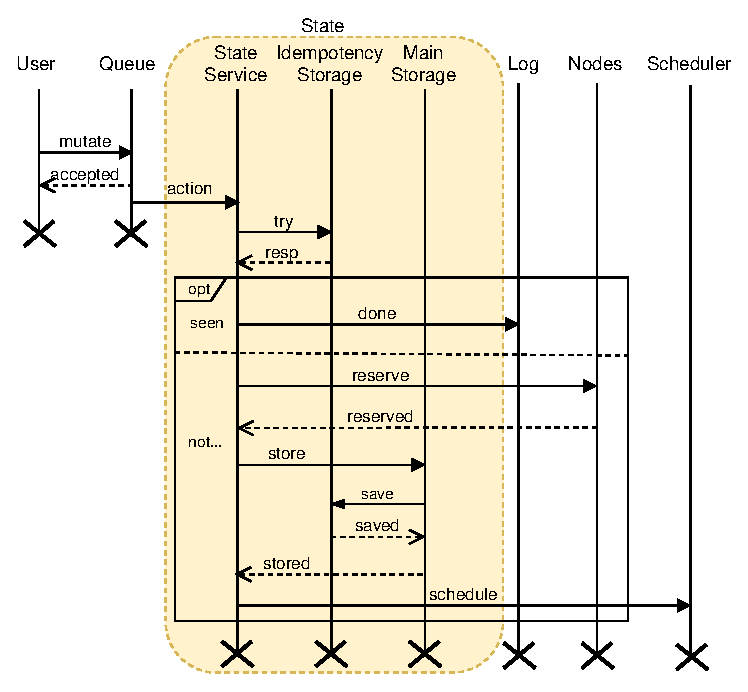
\includegraphics[scale=0.7]{images/Figure13}
	\end{center}
	\vspace{-0.7cm}
	\caption{Low level view of idempotency check communication.}
	\label{fig:fig13}
\end{figure}

The participants follow the communication that we now describe informally:
\begin{enumerate}[start=1,label={(\bfseries \arabic*)}]
	\item \textbf{User} sends a list request to State service (same as~\ref{sec:cluster_formation_protocol});
	\item \textbf{Queue} accepts the list request and the query local state based on the user selector. If a detail view is required, the state gets metrics data from Nodes service (same as~\ref{sec:cluster_formation_protocol});
	\item \textbf{State service} service that is wrapper aroud system main storage. Interacts with main storage in oreder to create new topologies, regions or clusters, or to get data from main storages about same entities.
	\item \textbf{Idempotency storage} contains idempotent set for all \textbf{already} formed topologies, regions and clusters.
	\item \textbf{Main storage} contains records about desired state for all formed topologies, regions and clusters.
	\item \textbf{Log} contains records of operations. Users can query this service to see if their tasks are finished or have any problems (same as~\ref{sec:cluster_formation_protocol});
	\item \textbf{Nodes} accept messages from State. If possible, it will reserve desired nodes, otherwise it will send an error message to Log service. On a health-check message, if a node is used in some cluster, it will inform that the node is alive (same as~\ref{sec:cluster_formation_protocol});
	\item \textbf{Scheduler} waits for a message sent from State, and pushes clus- ter formation messages to desired nodes (same as~\ref{sec:cluster_formation_protocol});
\end{enumerate}

Algorithm~\ref{alg:alg6} describe steps requred to test if operation is done before.

\begin{algorithm}[H]
	\SetKwFunction{idempotent}{idempotent}
	\SetKwProg{Fn}{function}{:}{}
	\Fn{\idempotent{$stored$, $topology$}}{
		\ForEach{data $\in$ topology}{
			\If{isNotSet(data)}{
				\uIf{data.intersection(stored) = data}{
					\KwRet{true}
				}
				\KwRet{false}
			}
			\Else{\idempotent{$data, topology$}}
		}
	}
	
	\SetAlgoLined
	\SetKwInOut{Input}{input}
	\Input{request}
	id $\leftarrow$ seenBefore(request.payload.name)\\
	\uIf{id = null}{
		return true;
	}\Else{
		stored $\leftarrow$ storage.findRequest(id)\\
		topology $\leftarrow$ request.payload.topology\\
		\KwRet{\idempotent{$stored, topology$}}
	}
	\caption{Mutate idempotency check}
	\label{alg:alg6}
\end{algorithm}

Next we present a formal description of the idempotency check protocol (cf. Figure~\ref{fig:fig13}) by using~\cite{HuY17}.
%
%
\subsection{List detail protocol}\label{sec:list_detail_protocol}
%
The last communication protocol in our system appears in the information retrieval process. Namely, on formed topologies, using labels, the user can specify what part of the system he wants to retrieve, for example to visualise on some dashboard. Two options are available: 

\begin{enumerate}[start=1,label={(\bfseries \arabic*)}]
	\item \textbf{global view} of the system --- all topologies the user manages
	\item \textbf{specific clusters} details --- complete details about specified clusters like resources utilization over time (using stored metrics information), node information, and running or stopped services.
\end{enumerate}

It is important to note, that similar to the query operation, both rules $(\ref{eq:eq1})$ and $(\ref{eq:eq2})$ must be satisfied in order for information to be present in the response. 

One additional information may be specified is whether the user wants a detailed view or not. If detail view information is presented in a request, the user will get a detailed view. 

Figure \ref{fig:fig8}. shows a low-level view of the list operation protocol, where users can get details about the formed system. In this setting, the system involves participants: User, State, Nodes, and Log. 

\begin{figure}[!htbp]
	\begin{center}
		\includegraphics[scale=0.9]{images/FIG4}
	\end{center}
	\vspace{-1.2cm}
	\caption{Low level view of list operation communication.}
	\label{fig:fig8}
\end{figure}

We now informally describe the participants roles in the protocol:\label{list_protocol_informal_description}

\begin{enumerate}[start=1,label={(\bfseries \arabic*)}]
	\item \textbf{User} sends a list request to State service;
	\item \textbf{State} accepts the list request and the query local state based on the user selector. If a detail view is required, the state gets metrics data from Nodes service;
	\item \textbf{Nodes} contain node metrics data, and if required, it may send this data to State;
	\item \textbf{Log} contains records of all operations. Users can query this service.
\end{enumerate}

Algorithm \ref{alg:alg5} describes steps after the state receives a list message.

\begin{algorithm}[H]
	\SetAlgoLined
	\SetKwInOut{Input}{input}
	\Input{request}
	Initialize: data $\leftarrow$ []\\
	\ForEach{(topology, isDetail) $\in$ userData(request.query)}{
		\uIf{isDetail}{
			data.append(topology.collectData())\\
		}\Else{
			data.append(topology.data())\\
		}
	}
	\Return data
	\caption{List of current state of the system}
	\label{alg:alg5}
\end{algorithm}

Next we present a formal description of the list communication protocol (cf. Figure \ref{fig:fig4}) by using~\cite{HuY17}.
Global type $\G_3$ (given below) starts with $\mathtt{user}$ connecting $\mathtt{state}$ with one of the two possible messages: 
$(1)$ $\mathit{list}$, specifying a request for a detailed view, where sort $\T_1$ identifies which parts of the system user wants to view in details, after which $\mathtt{state}$ connects $\mathtt{nodes}$ with $\mathit{query}$ message, with a payload of sort $\T_2$  containing specification of which nodes need to show their metrics data, and then protocol proceeds as prescribed with $\G'$; 
$(2)$ $\mathit{list^*}$, specifies no need for a detailed view is specified, where a payload of sort $\T_4$ denotes user specified parts of the system the user wants to view, but without greater details. In the latter case protocol follows global type $\G''$.
\begin{align*}
\G_3 &= 
\left\{
\begin{array}{@{}l@{}}  
\mathtt{user} \twoheadrightarrow \mathtt{state}{:}\mathit{list}(\T_1).\mathtt{state}\twoheadrightarrow\mathtt{nodes}{:}\mathit{query}(\T_2). \G' \\
\mathtt{user} \twoheadrightarrow \mathtt{state}{:}\mathit{list^*}(\T_4).\G''
\end{array} \right.
\end{align*}

Global type $\G'$ starts with $\mathtt{nodes}$ replying to $\mathtt{state}$ $\mathit{result}$ message and a payload identifying parts of the system user wants to see in greater detail typed with $\T_3$. Then, $\mathtt{state}$ connects $\mathtt{log}$ with $\mathtt{details}$ and also sends $\mathtt{result}$ to $\mathtt{user}$, and finally terminates. 
In $\G''$, $\mathtt{state}$ also connects $\mathtt{log}$ with $\mathit{brief}$ and a payload typed with $\T_5$ identifying parts of the system user wants to see without greater detail. Then, $\mathtt{state}$ replies to $\mathtt{user}$ with $\mathtt{result}$ message, and the protocol terminates.
\begin{align*}
\G' =  & 
\mathtt{nodes}\to\mathtt{state}{:}\mathit{result}(\T_3).\mathtt{state}\twoheadrightarrow \mathtt{log}{:}\mathit{detail}(\T_3). \\
& \hspace{2mm}
\mathtt{state}\to\mathtt{user}{:}\mathit{result}(\T_3).\tend\\
\G'' = &
\mathtt{state}\twoheadrightarrow \mathtt{log}{:}\mathit{brief}(\T_5).\mathtt{state}\to\mathtt{user}{:}\mathit{result}(\T_5).\tend
\end{align*}

Same as for the health-check and the cluster formation protocols, here we also present the projections of global type $\G_3$, modeling the list protocol, onto participants $\mathtt{user}$, $\mathtt{state}$, $\mathtt{nodes}$, and $\mathtt{log}$:
\begin{align*}
\ST_\mathtt{user} =& 
{+}
\left\{
\begin{array}{@{}l@{}}  
\mathtt{state}{!!}\mathit{list}(\T_1).\mathtt{state}{?}\mathit{result}(\T_3).\tend \\
\mathtt{state}{!!}\mathit{list^*}(\T_4).\mathtt{state}{?}\mathit{result}(\T_5).\tend 
\end{array} \right. \\
%
%
\ST_\mathtt{state} =&
{+}
\left\{
\begin{array}{@{}l@{}}  
\mathtt{user}{??}\mathit{list}(\T_1).\mathtt{nodes}{!!}\mathit{query}(\T_2).\ST'\\
\mathtt{user}{??}\mathit{list^*}(\T_4).\mathtt{log}{!!}\mathit{brief}(\T_5).\mathtt{user}{!}\mathit{result}(\T_5).\tend
\end{array} \right. 
\end{align*}
where
\begin{align*}
%
\ST'  =& 
\mathtt{nodes}{?}\mathit{result}(\T_3).\mathtt{log}{!!}\mathit{detail}(\T_3).\mathtt{user}{!}\mathit{result}(\T_3).\tend\\
%
%
\ST_\mathtt{nodes} = &
\mathtt{state}{??}\mathit{query}(\T_2).\mathtt{state}{!}\mathit{result}(\T_3).\tend \\
%
%
\ST_\mathtt{log} = & 
{+}
\left\{
\begin{array}{@{}l@{}}  
\mathtt{state}{??}\mathit{detail}(\T_3).\tend \\
\mathtt{state}{??}\mathit{brief}(\T_5).\tend \\
\end{array} \right.
\end{align*}

For instance, type $\ST_\mathtt{log}$ specifies $\mathtt{log}$ gets included in the session only after receiving from $\mathtt{state}$, either message $\mathit{detail}$, or message $\mathit{brief}$, and then terminates. 

Similarly as for $\G_2$, we remark $\G_3$ could also be modeled using standard MPST (e.g.,~\cite{HondaYC08}), but again the projection types would be undefined, while following the approach of ~\cite{HuY17} with explicit connections, we have obtained all valid projections.
%
%
\section{Repercussion}\label{sec:repercussion}
%
Model presented in this chapter, have two possible repercussions:

\begin{enumerate}[start=1,label={(\bfseries \arabic*)}]
	\item \textbf{Stand alone}, the proposed model can serve as a base layer for future ECC as a service implementation. On top of it, we can implement other services and features like scheduling, storage, applications, management, monitoring, etc. As such it could be valiable option in the CC.
	\item \textbf{Integration}, the proposed model could be integrated with existing systems like Kubernetes, OpenShift, or cloud provider infrastructure since they all operate over the cluster. This is possible, with some small infrastructure changes and adaptations because --- the communication should implemented via standard interfaces like HTTP and JSON, the integrations should be relatively easy to achieve. The proposed model could be used as a geo-distributed description and/or an  organization tool.
\end{enumerate} 
%
%
\section{Limitations}\label{sec:limitations}
%
Since the perfect model never existed, model that is proposed in this thesis have some limitations, that we must be aware of. Either to work on improvements, or use the model as is. When talking about small scale servers and micro-clouds, we must be aware of the few things. 

\begin{enumerate}[start=1,label={(\bfseries \arabic*)}]
	\item not all companies and organizations will be able to deploy them, due to the high investments required~\cite{MonsalveCC18}. Similar to the cloud where massive DCs are built by a few companies and used by many others. These small servers could be deployed by government authorities or large cloud companies for their own needs. The general public can use them, similarly to the cloud --- pay as you go, model.
	\item there is no guarantiee that existing public cloud providers will allow nodes that are not built, resigned or deployed by them. If we are building private cloud, thant we can make different decision. One way to resolve this issue is that whole platform become open-source, so that public cloud providers can engage into development, and eventually use tham as a solution.
	\item These small scale servers must be out of reach of people, and protected in some way so that not everyone have access to them. Some degree of phisical security mut be implemented.
	\item places where these small scale servers will be deployd must have stable internet connection, and ability to integrate SDN or other similar techologies, so that complex network topologies could be implemented properly.
	\item these servers can have some open architecture or could be custom built by other providers. In both cases they must be able to satisfy rules that are presented in~\ref{sec:separation_of_concerns}.
\end{enumerate}
%
%
%!TEX root =  main.tex
\chapter{Proof of concept}\label{chapter:Implementation}
%
In this chapter, more details are going to be given about the framework implemented based on the formal model and architecture specification given in the previous chapter.

Section~\ref{sec:framework} discusses framework architecture, and system implementation details, and framework limits. Section~\ref{sec:framework_operations} presents implementation details about framework operations. Section~\ref{sec:app} describes few possible senarios and applications that could utilize micro-clouds platform. In Section~\ref{sec:results} presents results of our experiments.
%
%
\section{Platform implementation}\label{sec:framework}
%
In this section, we are going to introduce an implemented proof-of-concept framework based on the model proposed in the previous chapter~\ref{chapter:Micro_clouds}. The framework is called \textbf{Constellations} or \textbf{c12s}\footnote{https://github.com/c12s} for short because it is strongly influenced by nature and the neverending number of galaxies that the universe is (not only) composed of. Similarly, we are trying to create a universe of clusters that will serve humanity to help them with their day-to-day tasks. The framework is \textbf{open-source}, and it is implemented using the microservice architecture with services that have distinct role and purpose to the entire system. These services are:

\begin{itemize}
	\item \textbf{Gateway}, this purpose is to export services feature to the rest of the world. Gateway is designed as a REST service, accepting $JSON$ style messages, so that various clients can communicate to the system. When the request arrives at the gateway, if the request is valid it will pass the request to the rest of the system. It communicates to the rest of the services to check if the user exists, if he / she has proper rights for actions he / she sends, and if not, returns the proper message and and does not propagate it to the rest of the system.
	\item \textbf{Authentification \& Authorization}, the sole purpose of this service is to store users and their credentials. This service will validate does user exists in the system, and does he have certain rights to perform some specific operation. Users that often use the system will be stored in the cache layer of the service so that on the next request his actions are done faster. Users that do not use the system that often will not be stored in the cache, until the first use. After that, if the user does not use the system for some time, he/she will expire from the cache.
	\item \textbf{Queues}, the purpose of this service is to prevent huge request load to the system and to accept more user requests. When the user submits any \textbf{mutation} operation -- an operation that changes the state of the system, these operations will be put in the queue. User can create their queues, to prevent long lines for specific tasks. For example, users can create queues for specific tasks, and use them only for those tasks, while other queues could be general-purpose queues. On system start, every user will start with one queue --- \textbf{default}. When doing mutations on different parts of the system, the user can specify in metadata which queue he wants the task to go to. This service implements a token bucket rate-limiting algorithm~\cite{MathewsKG17} to prevent congestion of the system.
	\item \textbf{Nodes}, this service stores and maintains pieces of information about registered nodes in the system. All node hardware and software details will be stored in this here. This service is also responsible for storing metrics data, accept health-check requests from nodes, and inform the rest of the system that the used node is alive.
	\item \textbf{State}, is the heart of the system. This service stores all information about architecture, clusters, regions, and topologies. When a new cluster/region/topology is created, this service will setup watchers for nodes, so that if the node does not send the health-check signal for some time, that node will be declared dead. This is important so that at any moment we must know the state of the clusters and their utilization. This service as well will cache frequently used nodes data, so that on the next request node lookup is faster, since we can have a huge number of nodes, topologies, clusters and pieces of information about them. To prevent data loss, this service will first store a copy of the operation before attempting any mutation of the system.
	\item \textbf{Log}, is responsible for storing all log and trace data from every service. Here a user can check whether all jobs are done, whether there is some error and possibly why the error happened to resolve it or fix it for the next time. From a user point of view, this is \textbf{read only} service and from a system view, this is \textbf{write only} service.
	\item \textbf{Command push}, the purpose of this service is to push commands and operations to the nodes user desired. This service implements a token bucket rate-limiting algorithm~\cite{MathewsKG17} to prevent constant data push to the nodes. Similar to the state service, this service will store a copy of operation information locally before attempting any push to the nodes. This information will be deleted, once the operation reaches all decided nodes and all of the responses with the acknowledge (ACK) message.
\end{itemize}

\noindent
All services are highly customizable and all have their configuration file that could be changed and adopted. All these services are easy to extend to support new operations and pieces of information about nodes, regions, clusters, topologies, and latter on applications, configurations, namespaces, etc. 

The system operates with four commands, where three of them follow formal models described in the previous chapter. The last command is a simple command to list logs for every user.

Regarding~\ref{sec:access_pattern}, the framework operates as a master process is running in Kubernetes, and through that process, all commands are issued. Future applications can communicate with nodes as stated in~\ref{sec:application_model}. They do not require communication with the master process at all, they can communicate with the formed cluster using topics and streams.

In the rest of this section, we will see details about all operations, as well as used technologies to implement the whole system. Possible applications and future directions for application development will also be described. System architecture is shown in Figure~\ref{fig:fig11}.

\begin{figure}[H]
	\begin{center}
		\includegraphics[scale=0.7]{images/FIG5}
	\end{center}
	\vspace{-0.5cm}
	\caption{Proof of concept implemented system.}
	\label{fig:fig11}
\end{figure}
%
%
\subsection{Technologies}\label{sec:technologies}
%
All services are implemented using the Go\footnote{https://golang.org/} programming language, because of its well-known tooling, support for developing system software, web-based applications, small binaries but also, great concurrency model, and ability to build binaries for almost any architecture without any code changes. All services rely on Go implicit \emph{interface} implementation mechanism. Every technology or component used in the system can be swapped for some other, as long as that component implements \emph{interface} fully. The framework is developed in such a way that is relatively easy to extend, or switch and use different components and technologies.

As the main storage layer for our system, we used etcd\footnote{https://etcd.io/}, a popular open-source key-value database, that shows good performance, and it is mostly used for configuration data. Metrics data are stored in the open-source time-series database InfluxDB\footnote{https://www.influxdata.com/}. 

Communication between microservices is implemented in RPC manner using gRPC\footnote{https://grpc.io/}, and Protobuf\footnote{https://developers.google.com/protocol-buffers} as a message definition. gRPC and Protobuf are open-source tools designed by Google to be scalable, interoperable, and available for general purposes. Communication between nodes and the system is carried out using NATS, an open-source messaging system. Health checking and action push to nodes are implemented over NATS\footnote{https://nats.io/} in a publish-subscribe manner.

Caching layer for every service is implemented using Redis\footnote{https://redis.io/} key-value, in-memory database. It is important to notice, that all concrete tools that are used, are easily swappable for some other as long as they implement a proper interface.

All communication with the outside world is done in a REST manner using JSON encoded messages over HTTP. To communicate with the platform, we have developed a simple command-line interface (CLI) application also using the Go programming language that sends JSON encoded messages over HTTP to the system.

Every service is packed in a container, and for this purpose Docker\footnote{https://www.docker.com/} containers are used. To achieve automatic orchestration, and self-heal, and up-time, all services that are packed in containers, are running inside Kubernetes.

Every service will log details about its usage and calls, as well as traces how requests are going. Log data is stored outside the service and container, and pieces of information will be sent to centralized log storage on every $t$ seconds specified by the user. Sending intervals could be changed and adapted using the configuration file for every service independently.

Log data will be stored in the two levels:

\begin{enumerate}[start=1,label={(\bfseries \arabic*)}]
	\item \textbf{system level}, this data is generated by the system and could be viewed by administrators of the system \textbf{only}. Operations people in the team (eg. DevOps or SREs), and developers cannot see it, but providers can.
	\item \textbf{user level} that stores information about user requests that \textbf{only} users can see. This type of data will not be visible to the developers of the system, and only users that created these logs will be able to see them.
\end{enumerate}

\noindent
Log storage could be searched to see the general state of the system, and pieces of information about user requests and the state of their requests.
%
%
\subsection{Node daemon}\label{sec:node_daemon}
%
Every node runs a simple daemon program implemented using the Go programming language, as an actor system (Ref. secion~\ref{sec:actor_model}). The actor system is developed for this purpose. When a message arrives, the proper actor will react based on the message type, or discard it if the type is not supported. 

Extending such a system is rather easy because users need to simply write a new actor and logic that goes with them and register it to the system.

When the daemon start, it will first read the configuration file to do the proper setup and then will contact the actor system to start all the actors. 

System messages will be sent to the daemon, but it will not react to these messages. Daemon is not able to communicate with any actor directly. All communication goes through the actor system which is responsible to pass messages to the actors. The actor system at this point has only four existing actors:

\begin{enumerate}[start=1,label={(\bfseries \arabic*)}]
	\item \textbf{cluster actor}, this actor reacts on messages about new cluster formation, but he is also responsabile to contact rest of the system that message has arrived.
	\item \textbf{internal actor}, this actor react to messages from other actors to update the daemon state. For example, on new cluster creation, this actor will update daemon id, name, labels, etc.
	\item \textbf{health actor}, this actor will periodically send \emph{health-check} data to the system about node state, utilization, etc. This actor will communicate to the rest of the hardware to get proper pieces of information, to collect logs from the node, and send all that data to the system.
	\item \textbf{gossip actor}, this actor will communicate with other peers in the group using SWIM protocol techniques.
\end{enumerate}

\noindent
The actor system will monitor these actors, and in case any of the crushes, the actor system will restart them. 

Listing~\ref{lst:listing3} show the actor system hierarchy of existing actors.

\lstinputlisting[caption={Actor system hierarchy.}, label={lst:listing3}, captionpos=b, xleftmargin=.35\textwidth]{listings/listing3.txt}

\noindent
Before daemon starts, the user needs to specify some parameters for proper configuration like: 

\begin{enumerate}[start=1,label={(\bfseries \arabic*)}] \label{imp:features}
	\item \textbf{identifier}, represents unique identifier of the node. When a node is not a part of some cluster, this can be whatever the user wants. Once the node is a part of some cluster, the identifier will be updated, and it is not advised to change it manually afterwards.
	\item \textbf{name}, represent name of the node. This property also can be changed when a node is part of the cluster, otherwise, it can be whatever we want.
	\item \textbf{labels} represent the specific features of the node. Labels are used to query for free nodes, and there is no formal restriction of what they can or can not be. This property can be changed when the node is a part of some cluster. It is advised that as labels we put some specific features of the node that might be beneficial for the user who is looking for nodes to create new cluster/s.
	\item \textbf{health-check details}, here we have pieces of information to control the health-check mechanism. Since nodes communicate with the rest of the system via publish-subscribe events, we must specify the address of the rest of the system and the topic name, where we publish our pieces of information.
	\item \textbf{system information}, represents basic information for a node to know how to contact the rest of the system. We should specify the system address, so that node knows where to send messages, and where are messages are coming from. We can also specify the version of the system we are trying to contact. System version could be used to support \textbf{backward compatibility} if we have multiple API versions of the system running at the same time or some period.
\end{enumerate} 

\noindent
Configuration can be done easily using the YAML configuration file. 

Listing~\ref{lst:listing1} shows simple YAML configuration file for daemon process.

\lstinputlisting[caption={Daemon configiration file}, label={lst:listing1}, captionpos=b, xleftmargin=.35\textwidth]{listings/listing1.yaml}

\noindent
Based on the configuration file, the daemon will start a background health-check mechanism, and it will subscribe to the system, using an identifier as a subscription topic. The background thread will contact the system repeatedly using a contact interval time, specified in the configuration file. 

On every health-check, the node will send labels, names, IDs, and metrics to the system (e.g., CPU utilization, total, used, free ram or disk, etc.). The specified labels will be used when the user is querying for available nodes, while the node id will be used for reservation when forming a cluster.

At the first start of the daemon, when the node is free, the user can specify whatever node id he/she wants. Once, the node is a part of the cluster, the node id will be updated to match that. Node id update will happen on the cluster formation process.
%
%
\subsection{Separation of concerns}\label{sec:framework_SoC}
%
IThe implemented framework follow the clear SoC model, presented in~\ref{sec:separation_of_concerns}. Since the presented model consists of three components, the implemented framework is deals only with \textbf{resources}~\ref{soc:resources} part of the SoC. 

Its job is to organize nodes into clusters, regions, and topologies, to make them communicate and expose their resources to the upper layer of SoC for utilization. The upper layer will run services on these resources, to collect data from data creators and process them as requested.

The upper layer must have set up the infrastructure to do any processing or storage. This middle layer is the binding element between the layers.
%
%
\subsection{Long-lived transactions}\label{sec:transaction}
%
Current implementation follows the sagas pattern (cf.~page~\pageref{sec:sagas}) for transactions, and isolation is added using semantic lock by adding states to the task. The task can be in one of following states: \textbf{(1)} \emph{PENDING}, \textbf{(2)} \emph{IN PROGRESS}, \textbf{(3)} \emph{CREATED}, and \textbf{(4)} \emph{FAILED}. 

Until the task reaches \emph{Created} state, no other operation can be done on that cluster configuration.

The cluster formation transaction is split into a few sub-transactions: \textbf{(1)} reserving nodes, \textbf{(2)} writing cluster information, and \textbf{(3)} sending cluster information to push service and ultimately sending pieces of information to the nodes. 

The rollback mechanism is implemented using \emph{choreography}, and communication between the various services is done asynchronously using message queues.
%
%
\subsection{Garbage collection}\label{sec:gc}
%
The current garbage collection process is pretty trivial since there is no complicated graph of items connected to the cluster information details.

The process will scan tasks with the state \emph{FAILED} in the background, and it will remove those items. Related details to the cluster information, for example, node metrics, will expire automatically since there is a lease attached to them.

Another resource that will be automatically deleted is node data. If a node health-check message does not reach the system in some time, the node lease will expire and data will be removed automatically.
%
%
\subsection{Limitations}\label{sec:framework_limits}
% 
The framework at the current state has some limitations that we \textbf{must address}. As shown in figure~\ref{fig:fig11}, for purpose of testing the system, and to give the users any way to interact with the system, a CLI application is implemented. This is a good option for initiating commands to the system. The problem with this approach is that showing logs, and topologies might be limiting the users, especially if they monitor and supervise multiple topologies with regions and clusters.

For monitoring, a tool with UI would be a better solution and it can show more details. For a small amount of data, when topologies are relatively small, CLI could be used. But for some real-world applications, desktop, and/or web-based UI will be a much better solution, and CLI can be used for fast lookup on specific pieces of information about clusters and nodes, for example.

The current implementation of the queueing system is \textbf{limiting} because if we want to extend the system with new queues we need to shut down the whole service, and that is not the best solution. But since the goal of this thesis is not queue management, but micro-cloud formation, protocols, and formal modeling.

Since the goal of this thesis is not queue management, and the purpose of this thesis is not Human-computer interaction, but micro-cloud formation, protocols, and formal modeling, mentioned limitations should be the topic of the future work~\ref{sec:future_work} section.

The current implementation do not include garbage collection of connected dependent items, and users cannot influence garbage collection decisions. This should be one of the topic of the future work~\ref{sec:future_work} section as well.
%
%
\section{Operations}\label{sec:framework_operations}
%
In this section, we are going to describe all implemented operations in the framework and present specific details about every individual operation.
%
%
\subsection{Query}\label{sec:query} 
% 
The query operation is used to show all free nodes or filtered free nodes that are registered into the system, to the user (yellow arrows in Figure~\ref{fig:fig11}.). 

When a user wants to get information about free nodes, they need to submit a \textbf{selector} value which is composed of multiple \textbf{key-value} pairs.  These key-value pairs can be any alphanumeric set of symbols for both keys and values. Based on that key-value pair the system will do the query of the free nodes.

The selector will be used as a search mechanism to compare the labels of every free node that exists in the system. The nodes that are satisfying the rules~\ref{frm:query_rule} defined in Section~\ref{sec:cluster_formation_protocol} will be present in the result.

This operation is done before the formation of new topologies, regions, or clusters --- mutation of the system. The user first needs to get a list of free nodes, then he can choose nodes that are best suited for him and try to form topologies, regions, or clusters of them.

The querying process is a little bit changed from one presented in Section~\ref{sec:cluster_formation_protocol}. The only change that is made is the addition of the \emph{Gateway} service that will pass requests into the system and prevent overflow of requests. This change \textbf{does not} affect or validate the formal model presented before, since the added service does not interfere with the process of searching nodes or changes to the system.

Figure~\ref{fig:fig14} shows a communication diagram for the query action, with the addition of the Gateway service.

\begin{figure}[H]
	\begin{center}
		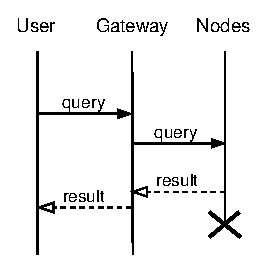
\includegraphics[scale=1]{images/Figure14}
	\end{center}
	\vspace{-0.7cm}
	\caption{Low level communication protocol diagram of query operation.}
	\label{fig:fig14}
\end{figure}

\noindent
Query operation is implemented using \emph{api composition} pattern (cf.~page~\pageref{par:composition}).
%
%
\subsection{Mutate}\label{sec:mutate} 
%
Mutate operation (orange arrows in Figure~\ref{fig:fig11}.) changes the system state by creating, editing, or deleting clusters, regions, and topologies. When a user wants to perform a mutation over the system, the desired state needs to be specified \textbf{declaratively} using a YAML file and submitted to the system. When the state is submitted, the system will do the rest of the job to ensure that the state desired by the user is reached.

The users specify which nodes are forming the cluster. Optionally, users can also specify labels and names on the node level, and retention period on the cluster level. The retention period is used to describe how long metrics are going to be kept. When the retention period expires, the metrics data will be deleted or moved to another location. 

When forming a topology, users can assign a name and label to the entire topology. These parameters will be used when the user wants to query all topologies to get full information about regions, clusters, and nodes inside a topology.

Mutate operation is \textbf{immutable}, which mean that there will be no in-place changes to the existing state. If a user wants to do any update, he/she needs to specify a full new state that will replace the existing one. This operation is \textbf{atomic} as well, which mean that a whole new state must be able to replace the existing state. If this happens, the system will replace the old state with the new one. The main storage that stores configuration data is a key-value store implemented using an etcd database. The key that will be used to store the configuration data is the whole path of topology, regions, cluster, node, while the value represents the state desired by the user. 

Listing~\ref{lst:listing4} shows structure for key-value pair that is stored in the main database, where on top we can see a structure of the \textbf{key}, and below it we can see the structure of the \textbf{value}. This kind of structure is similar to OS file-system data organizations of files and folders.

\lstinputlisting[caption={Structure of stored key-value element.}, label={lst:listing4}, captionpos=b, xleftmargin=.25\textwidth]{listings/listing4.txt}

\noindent
We store as well one additional information about labels \textbf{index} value. This index is used for a faster query of elements when doing labels comparison. To find elements we can query in a similar way like searching files and folder structure. The etcd in newer version \textbf{do not allow} hierarchical keyspace, but what they allow is \textbf{ranged} query by some \textbf{prefix}. This is useful as well because we can still get all regions in topology, clusters in the region, or nodes in the cluster if we know to which group they belong.

Mutate operation is not idempotent by nature, but the whole process behind it makes mutate an idempotent operation. Whether the user tries to create already existing infrastructure by changing the order of regions, clusters, or labels in the nodes, or if he for whatever reason did not get confirmation that infrastructure is created, an existing infrastructure will not be created. This is done in such a way, that $State$ service (Figure~\ref{fig:fig11}) will keep the information set about created infrastructure. This information is implemented as a \textbf{flat keyspace} set, that have information. On every mutation request, the system will test if such a topology already exists. If such topology already exists, the user will get confirmation that his infrastructure is created. If such topology do not exist, a new cluster formation protocol~\ref{sec:cluster_formation_protocol} will be initiated. The mutation confirmation is followed by a \textbf{unique id}, which the user can use to query steps, logs, and traces that are done in process of working towards the state desired by the user. Logs service can give the user complete details about his task state using that unique id.

When creating topologies, the user is free to give whatever name he wants for every region, cluster, and node. The only restriction is that name should be the alphanumeric set of characters. Listing~\ref{lst:listing2} shows an example of a user-defined state that forms the topology of one region with one cluster that contains three nodes, with a retention period of 24 hours. The whole topology will have the same set of labels, but $node3$ redefines this rule by specifying its own.

\lstinputlisting[caption=Example of mutate file using YAML., label={lst:listing2}, captionpos=b, xleftmargin=.3\textwidth]{listings/listing2.yaml}

\noindent
After all, nodes that should form a cluster, acknowledge cluster formation message, they will inform the system that the message is received, and they will start the process of cluster formation. This process is done by using SWIM~\cite{DasGM02}, a Gossip style protocol. When every node has a complete list of its peers that should be in the cluster, the process of cluster formation is done. 

On the next health-check message, every node will send its \textbf{id} that is telling the system that he is part of some cluster. This kind of messages will be used in the $State$ service to validate that cluster is alive and well, or that some nodes (or all), are dead or down if \textbf{id} is not received. 

Gossip style protocols (like SWIM) could be used in the future to propagate information in the cluster, without explicitly ping every node in the cluster.
%
%
\subsection{Queueing}\label{sec:queueing}
%
When doing mutation, users can target a specific system queue, by adding a metadata part in the configuration file. With this ability, users can aim for specific queues just for the mutation to avoid long waiting times if other queues are full. Currently, the system does not have any limitations, restrictions, or logic that will specify which queues are used for what or give them special rules or permissions. This can be viewed as a \say{gentleman agreement}, that in one team, operations users can proclaim specific queues like \textit{mutatation} queues used maybe for specific topologies, and later on for other operations as well.

The queue service starts only when the $default$ queue exists. Adding a new queue to the system is implemented using the configuration file, for convenience only. 

Listing~\ref{lst:listing5} shows an example of queue service with two additional queues with specifications of their parameter needed for token bucket operation~\cite{MathewsKG17}. Also, we can see configuration pieces of information for instrumentation of a single service, and the same configuration is implemented for all specified services shown in Figure~\ref{fig:fig11}.

\lstinputlisting[caption={Structure of stored key-value element.}, label={lst:listing5}, captionpos=b, xleftmargin=.25\textwidth]{listings/listing5.txt}
%
%
\subsection{List}\label{sec:list} 
% 
The list command shows the current state of the system for the logged user (blue arrows in Figure~\ref{fig:fig11}.). Logged user is able \textbf{only} to see infrastructure he/she has created or maintains. All other infrastructures, created by other users, will not be visible to the users that are not creators or maintainers.

To view his/her infrastructures, the user can specify what part of the system he/she wants to see using a set of labels or list of key-value pairs, which will be used by the system to determine what the user wants to see. This process is similar to \textbf{selector} shown in the query~\ref{sec:query} operation. 

There are two levels of details that user can specify:

\begin{enumerate}[start=1,label={(\bfseries \arabic*)}]
	\item \textbf{global view}  of the syste, or all topologies he/she manages with just basic information like resource utilization, number of regions clusters and nodes.
	\item \textbf{detail view}, or details about a single topology (i.e., regions, clusters, and nodes in a single topology). Users can specify a more detailed view of a single cluster, meaning the users will get information about what resources the cluster has, but also resource utilization over time (using stored metrics information) and so on.
\end{enumerate}

\noindent
Both options can be useful if operations people need different details levels for different topologies. List operation is implemented using \emph{api composition} pattern (cf.~page~\pageref{par:composition}).
%
%
\subsection{Logs}\label{sec:logs}
% 
The logs operation shows stored logs and traces to the user (purple arrows in Figure~\ref{fig:fig11}.). Same as previous operations, the user needs to be registered and logged in to be able to perform this action. With this action, the user can see the state of his/her operations and actions. The user can choose between two options for querying his/her logs:

\begin{enumerate}[start=1,label={(\bfseries \arabic*)}]
	\item \textbf{get}, for this option a user needs to provide a unique task id that is given to the user when he/she creates a mutate operation. With this option, the user will get a full list of steps, traces, and logs collected over the time the system was setting up his/her desired state.  
	\item \textbf{list}, with this option user can specify \textbf{selector} using list of key-value pairs in a similar way to query~\ref{sec:query} and mutate~\ref{sec:mutate} to filter only parts of the traces that contain the same labels as selector does.
\end{enumerate}

\noindent
This action is implemented in some basic aspects, as this action can return a huge amount of data that require some better visualization than CLI.
%
%
\section{Results}\label{sec:results}
% 
For the ease of testing, a few ARM-based nodes that are easy to move from place to place have been used. The test should be conducted on the heterogeneous nodes, to see how the system will react to different architectures and resources. In our tests, we have used:

\begin{itemize}
	\item 9 Raspberry Pi 3+ Model B with 1GB LPDDR2 SDRAM, 16GB SDCard storage, and 1.4GHz Cortex-A53 64-bit SoC running Raspbian Linux, a Debian-based operating system.
	\item 3 Beagle bone black devices with 512MB DDR3 RAM, 4GB 8-bit eMMC on-board flash storage, and 1GHz ARM Cortex-A8 running a version of Linux Debian operating system.
\end{itemize}

\noindent
as test heterogeneous nodes for creating clusters, regions, and topologies.
%
%
\subsection{Experiment}\label{sec:experiment}
%
Using Go tooling, we were able to build daemon service without changes and dissiminate on all nodes without problems.

We ran tests on different configurations and different nodes clusters using these nodes. All nodes were connected on the network, and experiments were conducted in a controlled environment. Nodes that should be a part of the same cluster were connected on same network for easier experiments.

Experimental research was realized in the laboratory of the Department of Informatics at the Faculty of Technical Sciences in Novi Sad. The laboratory of the Department of Informatics is equipped with adequate computer, communication and software equipment on which the set goals in this thesis can be fully realized.

Our experiment started with separating nodes into groups of \textbf{three}. This number is chosen because in DS, an odd number is used in cases when we need to reach some agreement and we need major majority like consensus, for example. This is not important for purpose of this thesis, we could pick any number, membership protocol does not makes a difference if there are three or four or eleven nodes in the cluster.

After nodes had been separated, we created a configuration file for every node, setting up default parameters for every property node daemon required~\ref{imp:features}. After all services were up and running, we turned the nodes on, and health-check protocol~\ref{sec:health_check_protocol} started at uprfront defined time, which we had set for test purposes at \emph{1 minute} interval. Logs, resources and other node details were set to \emph{15 seconds} interval, so between health-check intervals, daemon would collect resource information \emph{four times} before sending it to the rest of the system.

For convenient testing, all nodes had the same set of labels, and as labels we chose OS name, OS version, architecture version, node name basic details about resources of the nodes.

After some time, we were able to see all nodes registered in the system. When all nodes had been sending health-check ping for some time, and we had a stable system, we issued a mutate operation creating clusters of nodes that are logicaly close ot each other, and we initiated cluster formation protocol~\ref{sec:cluster_formation_protocol}. After the protocol was done, we ended up with four clusters as we intended. We tried to initiate the same command again to test idempotency check~\ref{sec:idempotency_protocol}, and we got the message that clusters already existed.

To increase capaticity, we extended clusters by creating new ones using \emph{three clusters} with \emph{four nodes}. We created new new mutate file, and initiate new mutate command. After some time, we saw that one cluster was down and that we now had \emph{three clusters} with \emph{four-nodes}, as we intended. After successful creation of new clusters, we dleted down cluster.

The last test was to test health-check protocol once again - we disconnected one random node from the power supply, and since that node ping was missing, the system was able to detect which node was \emph{down}. This concluded our experiment.
%
\section{The existing solutions enhancement}~\label{enhancement_of_the_existing_solutions}
%
The protocols defined in this thesis could serve as a base layer for the system developed from scratch. On top of such a solution, other services and features can be added like scheduling, storage, applications, management, monitoring, etc. The protocols described in this thesis ensure proper node registration into the system, organization, and reorganization of node resources into clusters, regions, and topologies, bringing disposable micro clouds closer to the users at the network edge, allowing that requests are served from the local micro cloud.

The existing orchestrator engines (e.g., Kubernetes, Apache Mesos, Docker Swarm, etc.) operate one cluster level~\cite{BurnsGOBW16, VermaPKOTW15, RossiCPN20, KubeEdge, KubeMulti}. The single cluster could span over multiple availability zones in the cloud, minimizing the chance that a failure in one zone impairs services in other zones~\cite{KubeMulti}. Kubernetes allow extension in terms of multi-cluster deployments~{\cite{KubeMulti}}. In such a scenario, Kubernetes is handling these clusters as disposable --- "treating \textbf{clusters} as cattle, not pets" (i.e., numerous servers/clusters built using automated tools designed for failure, where no servers/clusters are irreplaceable~\cite{CERN}).

The model proposed in this thesis goes one step further, allowing the creation of disposable micro clouds. Such an extension allows infrastructure optimization in more dimensions~\cite{ForestieroMMPS14}. The users are allowed to build numerous micro clouds designed for failure using automated tools where no micro cloud is irreplaceable --- "treating \textbf{micro clouds} as cattle, not pets."

The existing solutions can integrate the model proposed in this thesis to serve as a node register. Such integration allows the registration of new nodes into the system, allowing the existing orchestration engines to use new nodes, and expand their available resource pool. In form of specification, the users can provide a list of which available EC nodes need to be part of some micro cloud. The system will communicate with the existing orchestrator agent to register/unregister them with the existing cluster. In such a scenario, we can hook on the existing orchestrator health-check mechanism informing our system that a node in some cluster is alive. Unused nodes still use the health-check protocol defined in this thesis informing the system that they are still available for utilization.

The proposed model preserves the node's topology allowing cloud providers and orchestrator engines to treat micro clouds disposable, abstracting infrastructure to the level of software --- infrastructure as software~{\cite{Fitzgerald}}. This approach benefits from the already available tools, principles, and techniques (e.g., reuse, testing, modeling, and evaluation). The already available tools can be used for the disposable micro cloud infrastructure definitions.

The model developed in this thesis is not competing with the existing orchestrator tools. It is not orchestrating applications, but it is a free nodes register and micro clouds infrastructure descriptor allowed to be offered as a stand-alone service bringing disposable micro clouds model to the users. The model allows integration with the existing orchestration tools, leveraging existing mechanisms and best practices. Cloud providers can create an operator for various orchestration engines. This allows them to offer dynamically created, disposable micro clouds as a service to their users, using infrastructure as software principles.
%
%
%!TEX root =  main.tex
\chapter{Conclusion}\label{sec:Conclusion}
%
%


\section{Future work}\label{sec:future_work}
%
%
%
%
\bibliographystyle{elsarticle-num}
\bibliography{bib}\cleardoublepage
%
%
\pagestyle{empty}
%!TEX root =  main.tex
\chapter*{Biography}
\pagenumbering{gobble}
%\pagestyle{empty}

The work in this thesis is synthesis of few individual parts:

\begin{enumerate}[start=1,label={(\bfseries \arabic*)}]
	\item The experience acquired on a university, on the topic of software engineering,
	\item The research conducted as part of the PhD studies, covering various aspects of the distributed systems,
	\item The work done in collaboration with prominent software vendors,
	\item The collaboration with researchers from different research areas.
\end{enumerate}

\noindent
Milo\v s Simi\'c is a Ph.D. student and teaching assistant within the Department of Computing and Control, Faculty of Technical Sciences, University of Novi Sad since 2015. He received his B.Sc. degree in 2014, and M.Sc. degree in 2015, all in Computer Science from the University of Novi Sad, Faculty of Technical Sciences. He is owner of two team awards: $(1)$ Best paper award (academia), and $(2)$ ThinkX in the category Community and Social Impact (industry).\\\\ 
\noindent
Over the years, Milo\v s worked with various prominent software vendors, in different fields. This allowed him combining the different skillsets developed over the years, to focuse his expertise towards designing and implemennting distributed and software systems, for various usages. His research interests include: $(1)$ distributed systems, $(2)$ (multi) cloud computing, $(3)$ edge computing, $(4)$ big data and $(5)$ service oriented architectures and microservices.\\\\
\noindent
As part his Ph.D., Milo\v s have studied the different distributed systems techniques, combined with various software engineering methodologies and practices, covering both standard-defined processes and industry-proven methods, to resolve and answer such complicated questions that are part of this thesis. Working with different softvare vendors, combined with traditional academic research, helped Milo\v s to clear his PhD vision, and guid him to the work that is described in this thesis.\\\\
\noindent
Trough colaboration with people from different research areas, this theis gain forml description and formal model that is important leverage, to describe and validate such complicated system that is described in this thesis.\cleardoublepage
%
%
\end{document}